\section{Additional Experimental Results} \label{app:add_exp}

\subsection{Contrast with LSTMs} \label{app:lstm}

While our primary goal is to analyze Transformers, we also consider LSTMs \citep{hochreiter1997lstm} to understand whether Transformers learn different algorithms than other neural sequence models trained to do linear regression. In particular, we train a unidirectional $L$-layer LSTM, which generates a sequence of hidden states $\bH^{(\ell)}$ for each layer $\ell$, similarly to an $L$-layer Transformer.
As with Transformers, we add a readout layer that predicts the $\hat{y}_{t+1}^{\mathrm{LSTM}}$ from the final hidden state at the final layer, $\bH_{:,2t+1}^{(L)}$.


\begin{table}[!htp]
    \centering
    \begin{tabular}{c|c|c}
        & Transformers &  LSTM \\
         \midrule
     Newton & \textbf{0.991} & 0.920  \\
     GD & \textbf{0.957} & 0.916 \\
     OGD   & 0.806 & \textbf{0.954}  
    \end{tabular}
    \caption{\textbf{Similarity of errors between algorithms.} Transformers are more similar to full-observation methods such as Newton and GD; and LSTMs are more similar to online methods such as OGD.}
    \vspace{-1ex}
    \label{tab:lstm}
\end{table}

We train a 10-layer LSTM model, with 5.3M parameters, in an identical manner to the Transformers (with 9.5M parameters) studied in the previous sections.\footnote{While the LSTM has fewer parameters than the Transformer, we found in preliminary experiments that increasing the size of the LSTM would not substantively change our results.}

LSTMs' inferior performance to Transformers can be explained by the inability of LSTMs to use deeper layers to improve their predictions.
\Cref{fig:progression} shows that LSTM performance does not improve across layers---a readout head fine-tuned for the first layer makes equally good predictions as the full 10-layer model. 
Thus, LSTMs seem poorly equipped to fully implement iterative algorithms.
Similarly, Table \ref{tab:lstm} shows that LSTMs are more similar to OGD than Transformers are, whereas Transformers are more similar to Newton and GD than LSTMs.


\subsection{Additional Results on Isotropic Data without Noise} \label{app:exp_standard}
\subsubsection{Progression of Algorithms}
\begin{figure*}[!htp]
    \centering
    \hfill
    \subfigure[Transformers]{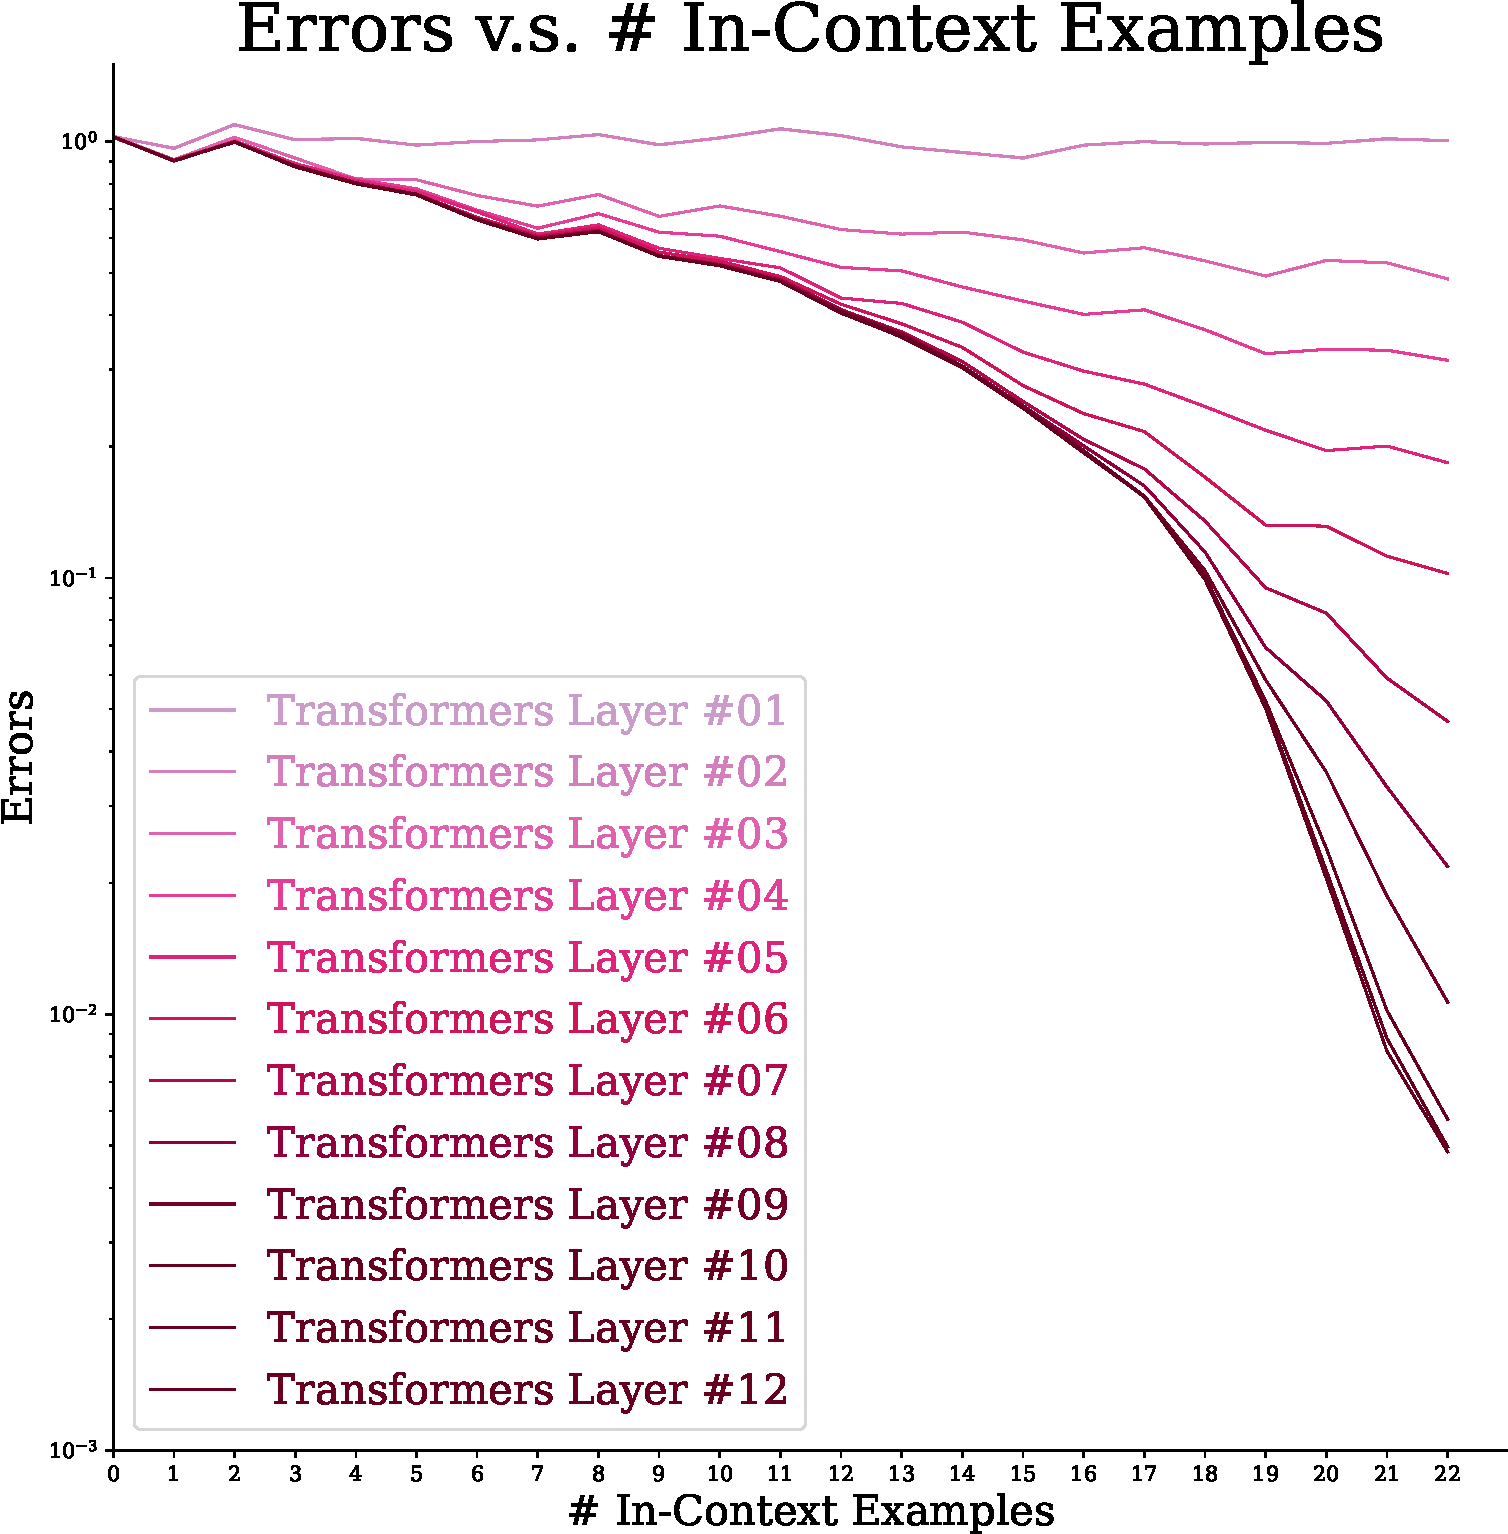
\includegraphics[width=0.31\linewidth]{Figures/progression/transformers.pdf} \label{subfig:transformers} } 
    \subfigure[Iterative Newton's Method]{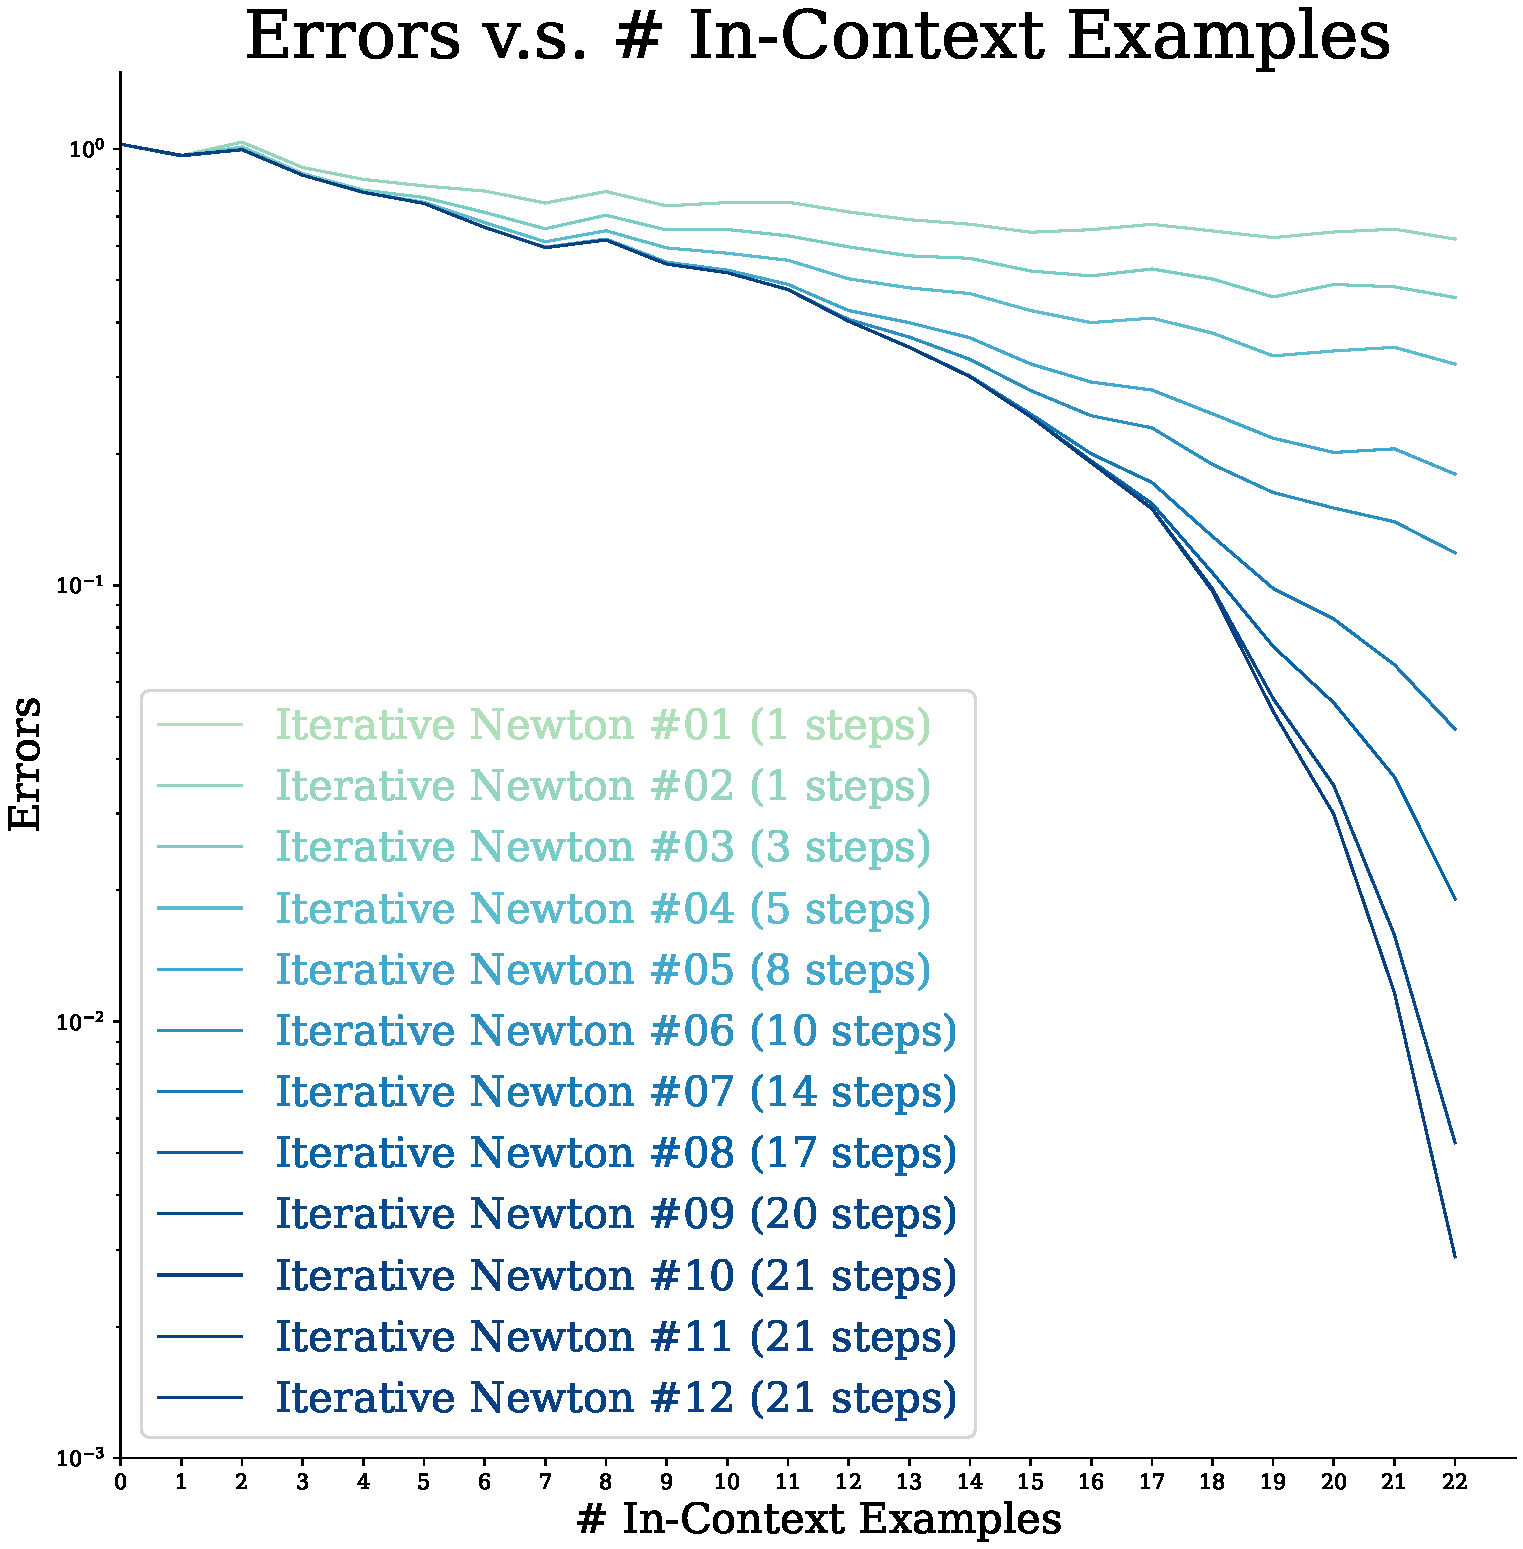
\includegraphics[width=0.31\linewidth]{Figures/progression/newton.pdf} \label{subfig:newton} } 
    \subfigure[LSTM]{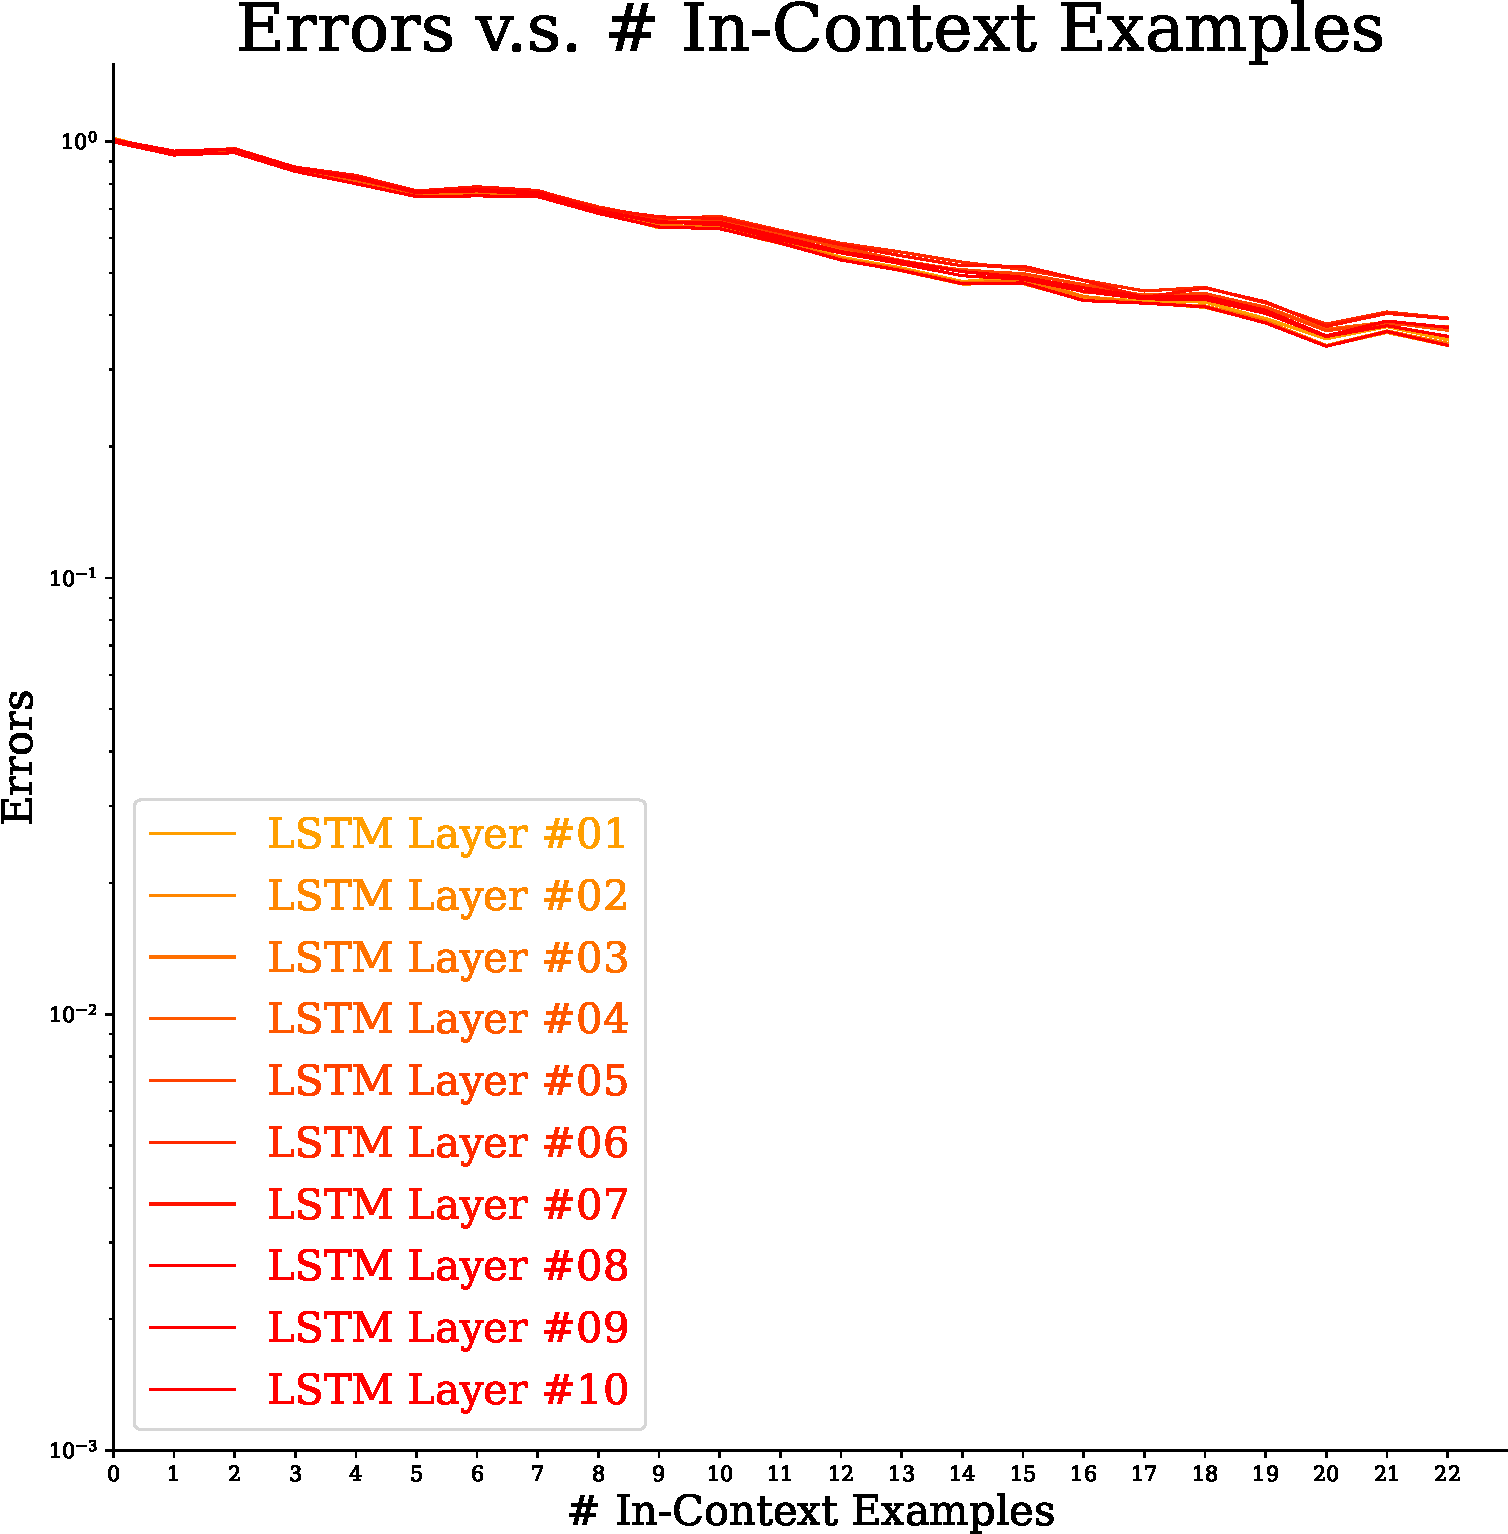
\includegraphics[width=0.31\linewidth]{Figures/progression/lstm.pdf} \label{subfig:lstm}}  \hfill
    \caption{\textbf{Progression of Algorithms.} (a) Transformer's performance improves over the layer index $\ell$. (b) \newton's performance improves over the number of iterations $k$, in a way that closely resembles the Transformer. We plot the best-matching $k$ to Transformer's $\ell$ following Definition \ref{def:matching}. (c) In contrast, LSTM's performance does not improve from layer to layer.}
    \vspace{-1.5ex}
    \label{fig:progression}
\end{figure*}
\subsubsection{Heatmaps} 
We present heatmaps with all values of similarities. 
\begin{figure}[!htp]
    \centering

\includegraphics[width=0.49\linewidth]{Figures/isotropic/resid_sim_heatmap_tf_newton_full.pdf}

\includegraphics[width=0.49\linewidth]{Figures/isotropic/resid_sim_heatmap_tf_gd_full.pdf}
\caption{\textbf{Similarity of Errors.} The best matching steps are highlighted in yellow.} \label{fig:full_heatmap_sim_e}
\end{figure}
\begin{figure}[!htp]
    \centering

\includegraphics[width=0.49\linewidth]{Figures/isotropic/w_sim_heatmap_tf_newton_full.pdf}

\includegraphics[width=0.49\linewidth]{Figures/isotropic/w_sim_heatmap_tf_gd_full.pdf}
\caption{\textbf{Similarity of Induced Weight Vectors.} The best matching steps are highlighted in yellow.} \label{fig:full_heatmap_sim_w}
\end{figure}

\begin{figure}[!htp]
    \centering
    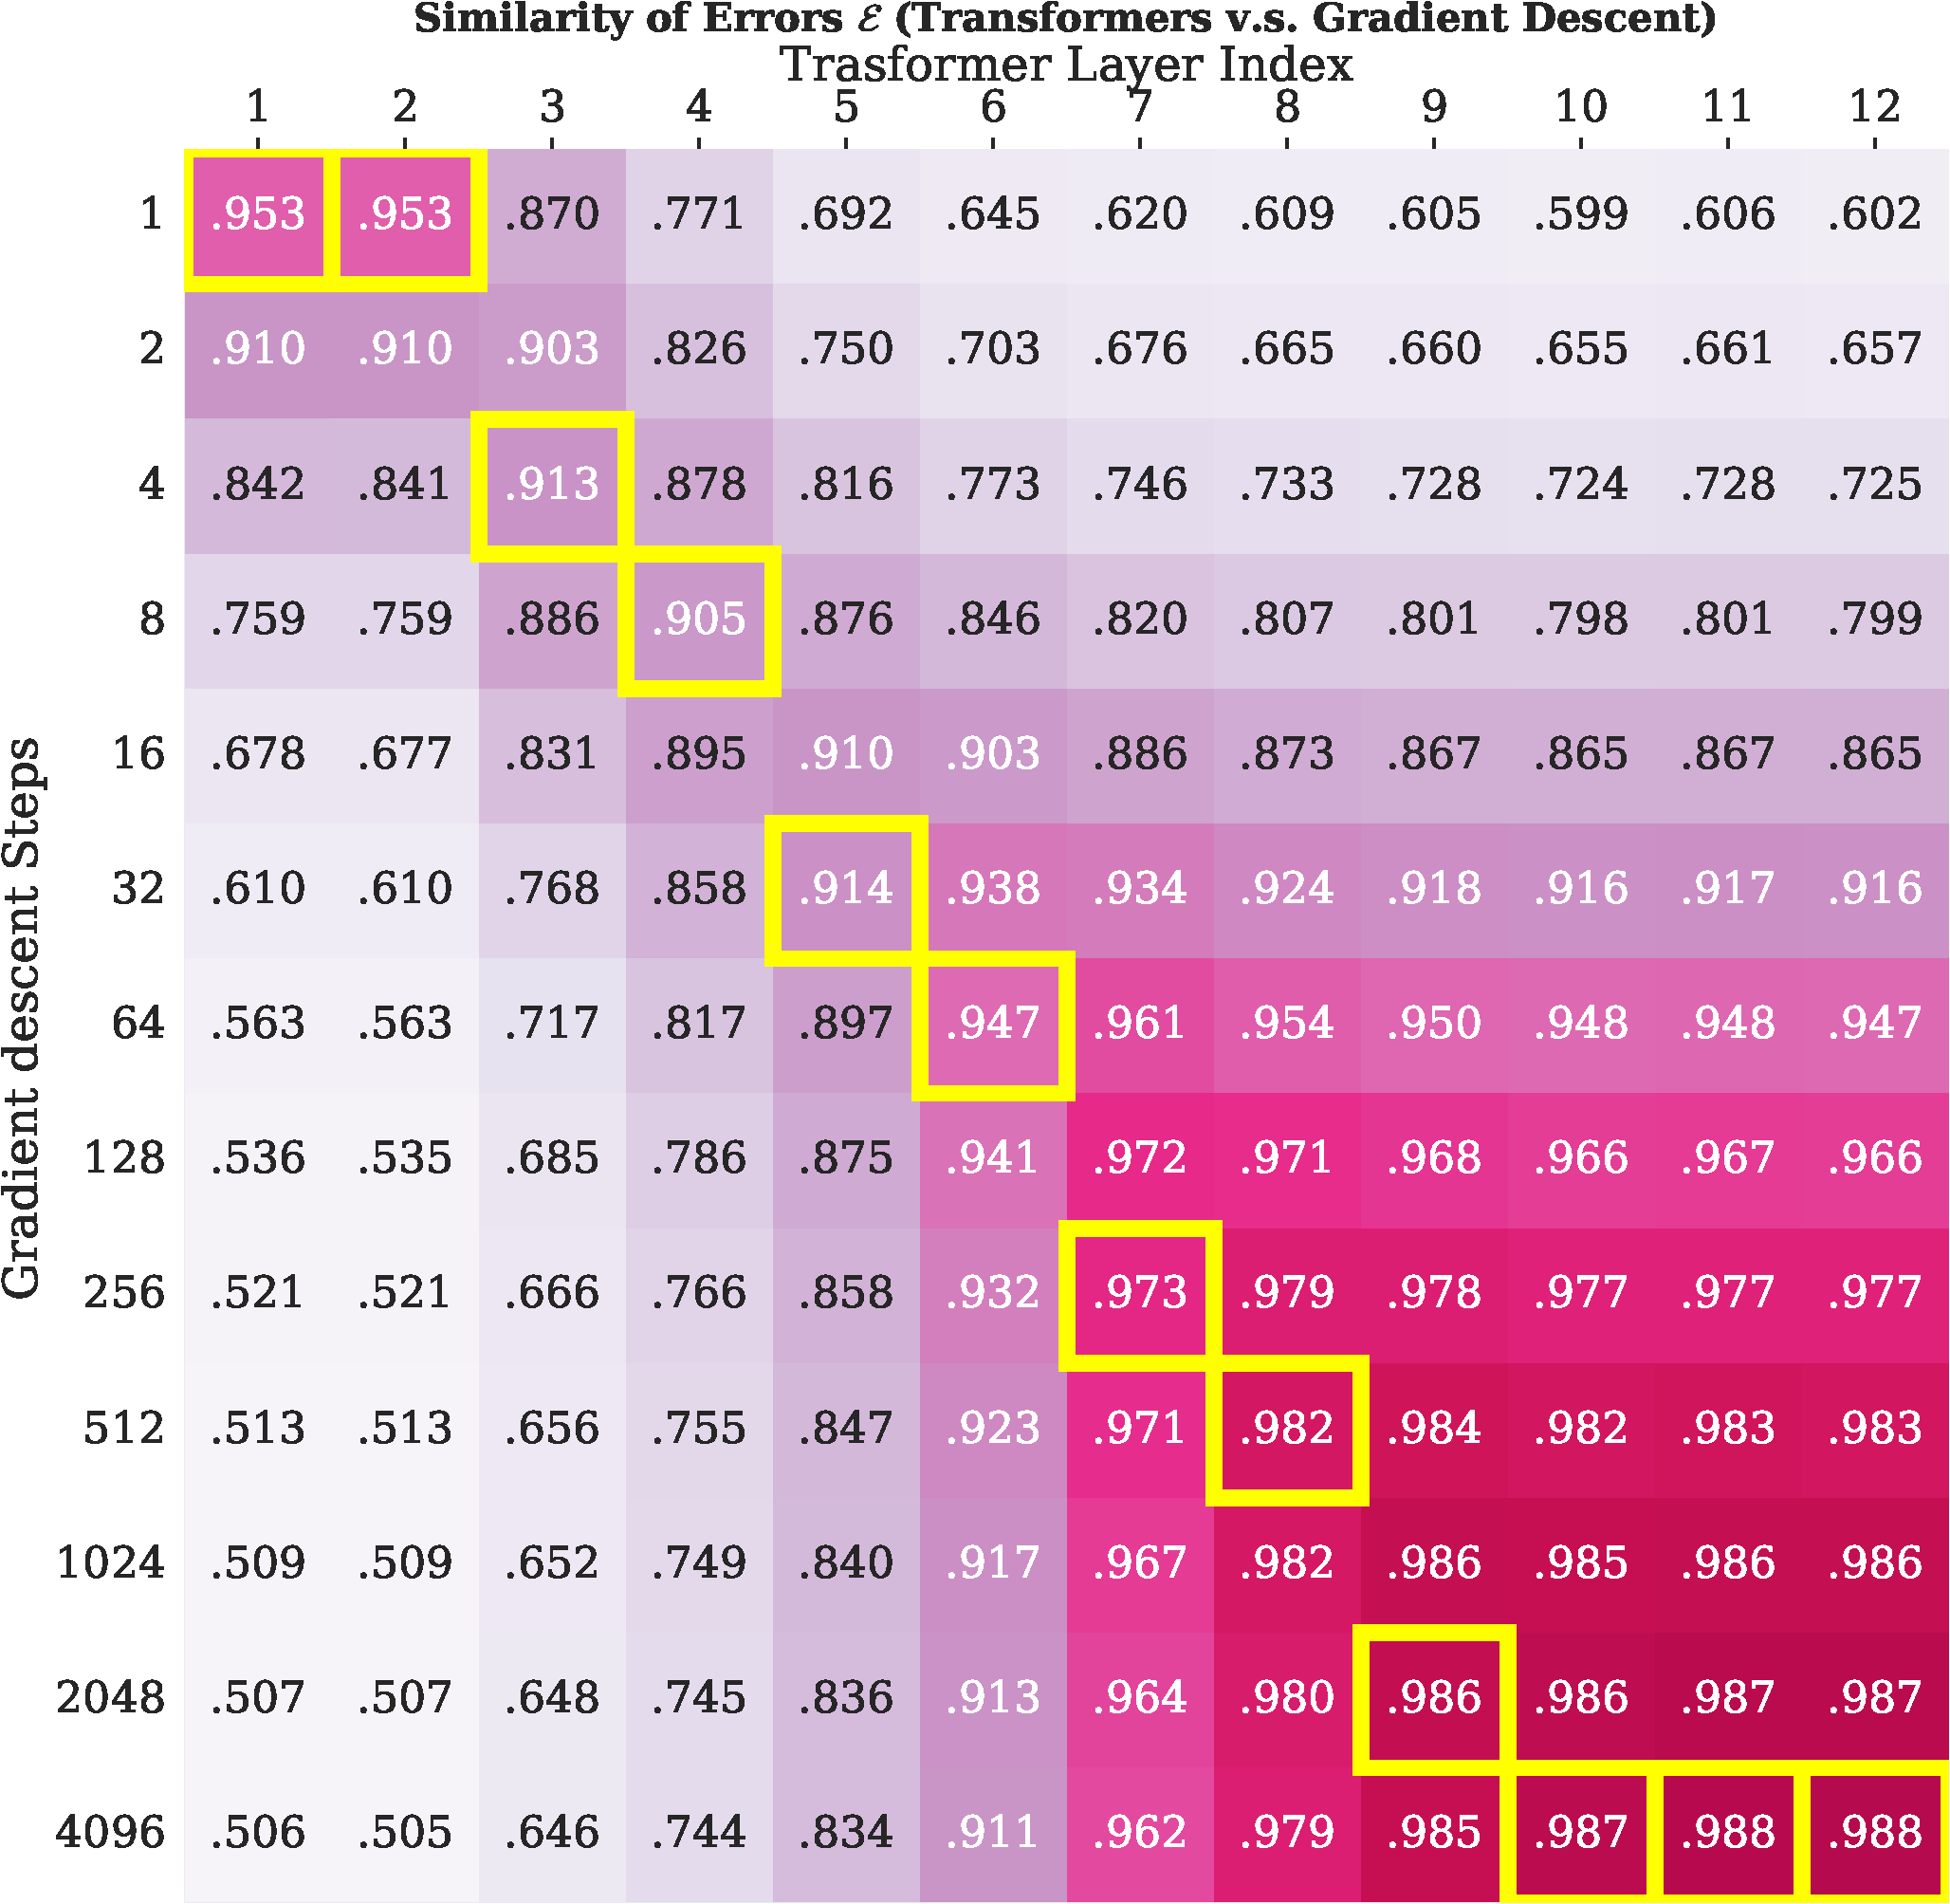
\includegraphics[width=0.7\linewidth]{Figures/isotropic/exponential/resid_sim_heatmap_tf_gd_exp_full.pdf}
    \caption{\textbf{Similarity of Errors of Gradient Descent in Log Scale.} The best matching steps are highlighted in yellow. Putting the number of steps of \gd\ in log scale further verifies the claim that Transformer's rate of covergence is exponentially faster than that of \gd.}
    \label{fig:gd_heatmap_log_scale}
\end{figure}

\clearpage
\subsubsection{Comparison with Other Second-Order Methods} \label{sec:second-order}

In this section, we ablate with alternative second-order methods, such as Conjugate Gradient, BFGS, and its limited memory variant, L-BFGS. 

\paragraph{Conjugate Gradient Method. } For linear regression problems, the Conjugate Gradient (CG) method solves the linear system
$$
\underbrace{(\bX^\top \bX)}_{\bS} \bw - \bX^\top \by = 0
$$
CG finds the weight vector $\hat{\bw}^{CG}$ with initialization $\bw_0$ by maintain a set of conjugate gradient $\{\Delta \bw_1, \cdots, \Delta \bw_k\}$. It follows the iterative update rule
\begin{equation}
    \begin{aligned}
        & \bd_k = - \nabla \mathcal L(\bw_k) \\
        & \Delta \bw_k = \bd_k - \sum_{i=0}^{k-1} \frac{\bd_k^\top \bS \Delta \bw_i}{\Delta \bw_i^\top \bS \Delta \bw_i} \Delta \bw_i \\
        & \alpha_k = \arg \min_{\alpha} \mathcal L(\bw_k + \alpha \Delta \bw_k) \\
        &\bw_{k+1} = \bw_k + \alpha_k \Delta \bw_k
    \end{aligned}
\end{equation}

The conjugate Gradient method requires $\mathcal O\left(\sqrt{\kappa} \log(1/\epsilon)\right)$ steps to converge to an $\epsilon$ error on quadratic objectives such as linear regression. 

\paragraph{BFGS. } Broyden– Fletcher–Goldfarb–Shanno (BFGS) is a Quasi-Newton method, designed to approximate the inverse Hessian $\bB_k :\approx \nabla^2 \mathcal L(\bw_k)^{-1}$. The BFGS updates are given by
\begin{equation}
    \bw_{k+1} = \bw_k - \alpha_k \bB_k \nabla \mathcal L(\bw_k)
\end{equation}
where 
\begin{equation*}
    \begin{aligned}
    \bs_k &= \bw_{k+1} - \bw_k \\
    \by_k &= \nabla \mathcal L(\bw_{k+1}) - \nabla \mathcal L(\bw_{k}) \\
    \bB_{k+1} &= \bB_k - \frac{\bB_k \by_k \by_k^\top \bB_k}{\by_k^\top \bB_k \by_k} + \frac{\bs_k \bs_k^\top}{\by_k^\top \bs_k}
    \end{aligned}
\end{equation*}
When $k$ is large, $\bB_k$ approximates the inverse Hessian well.

\paragraph{L(imited-memory)-BFGS.} L-BFGS is a limited-memory version of BFGS. Instead of the inverse Hessian $\bB_k$, L-BFGS maintains a history of past $m$ updates (where $m$ is usually small). Recall the iterative update rule of $\bB_k$ in BFGS
\begin{equation}
    \bB_{k+1} = \bB_k - \frac{\bB_k \by_k \by_k^\top \bB_k}{\by_k^\top \bB_k \by_k} + \frac{\bs_k \bs_k^\top}{\by_k^\top \bs_k}
\end{equation}
Unlike BFGS, which recursively unroll to an initialization $\bB_0$, L-BFGS only unroll to $\bB_{k-m}$ but replacing $\bB_{k-m}$ with $\bB_\mathrm{init}$. In this regard, running $n$ steps of L-BFGS only requires $\mathcal O(mn)$ memory, which is more memory-efficient than BFGS who requires $\mathcal O(n^2)$ memory. The trade-off is that L-BFGS won't have a good estimate of the inverse Hessian when $m < d$, where $d$ is the dimensionality of the quadratic problem. In this regard, it will converge slower than full BFGS. 

In \Cref{fig:bfgs} and \Cref{fig:conjugate-gradient}, we compare Transformers with BFGS, L-BFGS, and Conjugate Gradient method on the metric of similarity of errors. We find that Transformers have a similar \textit{linear} correspondence with BFGS. This is perhaps not surprising, given that BFGS also gets a superlinear convergence rate for linear regression \cite{nocedal1999numerical}. Meanwhile, Transformers show a substantially faster convergence rate than L-BFGS and CG.


\begin{figure}[!htp]
    \centering
    \subfigure[Transformer v.s. BFGS]{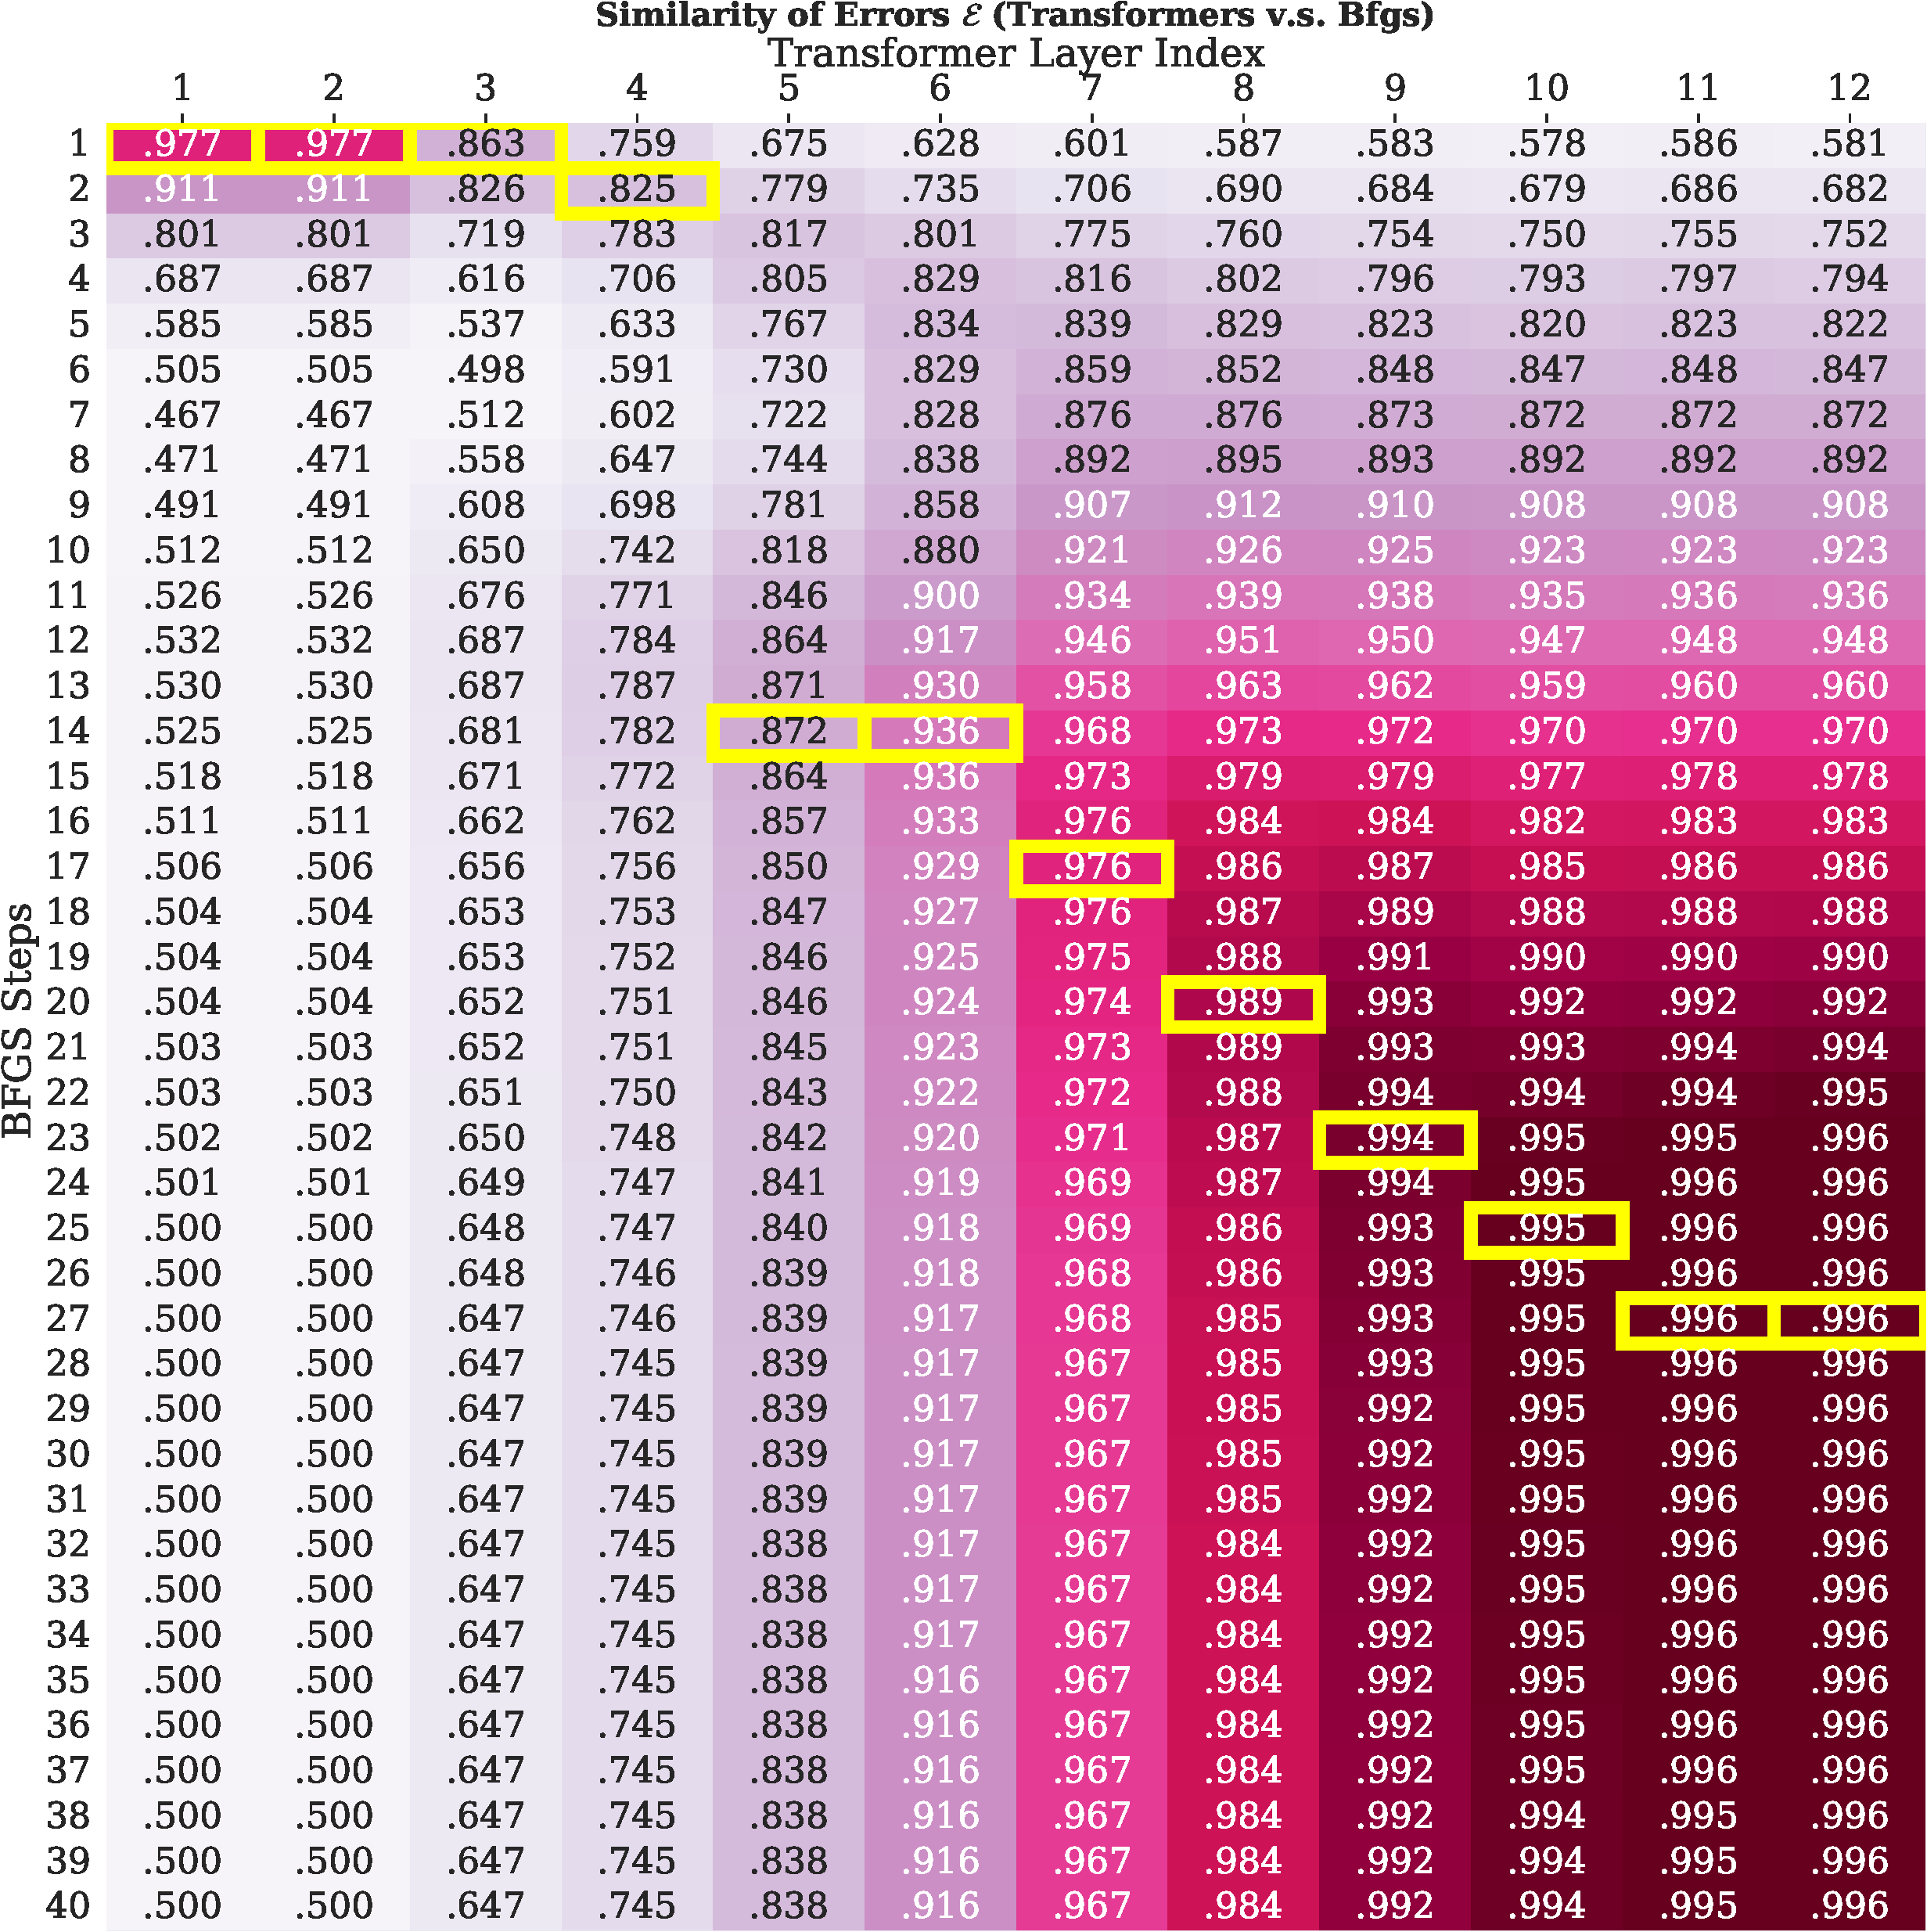
\includegraphics[width=0.48\linewidth]{Figures/quasi_newton/resid_sim_heatmap_tf_bfgs_full.pdf}}
    \subfigure[Transformer v.s. L-BFGS]{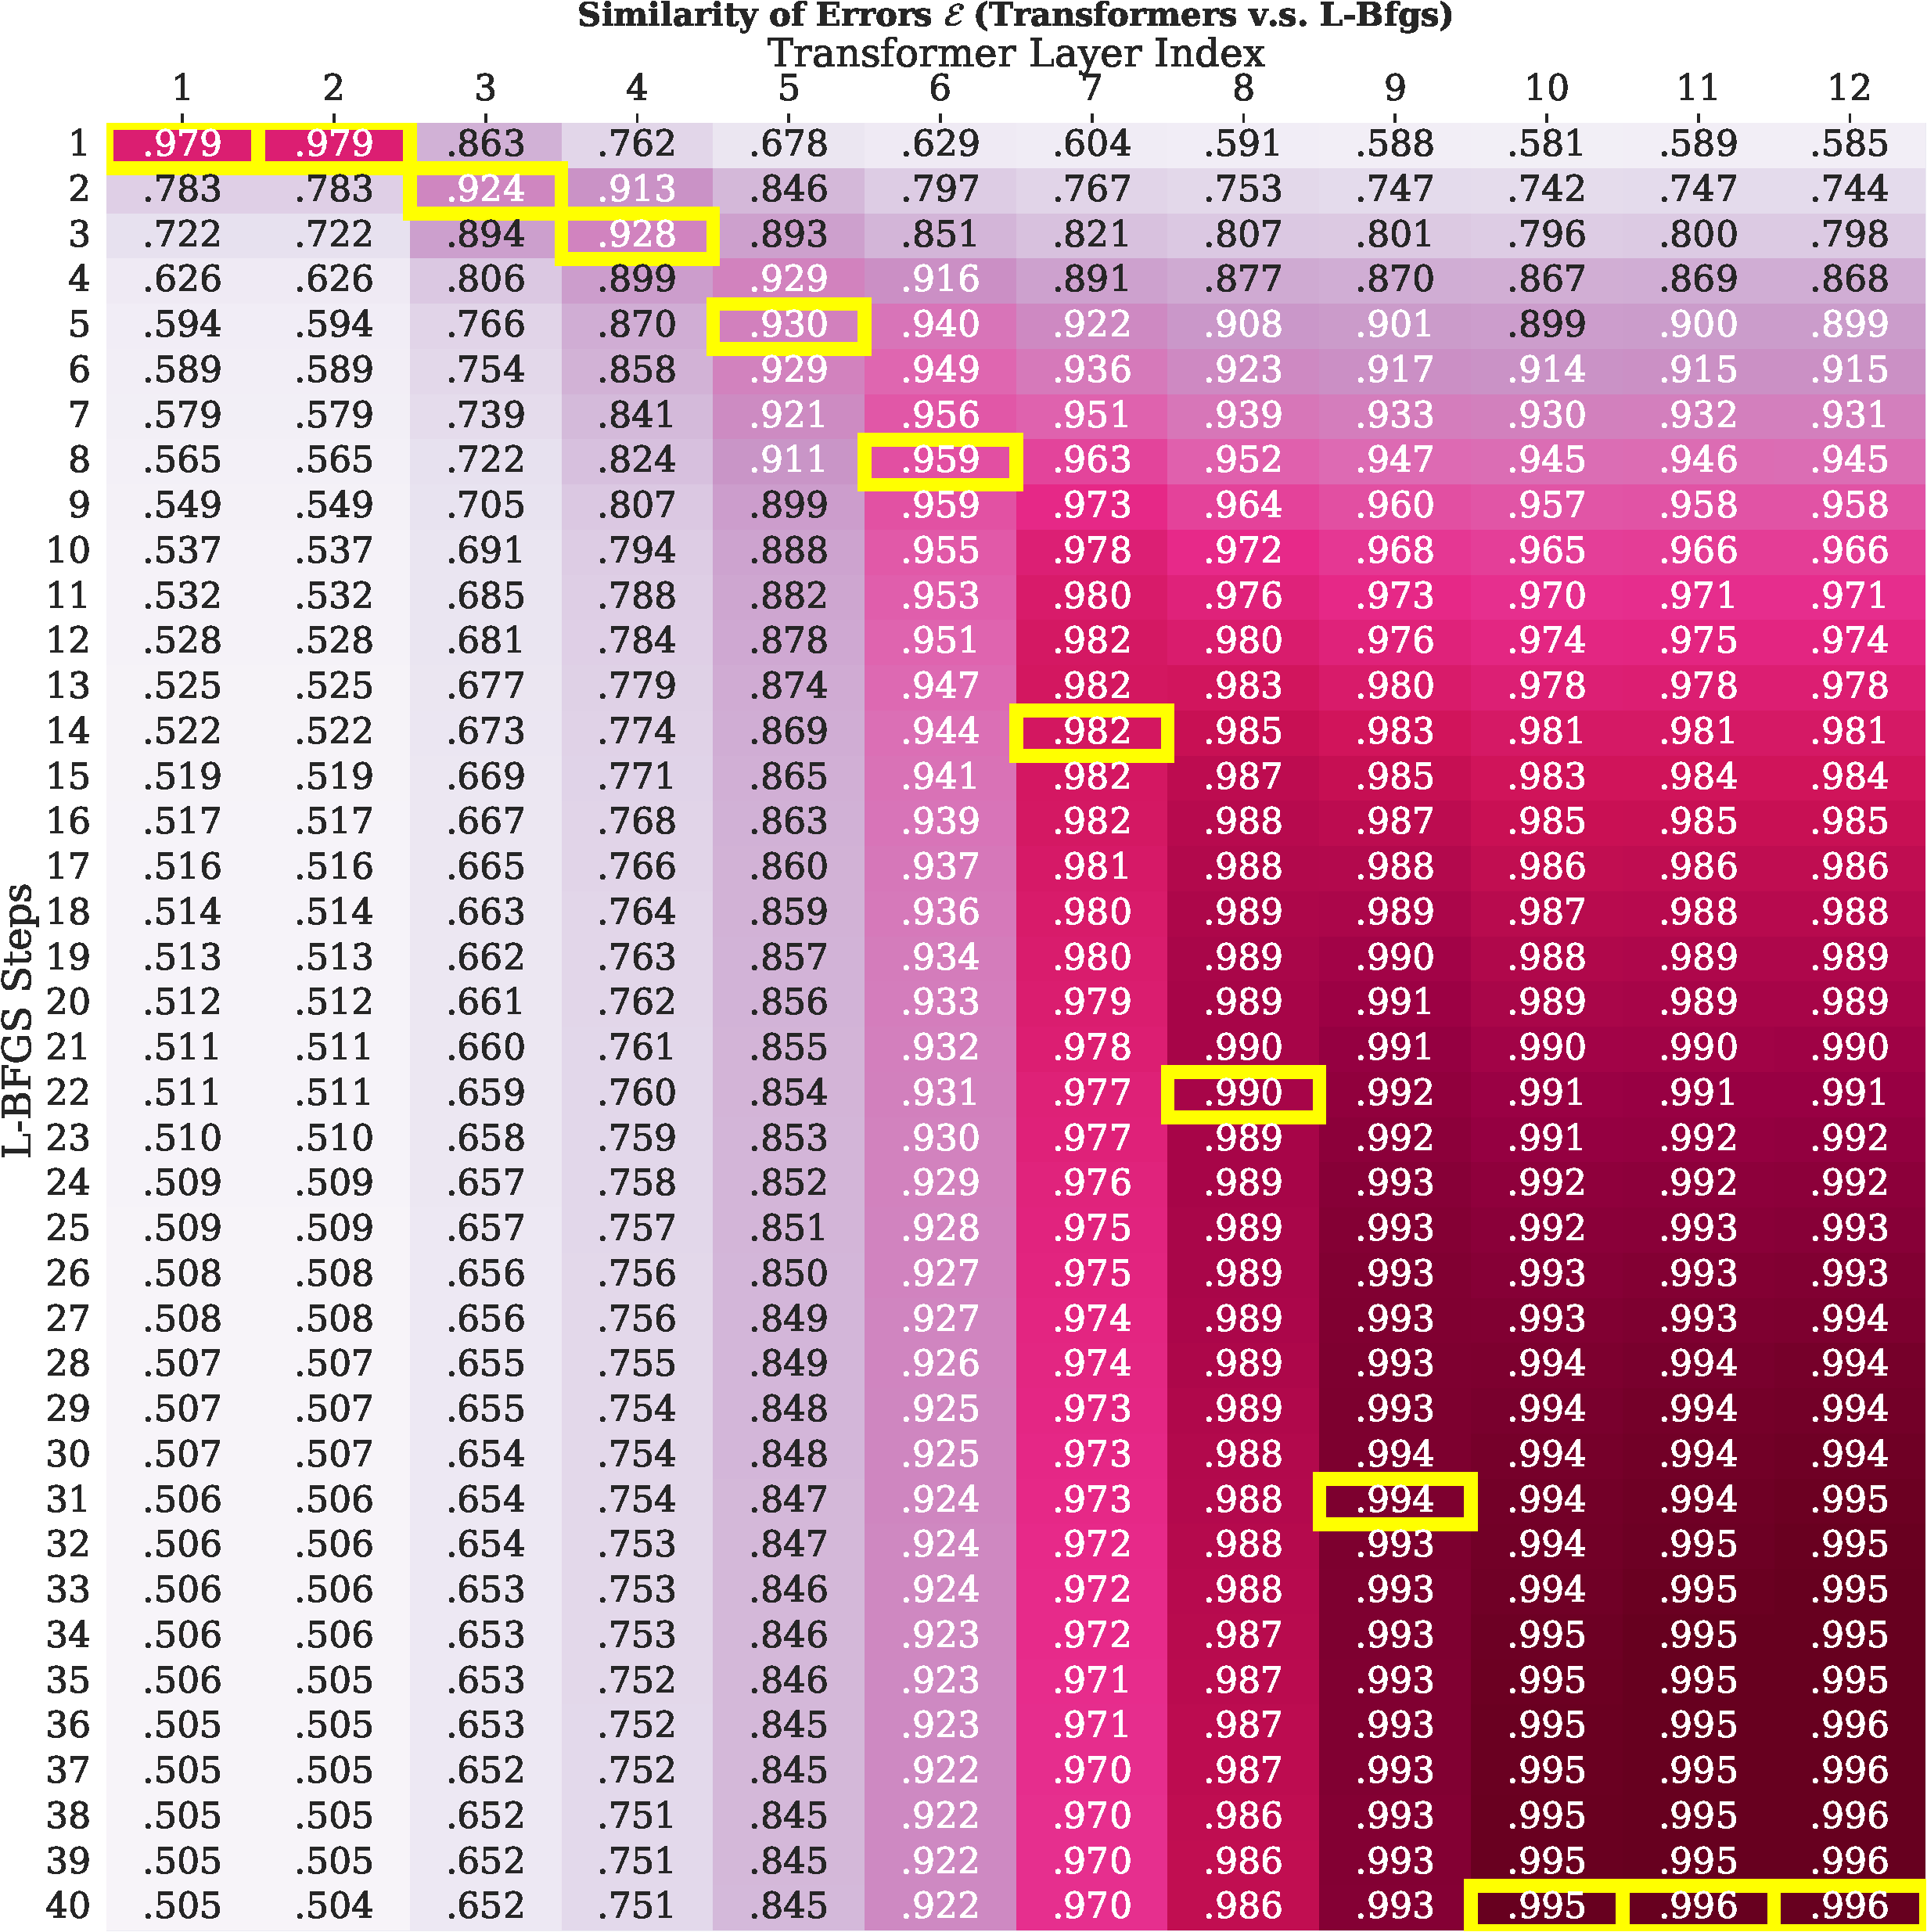
\includegraphics[width=0.48\linewidth]{Figures/quasi_newton/resid_sim_heatmap_tf_l-bfgs_full.pdf}}
    \caption{\textbf{Similarity of Errors between Transformers and BFGS or L-BFGS.} The best matching steps are highlighted in yellow. We find that Transformer, from layers 6 to 11, has a linear correspondence with BFGS. For L-BFGS, due to its limited memory, it approximates second-order information more slowly and results in a slower convergence rate than Transformers.}
    \label{fig:bfgs}
\end{figure}

\begin{figure}[!htp]
    \centering
    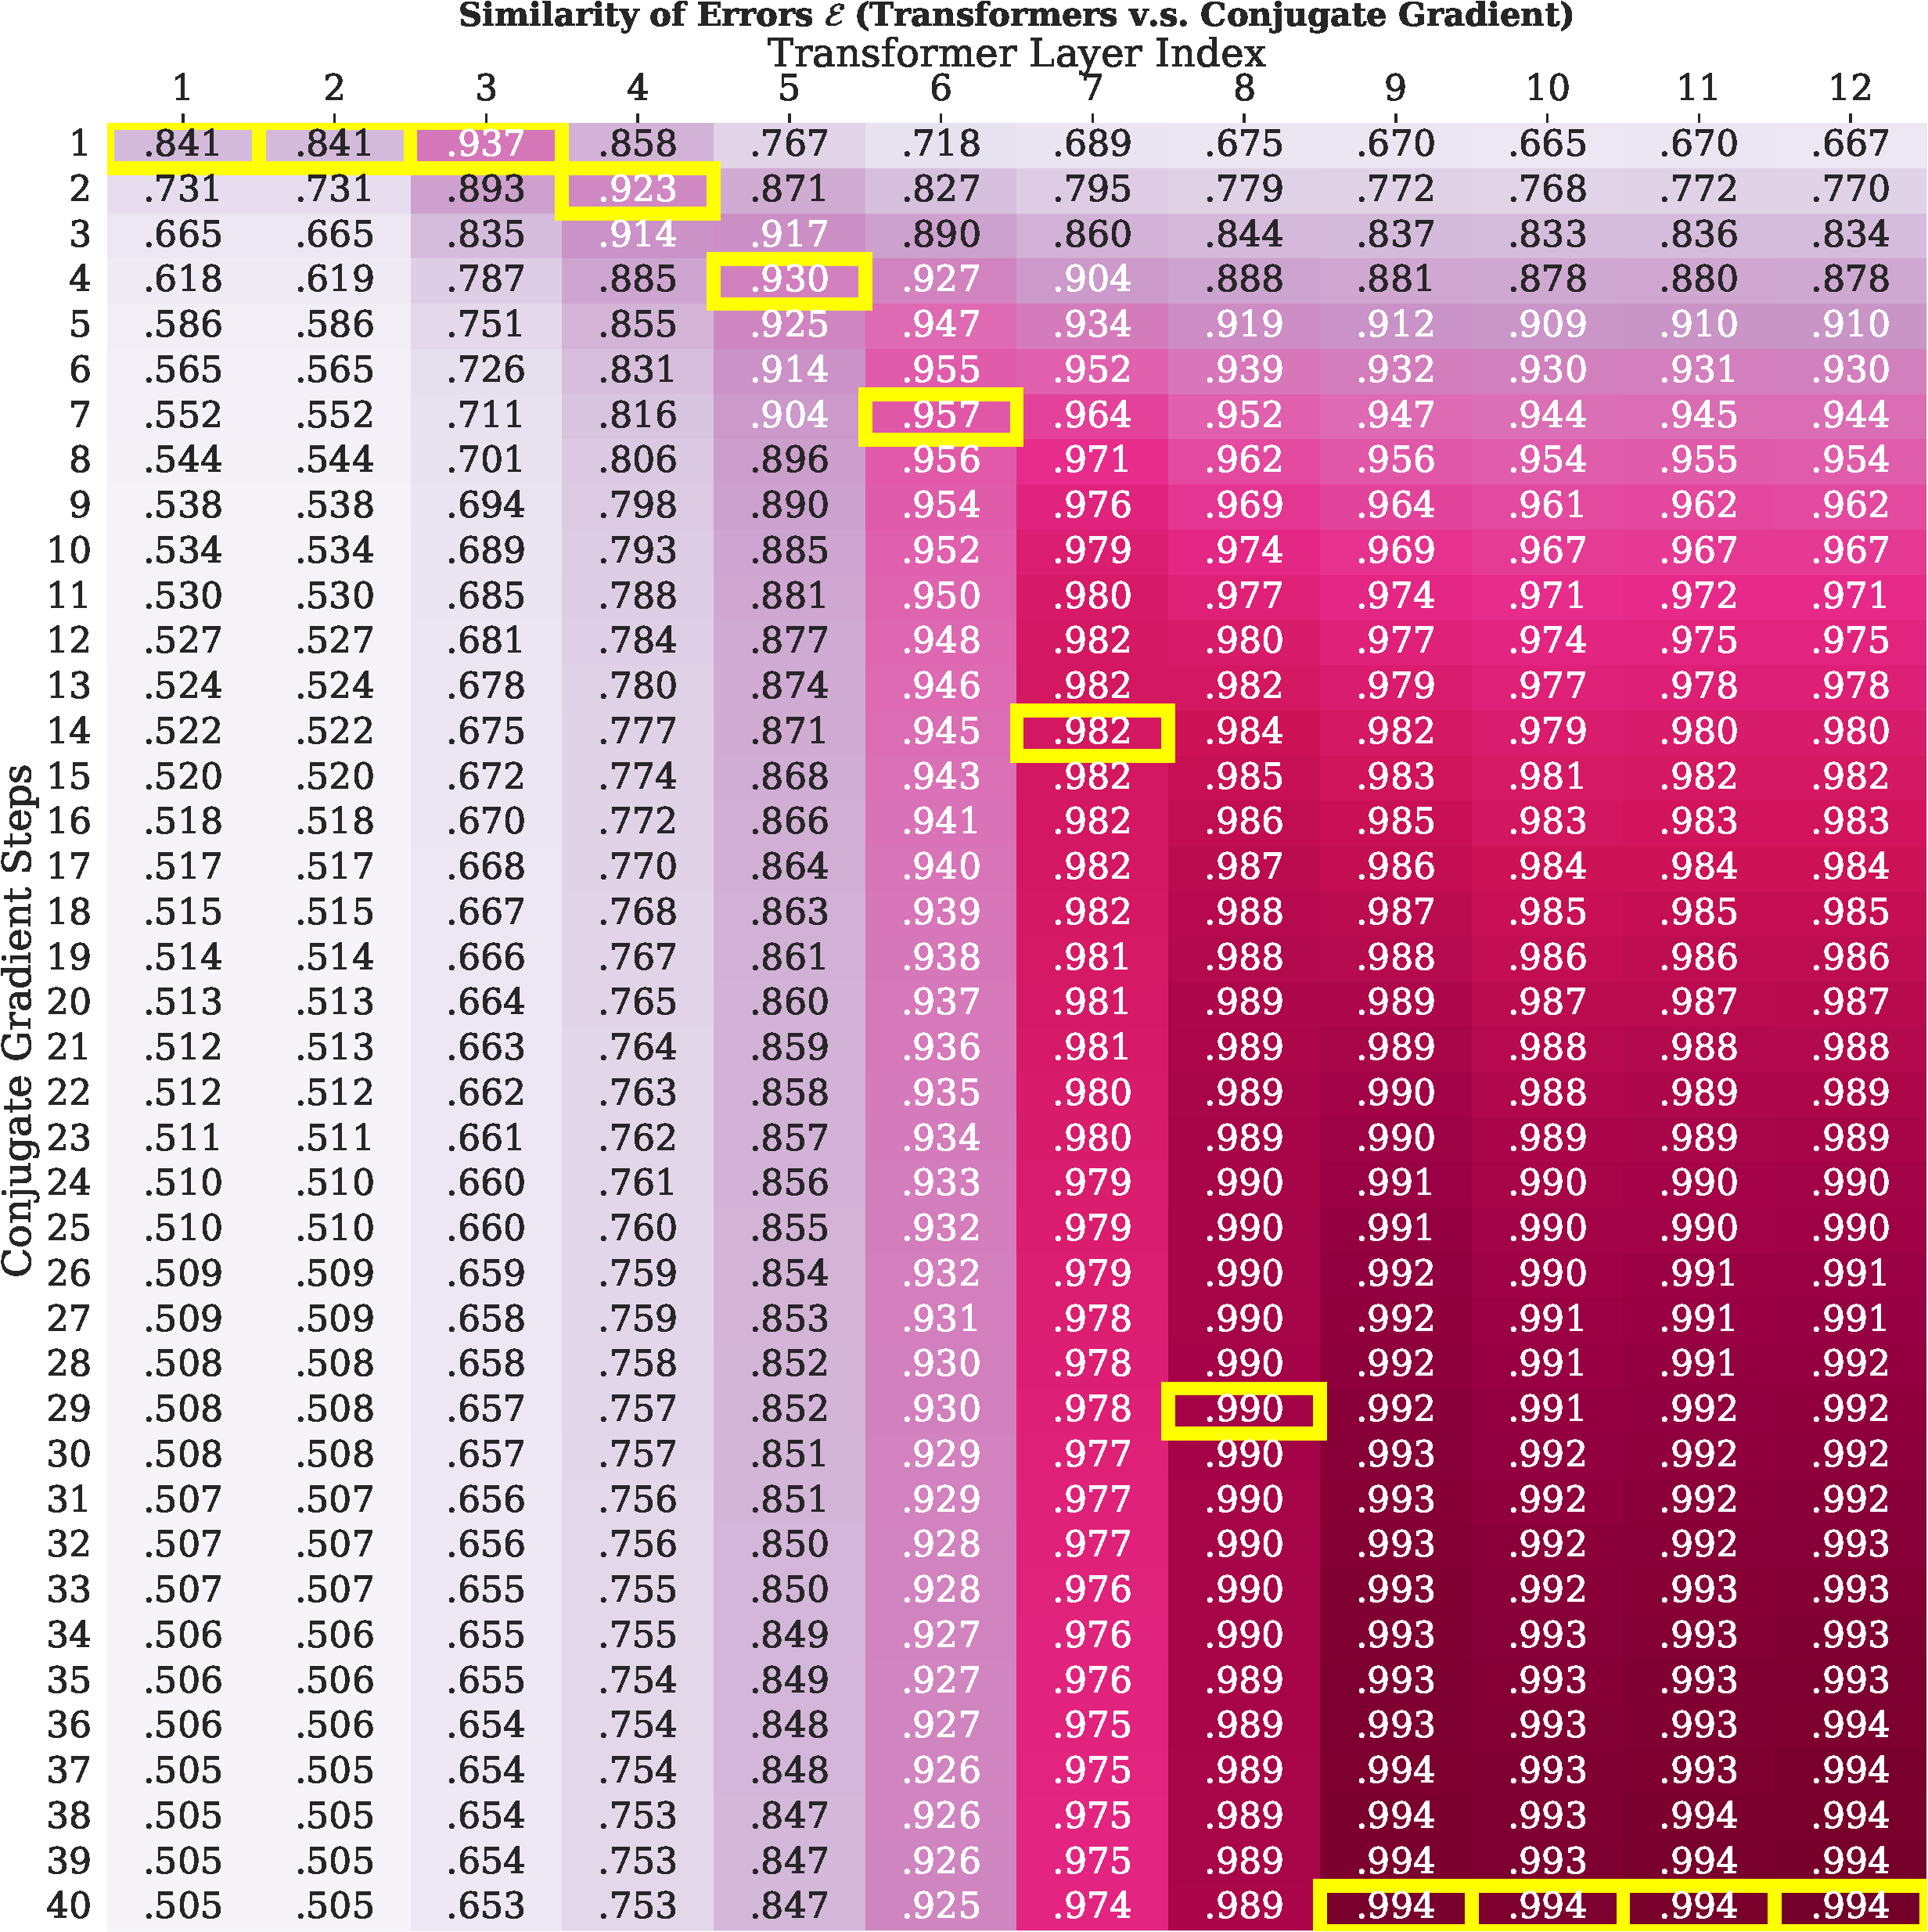
\includegraphics[width=0.55\linewidth]{Figures/quasi_newton/resid_sim_heatmap_tf_conjugate_gradient_full.pdf}
    \caption{\textbf{Similarity of Errors between Transformers and Conjugate Gradient.} Transformer's convergence rate is still faster than conjugate gradient methods. }
    \label{fig:conjugate-gradient}
\end{figure}

\clearpage
\subsubsection{Additional Results on Comparison over Transformer Layers}
\begin{figure}[!htp]
\centering
\subfigure[Similarity of Errors]{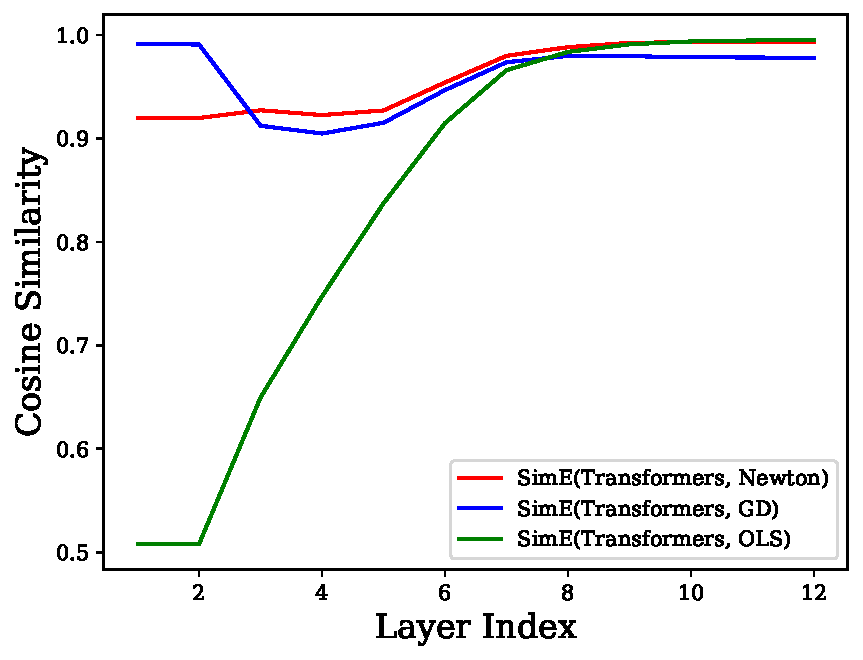
\includegraphics[width=0.4\linewidth]{Figures/over_layers/residual_over_layers.pdf}}\label{fig:over_layer_sim_e}
\subfigure[Similarity of Induced Weights]{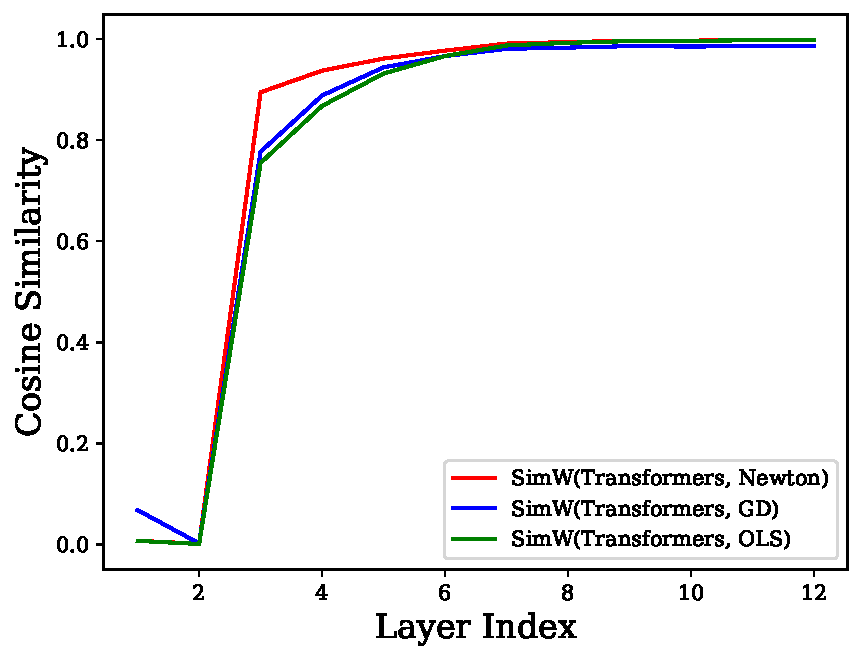
\includegraphics[width=0.4\linewidth]{Figures/over_layers/induced_w_over_layers.pdf}} \label{fig:over_layer_sim_w}
% \begin{subfigure}{}
%   \centering
%   \caption{Similarity of Errors}
%   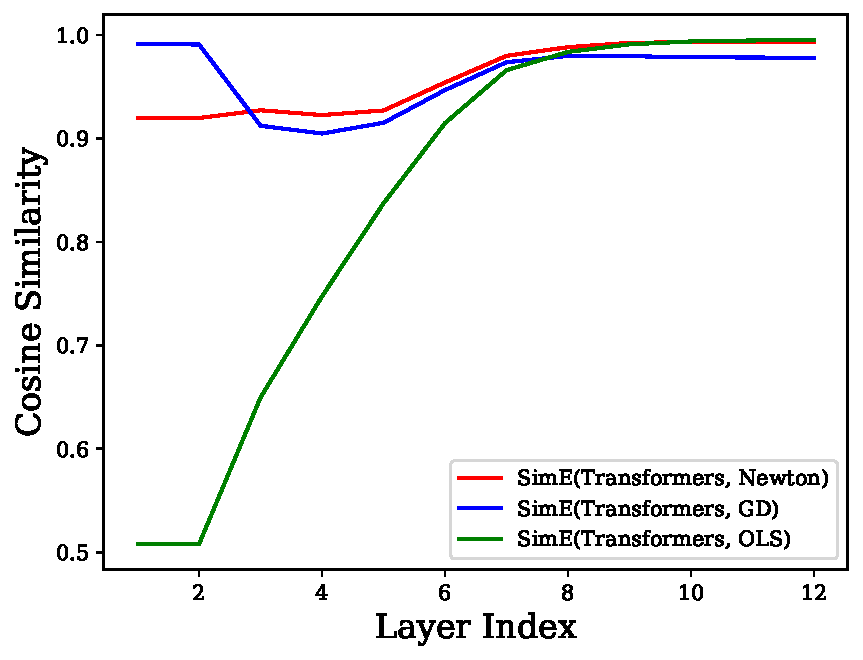
\includegraphics[width=0.4\linewidth]{Figures/over_layers/residual_over_layers.pdf}
%   \label{fig:over_layer_sim_e}
% \end{subfigure}   
% \begin{subfigure}{}
%   \centering
%   \caption{Similarity of Induced Weights}
%   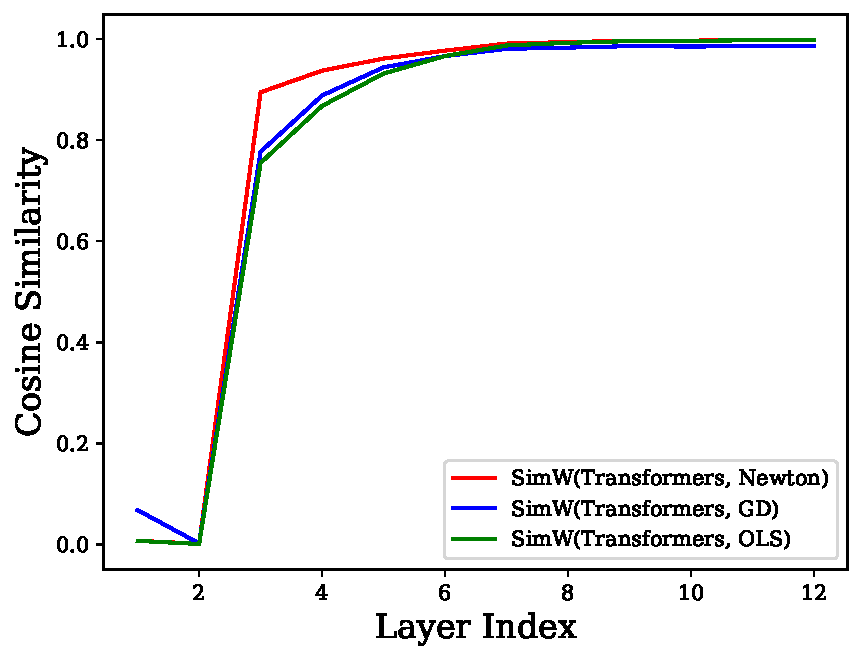
\includegraphics[width=0.4\linewidth]{Figures/over_layers/induced_w_over_layers.pdf}
%   \label{fig:over_layer_sim_w}
% \end{subfigure}
  \caption{Similarities between Transformer and candidate algorithms. Transformers resemble \textit{Iterative Newton's Method} the most.}
  \label{fig:over_layers}
\end{figure}

\subsubsection{Additional Results on Similarity of Induced Weights} \label{app:sim_w}
We present more details line plots for how the similarity of weights changes as the models see more in-context observations $\{\bx_i, y_i\}_{i=1}^n$, i.e., as $n$ increases. We fix the number of Transformers layers $\ell$ and compare with other algorithms with their best-match steps to $\ell$ in \Cref{fig:over_examples}. 

\begin{figure}[hb]
    \centering
    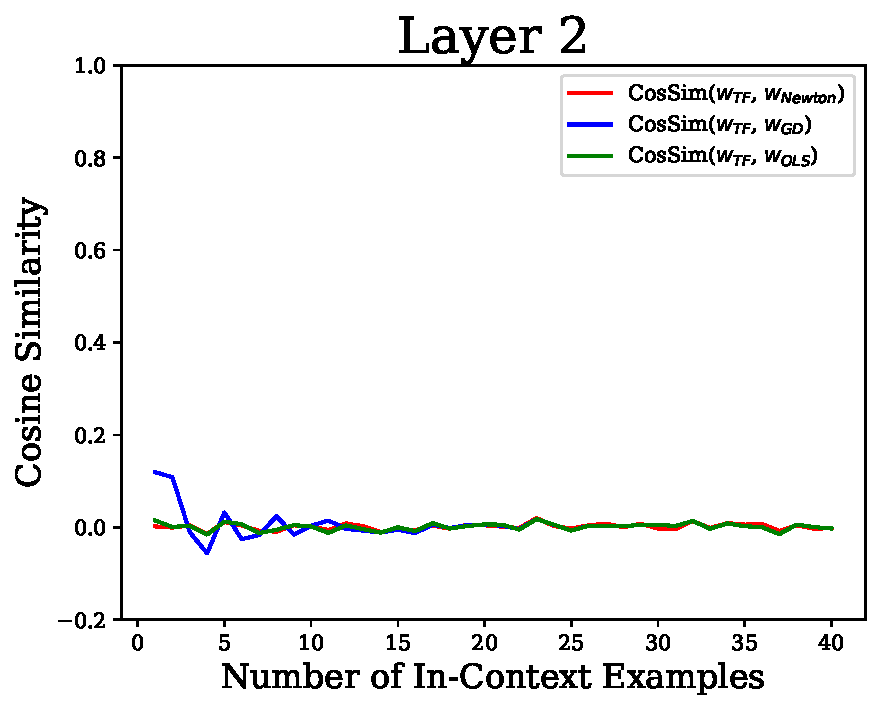
\includegraphics[width=0.32\linewidth]{Figures/over_examples/over_examples_layer_2.pdf}
    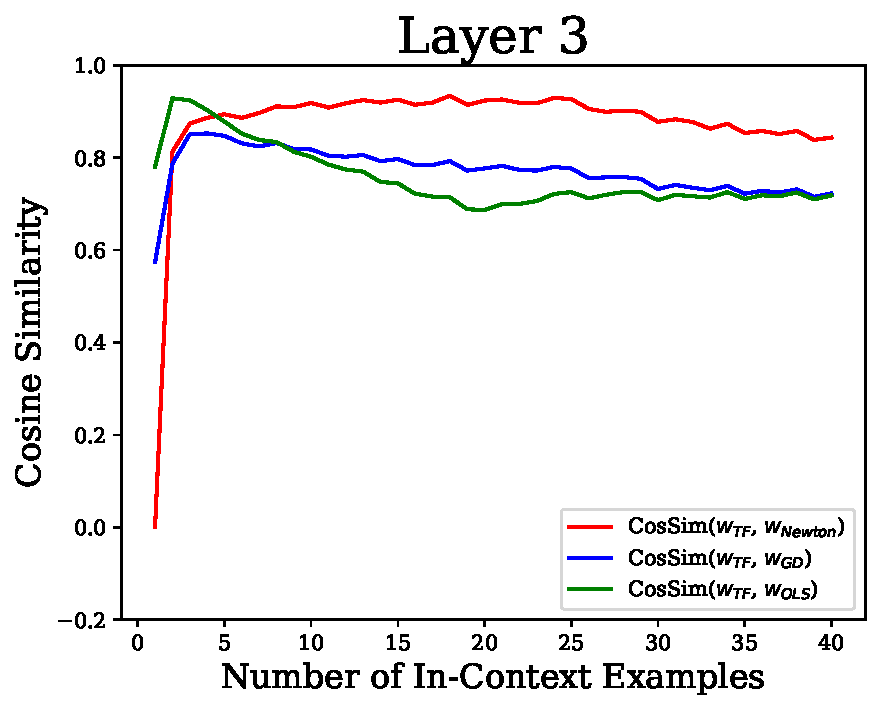
\includegraphics[width=0.32\linewidth]{Figures/over_examples/over_examples_layer_3.pdf}
    % 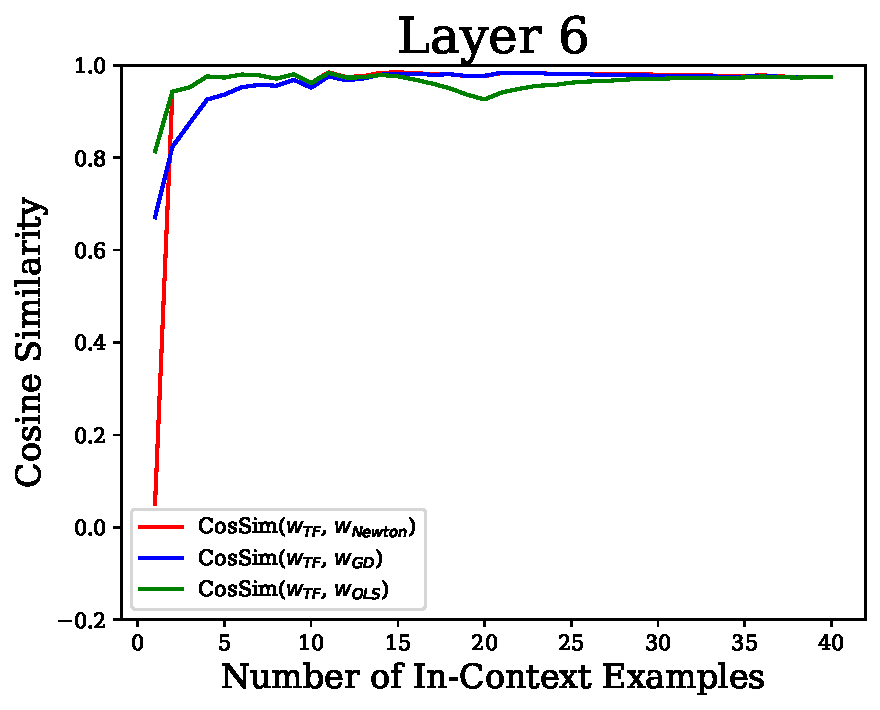
\includegraphics[width=0.24\linewidth]{Figures/over_examples/over_examples_layer_6.pdf}
    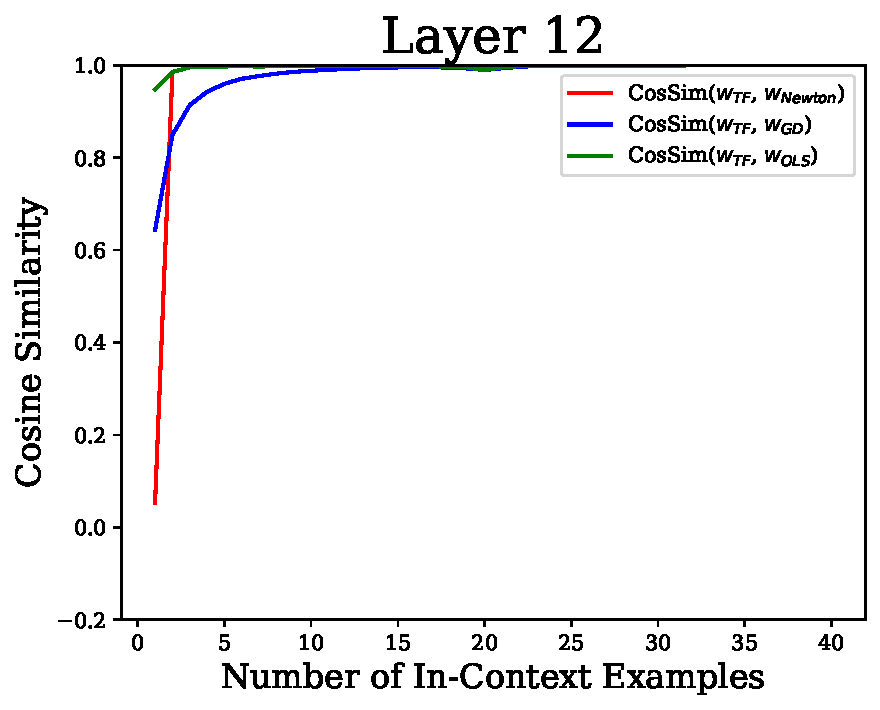
\includegraphics[width=0.32\linewidth]{Figures/over_examples/over_examples_layer_12.pdf}
    \caption{\textit{Similarity of induced weights} over varying number of in-context examples, on three layer indices of Transformers, indexed as 2, 3 and 12. We find that initially at layer 2, the Transformers model hasn't learned so it has zero similarity to all candidate algorithms. As we progress to the next layer number 3, we find that Transformers start to learn, and when provided few examples, Transformers are more similar to OLS but soon become most similar to the Iterative Newton's Method. Layer  12 shows that Transformers in the later layers converge to the OLS solution when provided more than 1 example. We also find there is a dip around $n = d$ for similarity between Transformers and OLS but not for Transformers and Newton, and this is probably because OLS has a more prominent double-descent phenomenon than Transformers and Newton.}
    \label{fig:over_examples}
\end{figure}

\clearpage
\subsection{Varying Data Distribution or Function Class}
\subsubsection{Experiments on Ill-Conditioned Problems}\label{app:ill}
In this section, we repeat the same experiments as we did on isotropic data in the main text and in \Cref{app:exp_standard}, and we change the covariance matrix to be ill-conditioned such that $\kappa(\bSigma) = 100$. 
\begin{figure}[htp]
    \centering
    \subfigure[Transformers]{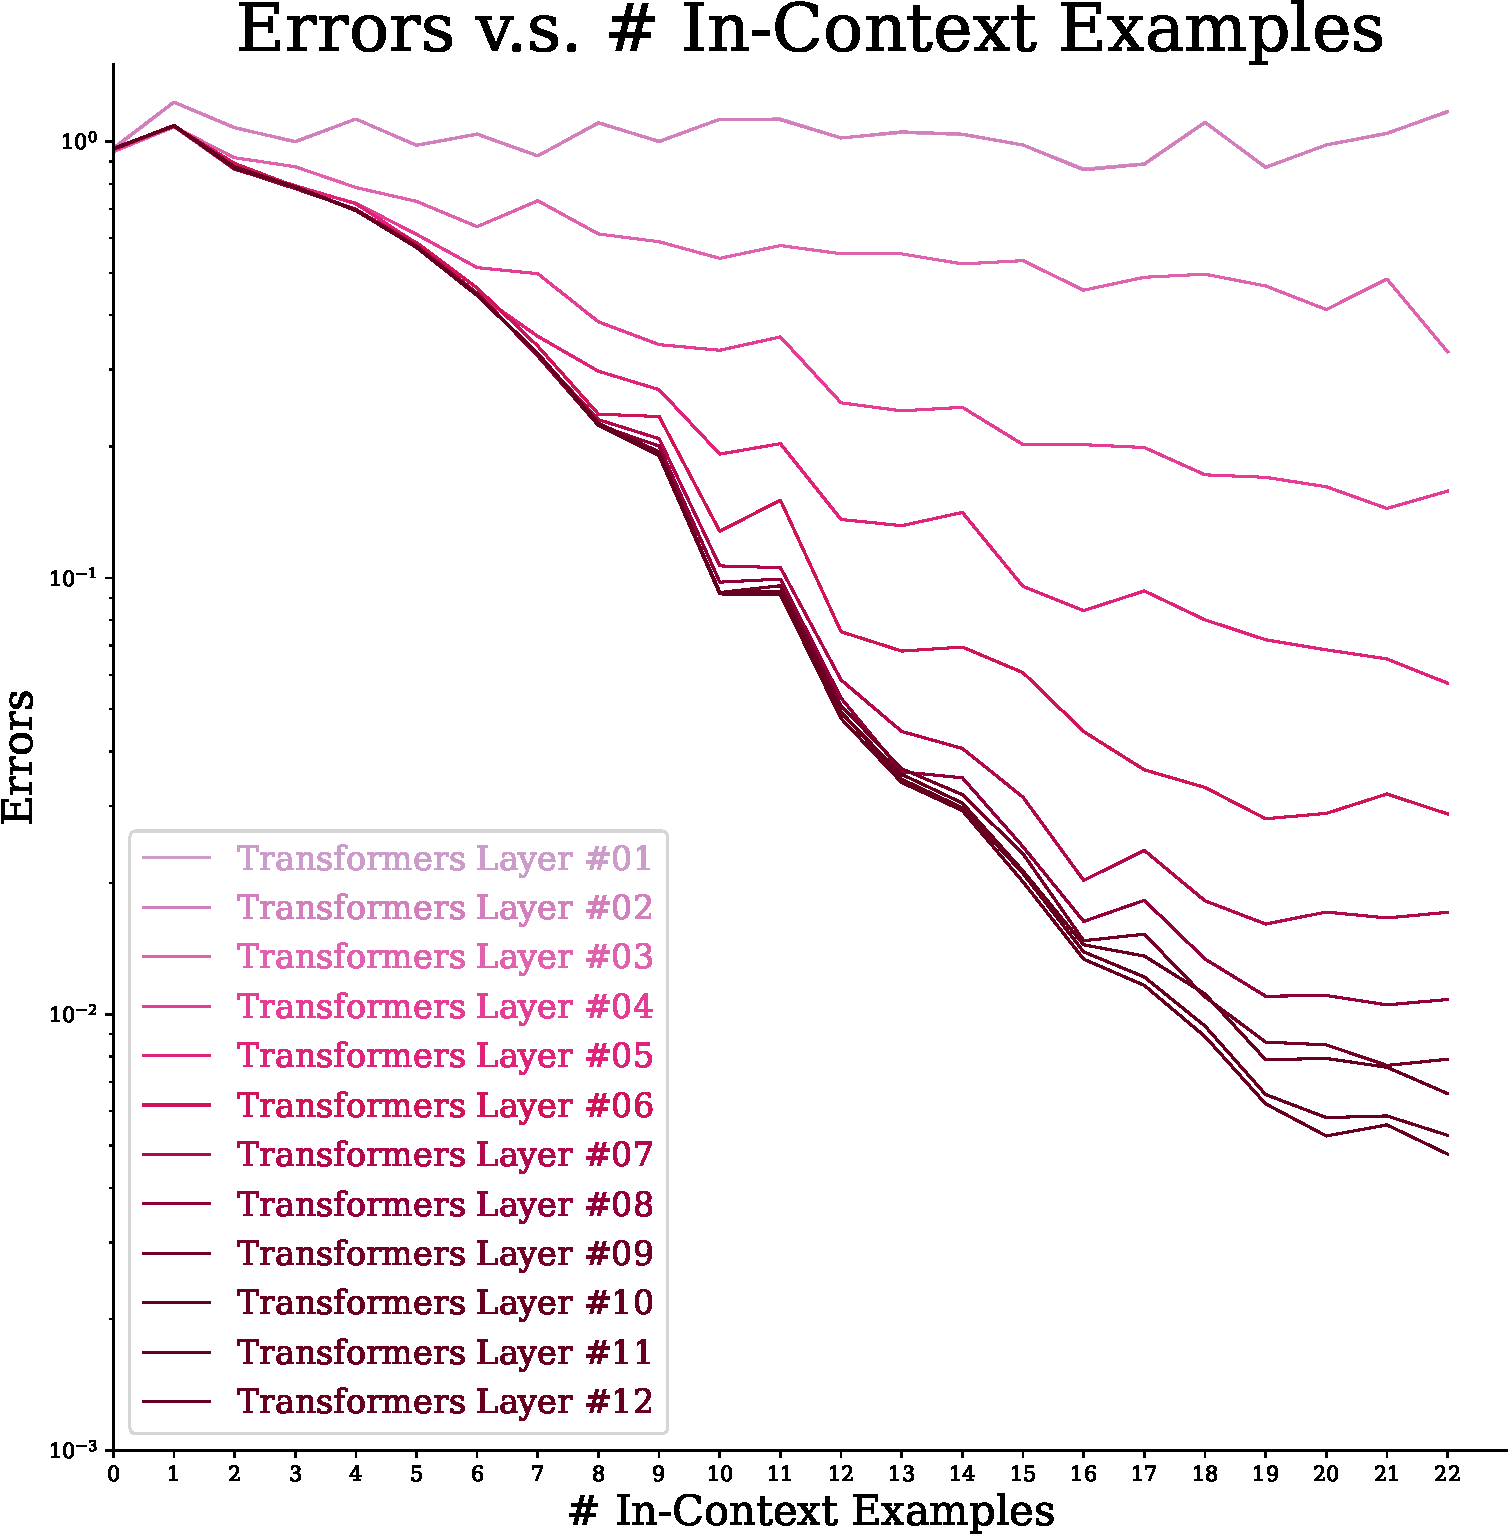
\includegraphics[width=0.4\linewidth]{Figures/progression/transformers_skew_only.pdf}} \label{subfig:transformers_skew_only}
    \subfigure[Iterative Newton's Method]{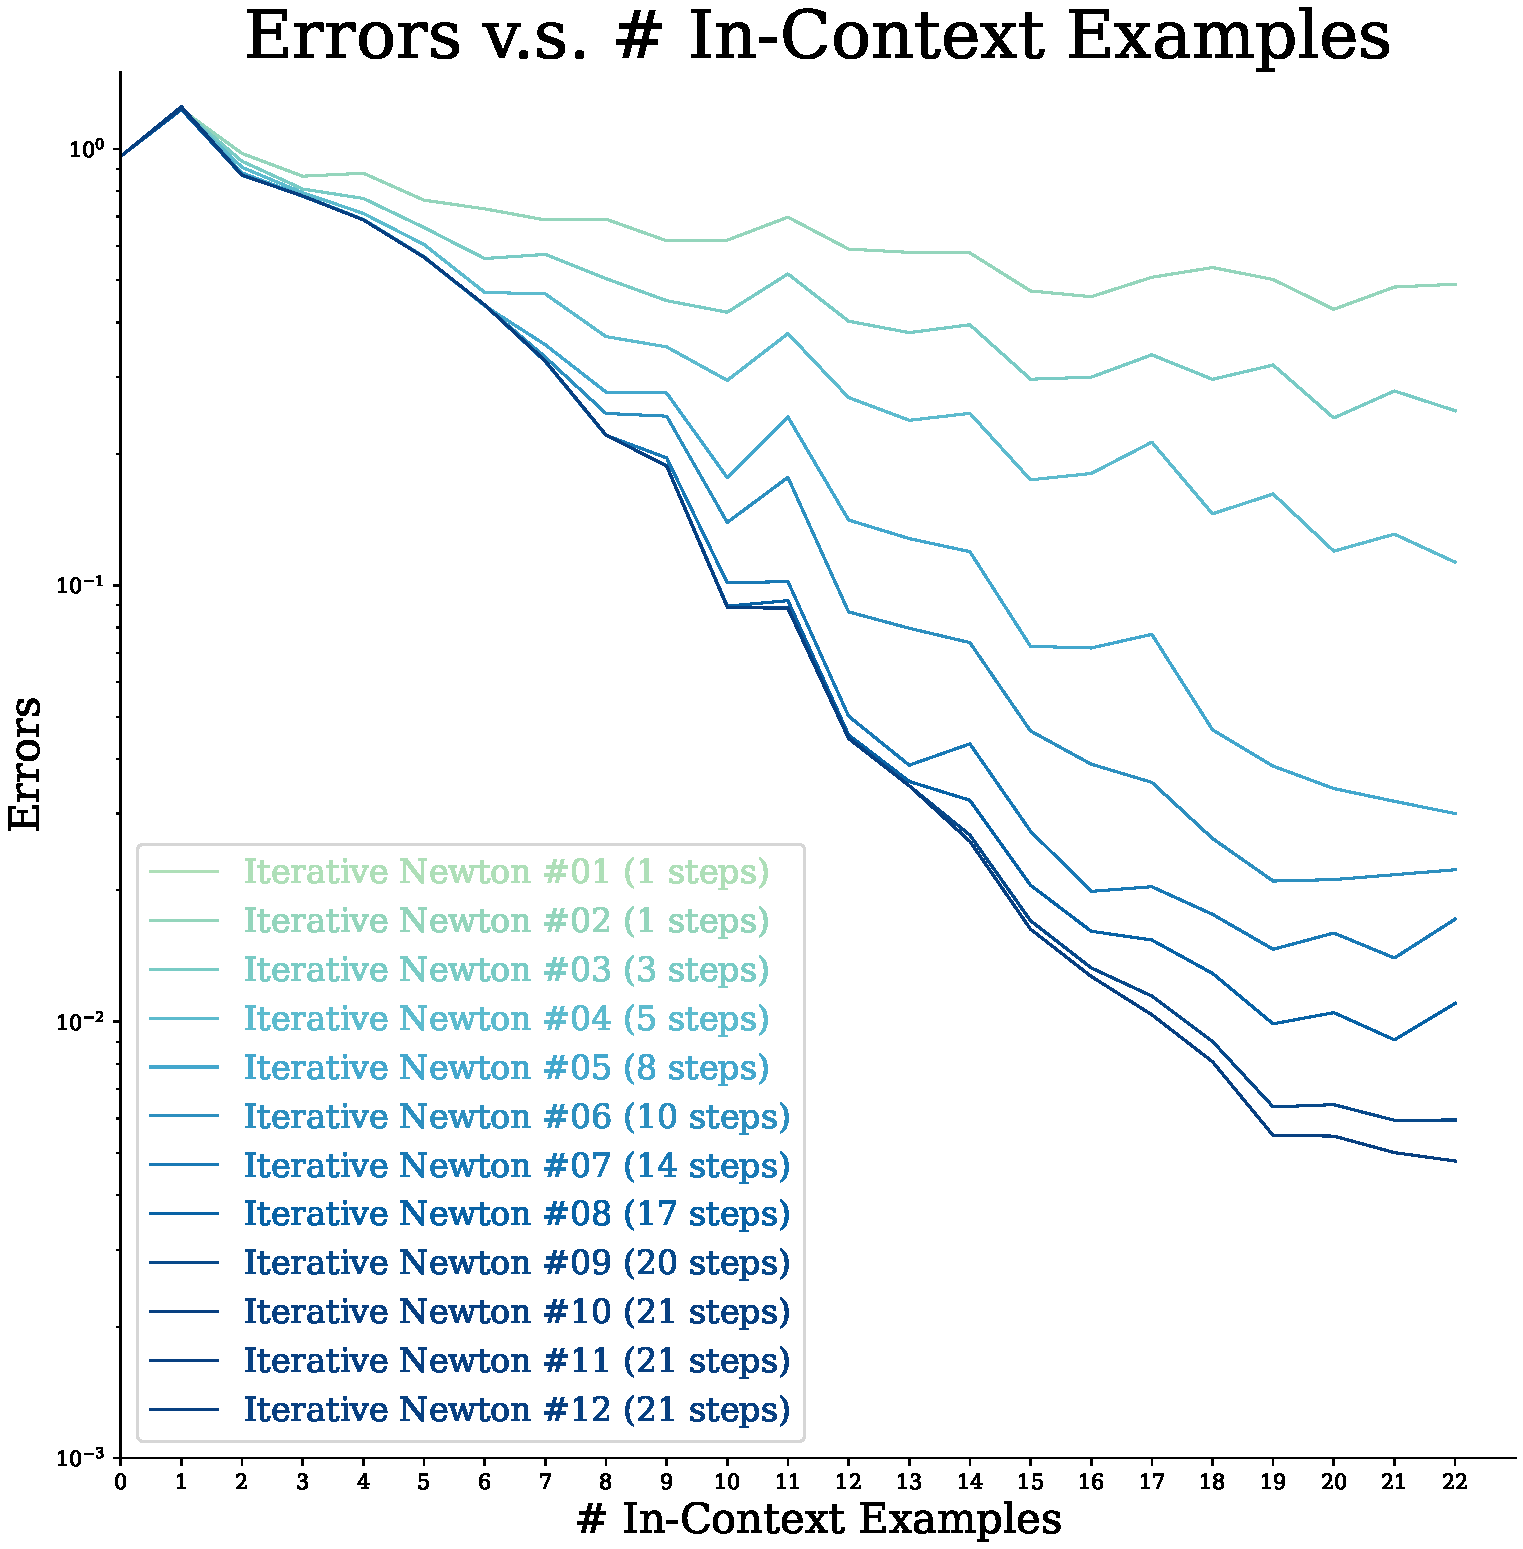
\includegraphics[width=0.4\linewidth]{Figures/progression/newton_skew_only.pdf}} \label{subfig:newton_skew_only}
    \caption{\textbf{Progression of Algorithms on Ill-Conditioned Data.} Transformer's performance still improves over the layer index $\ell$; Iterative Newton's Method's performance improves over the number of iterations $t$ and we plot the best-matching $t$ to Transformer's $\ell$ following \cref{def:matching}.}
    \label{fig:progression_skew}
\end{figure}

We also present the heatmaps to find the best-matching steps and conclude that Transformers are similar to Newton's method than GD in ill-conditioned data.
\begin{figure}[!htp]
    \centering

\includegraphics[width=0.49\linewidth]{Figures/ill/resid_sim_heatmap_tf_newton_full.pdf}

\includegraphics[width=0.49\linewidth]{Figures/ill/resid_sim_heatmap_tf_gd_full.pdf}
\caption{\textbf{Similarity of Errors on Ill-Conditioned Data.} The best matching steps are highlighted in yellow.} \label{fig:ill_full_heatmap_sim_e}
\end{figure}

\begin{figure}[!htp]
    \centering

\includegraphics[width=0.49\linewidth]{Figures/ill/w_sim_heatmap_tf_newton_full.pdf}

\includegraphics[width=0.49\linewidth]{Figures/ill/w_sim_heatmap_tf_gd_full.pdf}
\caption{\textbf{Similarity of Induced Weights on Ill-Conditioned Data.} The best matching steps are highlighted in yellow.} \label{fig:ill_full_heatmap_sim_w}
\end{figure}

\begin{figure}[!htp]
    \centering
\subfigure[Transformer v.s. BFGS]{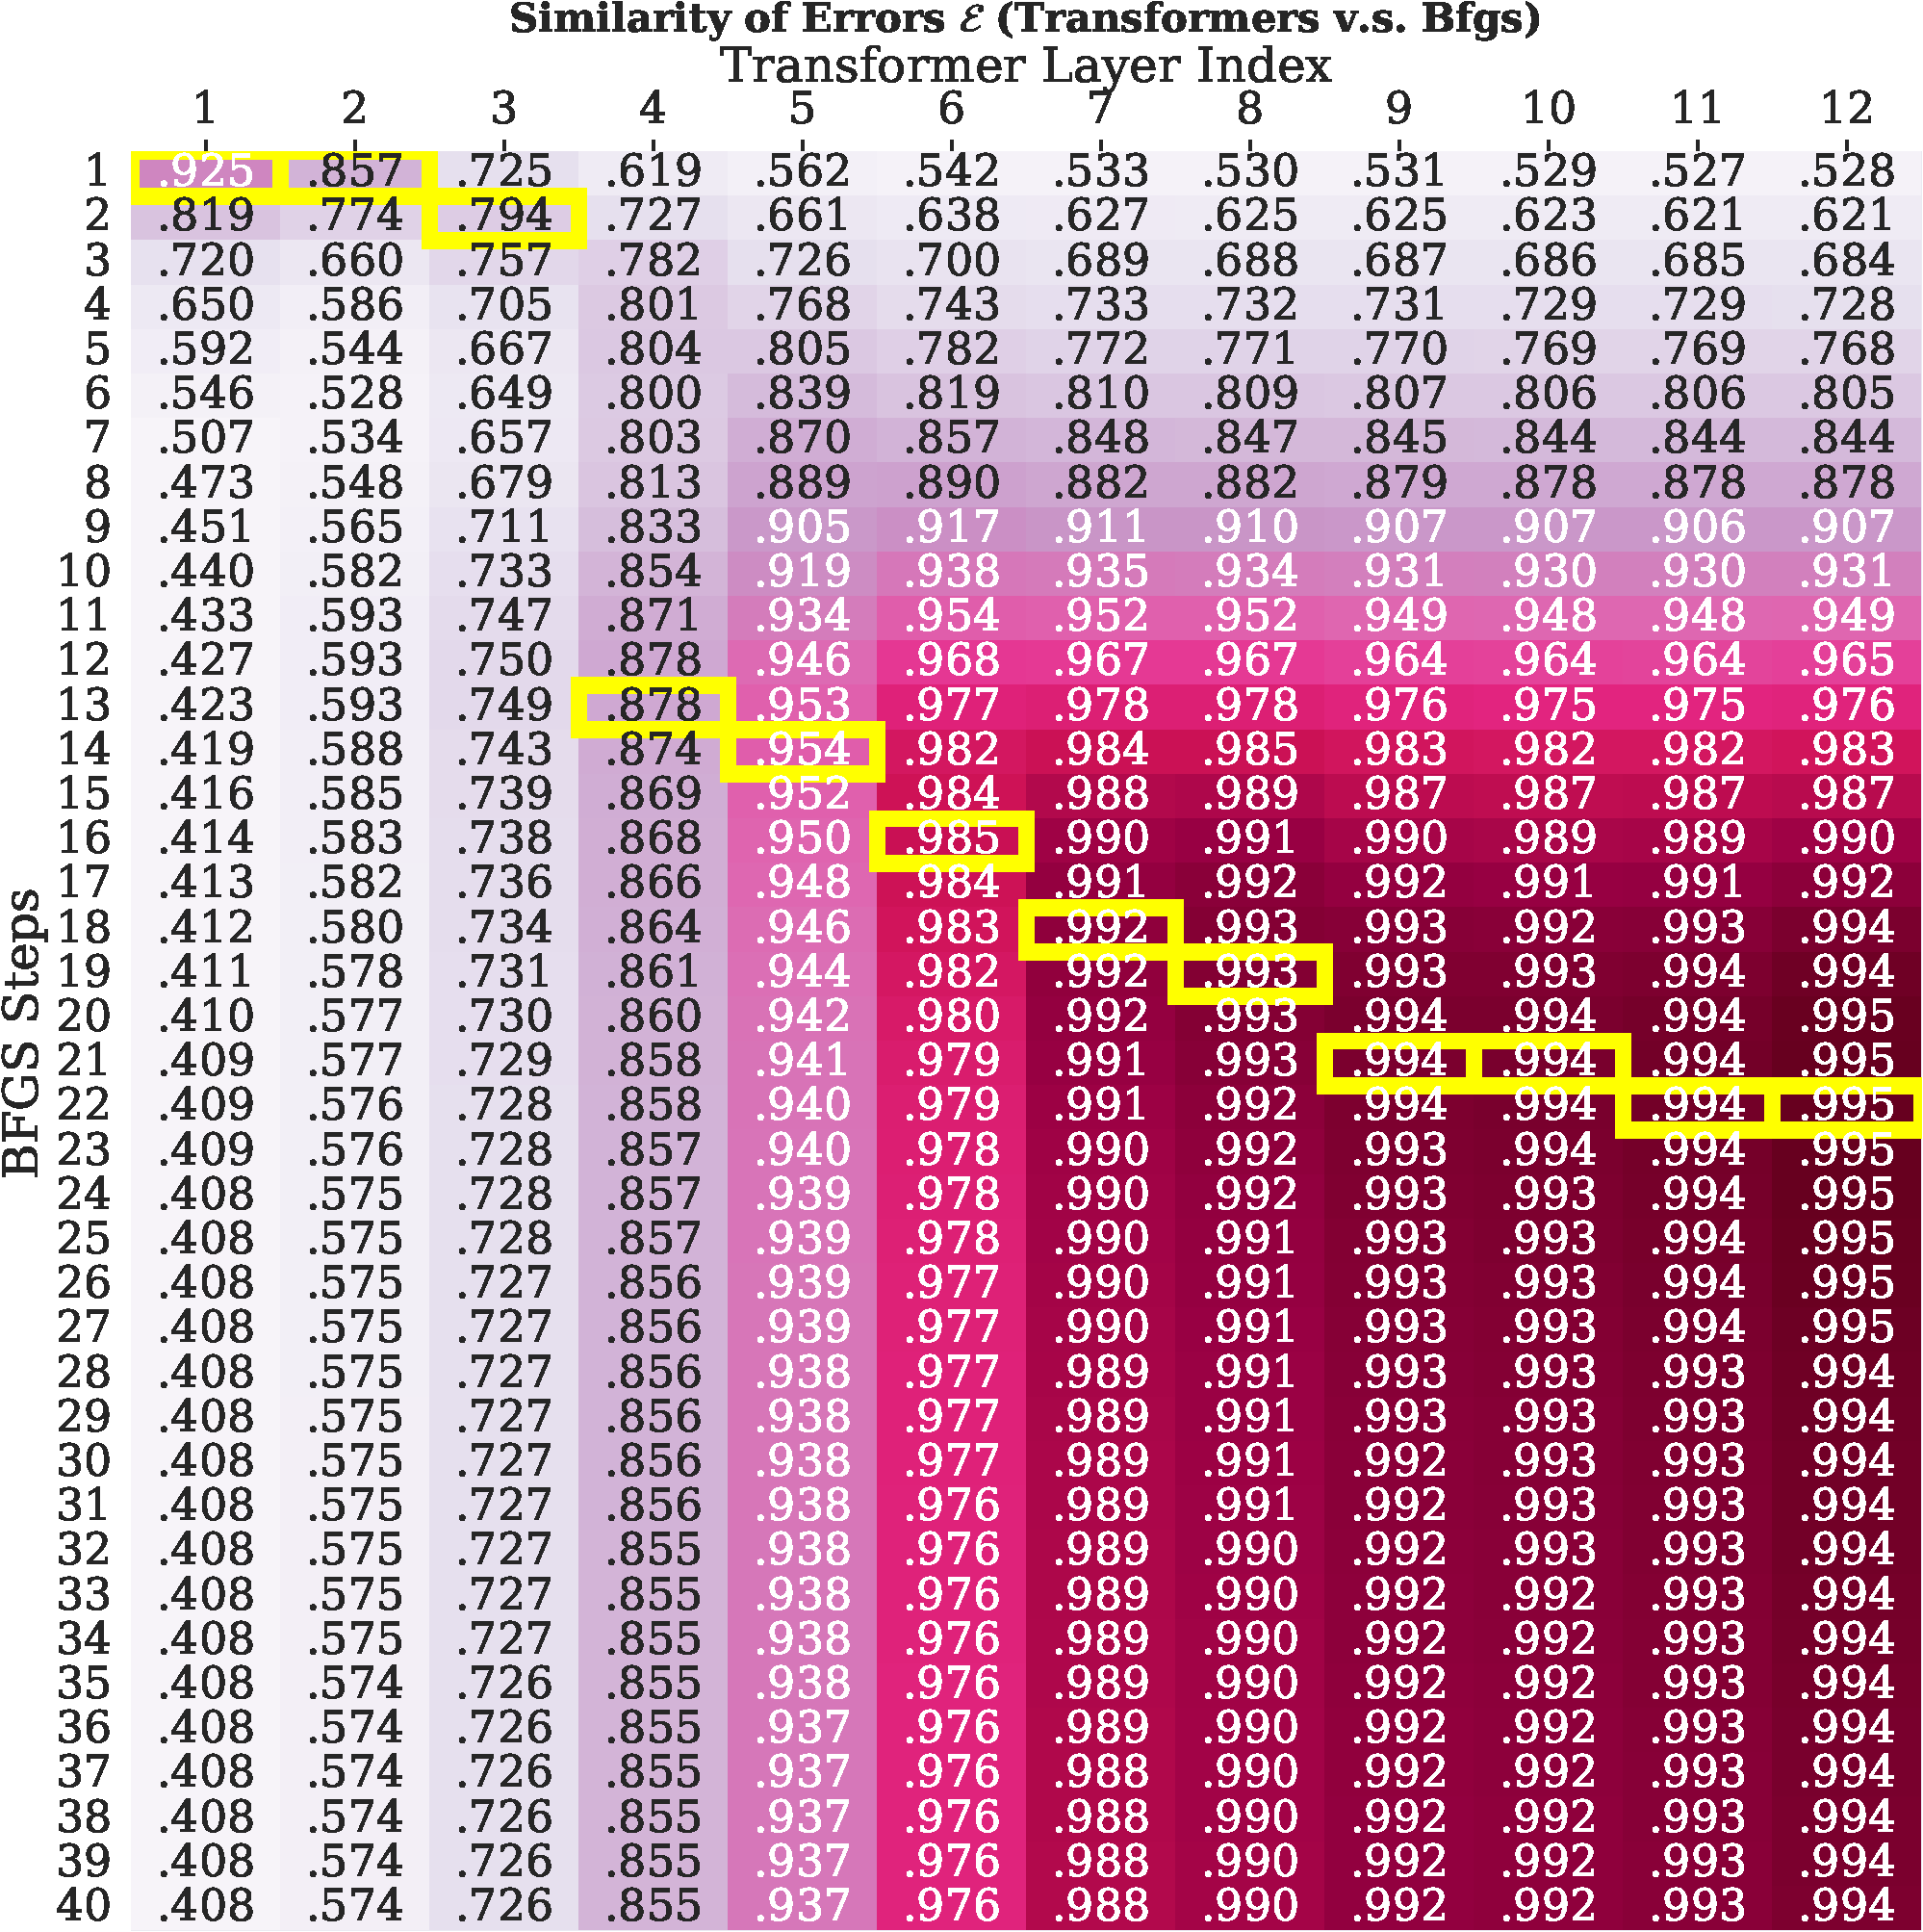
\includegraphics[width=0.49\linewidth]{Figures/ill/resid_sim_heatmap_tf_bfgs_full_ill.pdf}}
\subfigure[Transformer v.s. L-BFGS]{
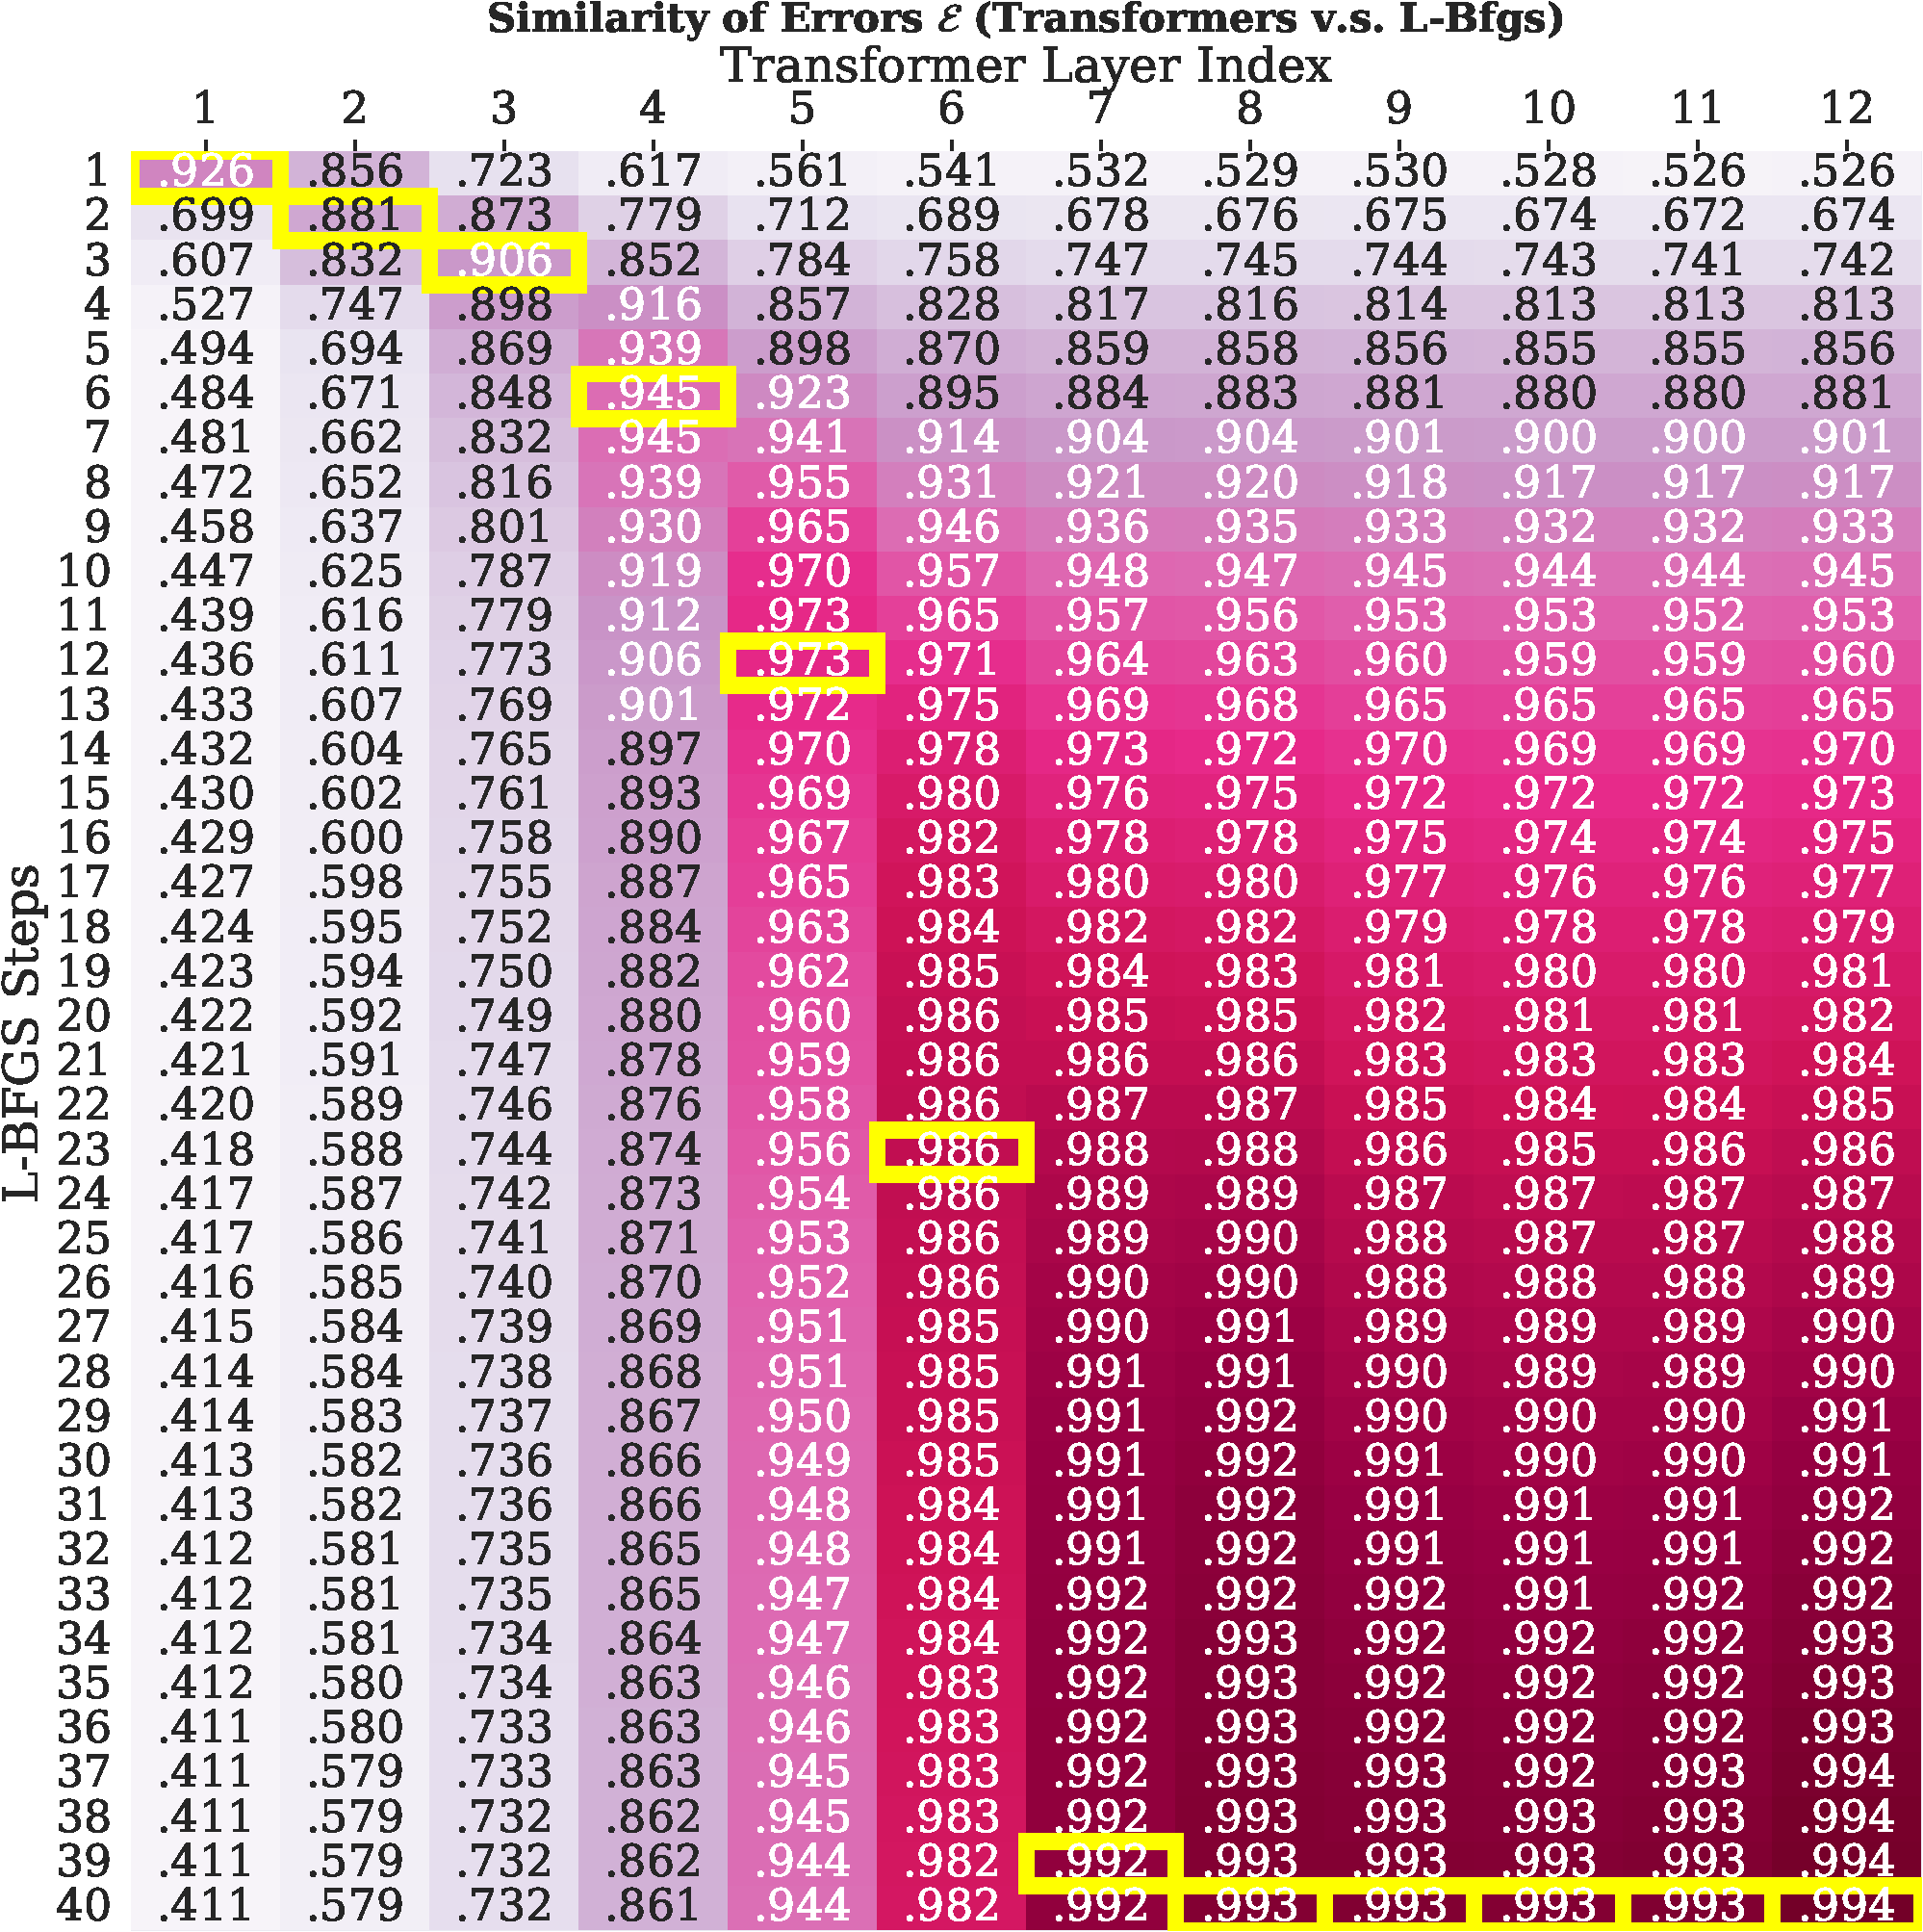
\includegraphics[width=0.49\linewidth]{Figures/ill/resid_sim_heatmap_tf_l-bfgs_full_ill.pdf}
}
\caption{\textbf{Similarity of Errors on Ill-Conditioned Data with Quasi-Newton Methods.} The best matching steps are highlighted in yellow. Transformer also matches BFGS linearly, from layers 4 to 11. L-BFGS still suffers due to its limited memory but still better than \gd because L-BFGS also attempts to approximate second-order information.} \label{fig:ill_bfgs}
\end{figure}

\clearpage
\subsubsection{Experiments with Noisy Linear Regression} \label{ssec:noisy}
We repeat the same experiments on noisy linear regression tasks with $y = \bw^\top \bx + \varepsilon$ where $\varepsilon \sim \mathcal N(0, \sigma^2)$ with noise level $\sigma = 0.1$. As shown in Figure \ref{fig:noisy-lr}, Transformers still show superlinear convergence on noisy linear regression tasks. Since the predictor is $\hat{\bw} = \left(\bX^\top \bX + \lambda \bI\right)^\dagger \bX^\top \by$ for some $\lambda$, the iterative newton's method is applied to $\bS = \bX^\top \bX + \lambda \bI$. Iterative Newton's method still keeps the same superlinear convergence rates. As it's also shown in Figure \ref{fig:noisy-lr}, Transformers and Iternative Newton's rates match linearly, as in the noiseless linear regression tasks. 
\begin{figure}[htp]
    \centering
      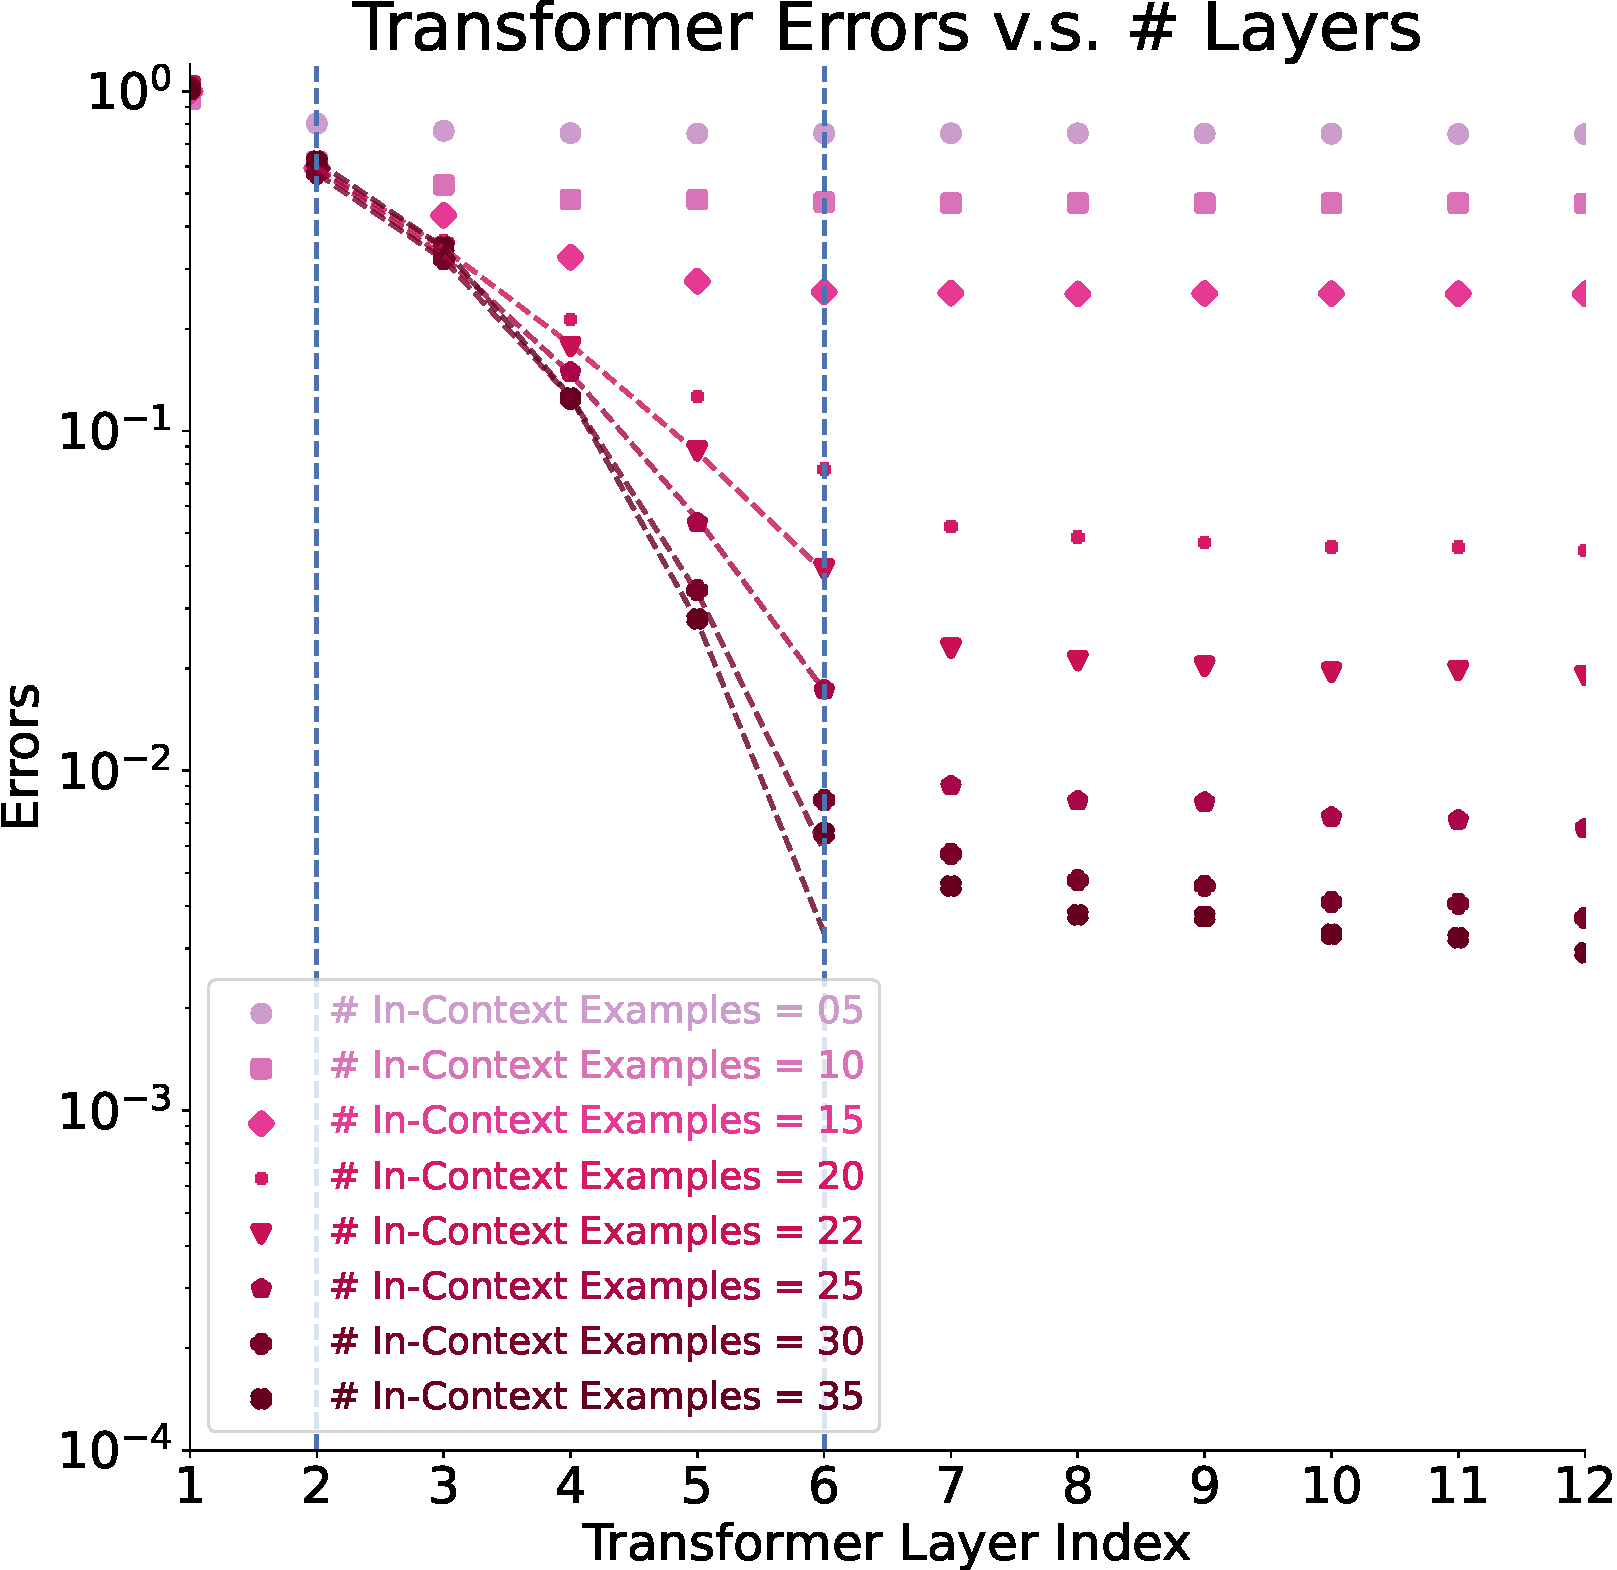
\includegraphics[width=0.45\linewidth]{Figures/noisy_lr/transformers_noisy_LR__error_new.pdf}
      
      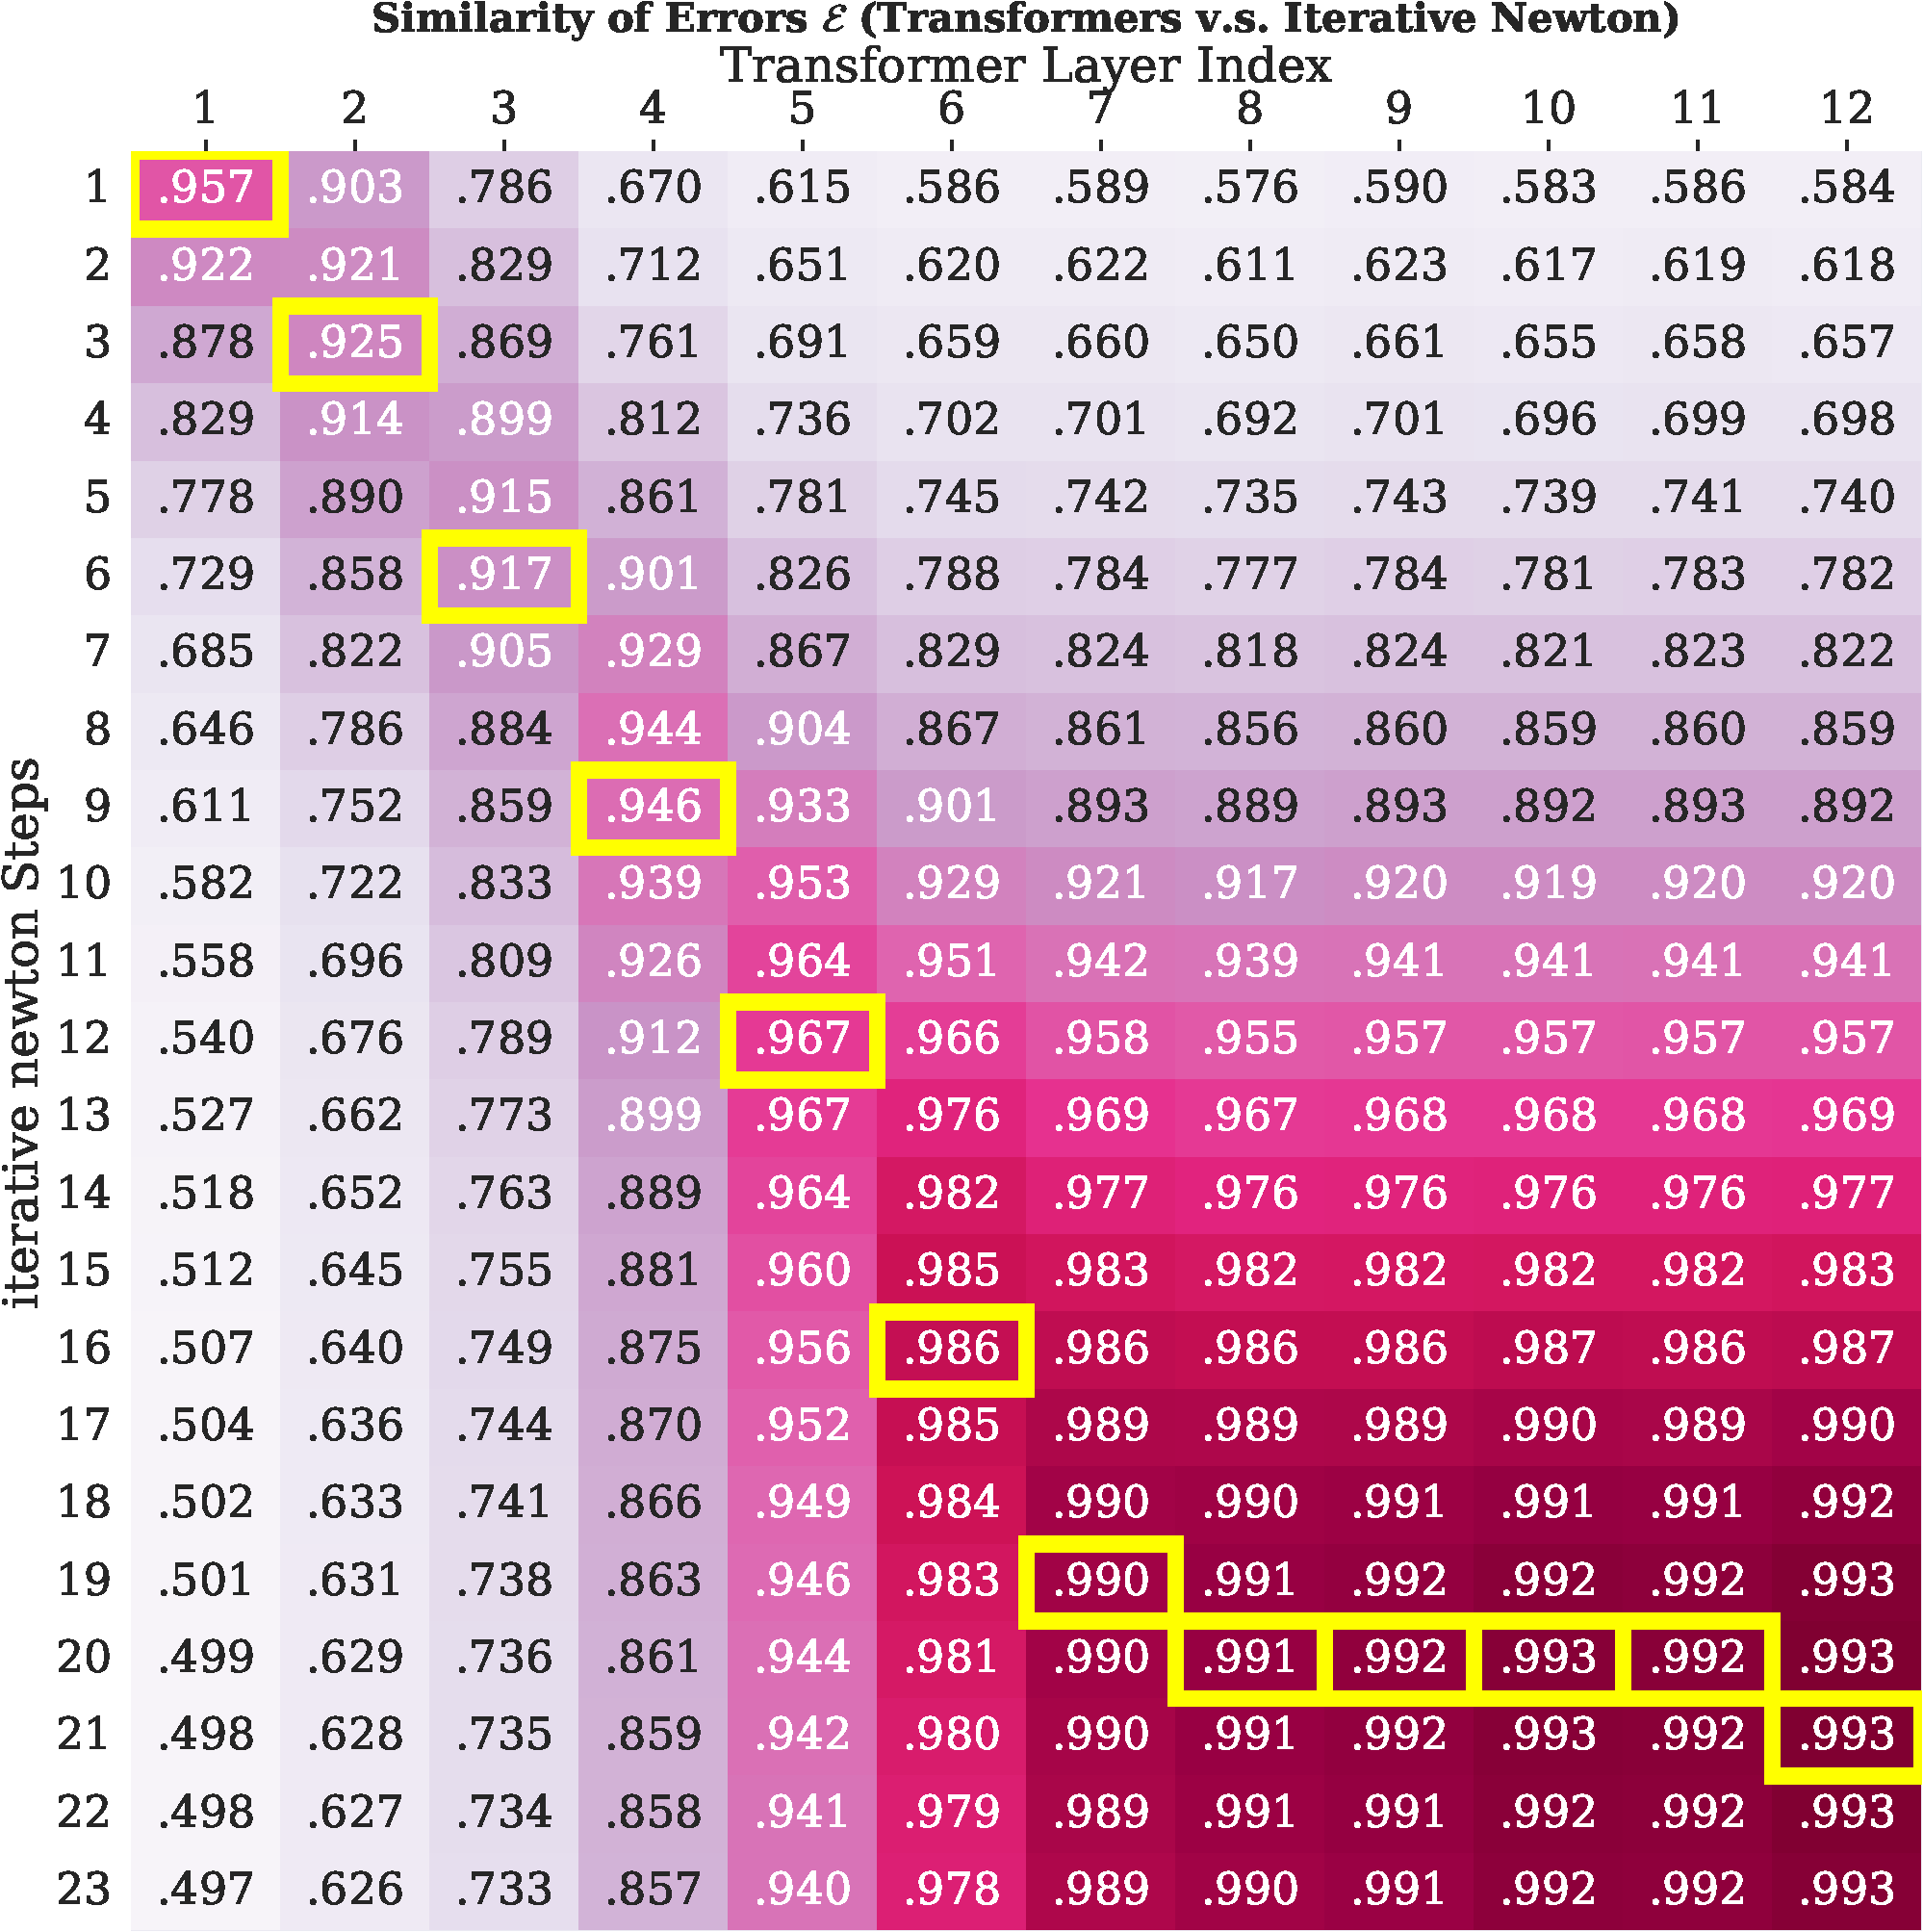
\includegraphics[width=0.45\linewidth]{Figures/noisy_lr/resid_sim_heatmap_tf_iterative_newton_full.pdf}
      \hfill
      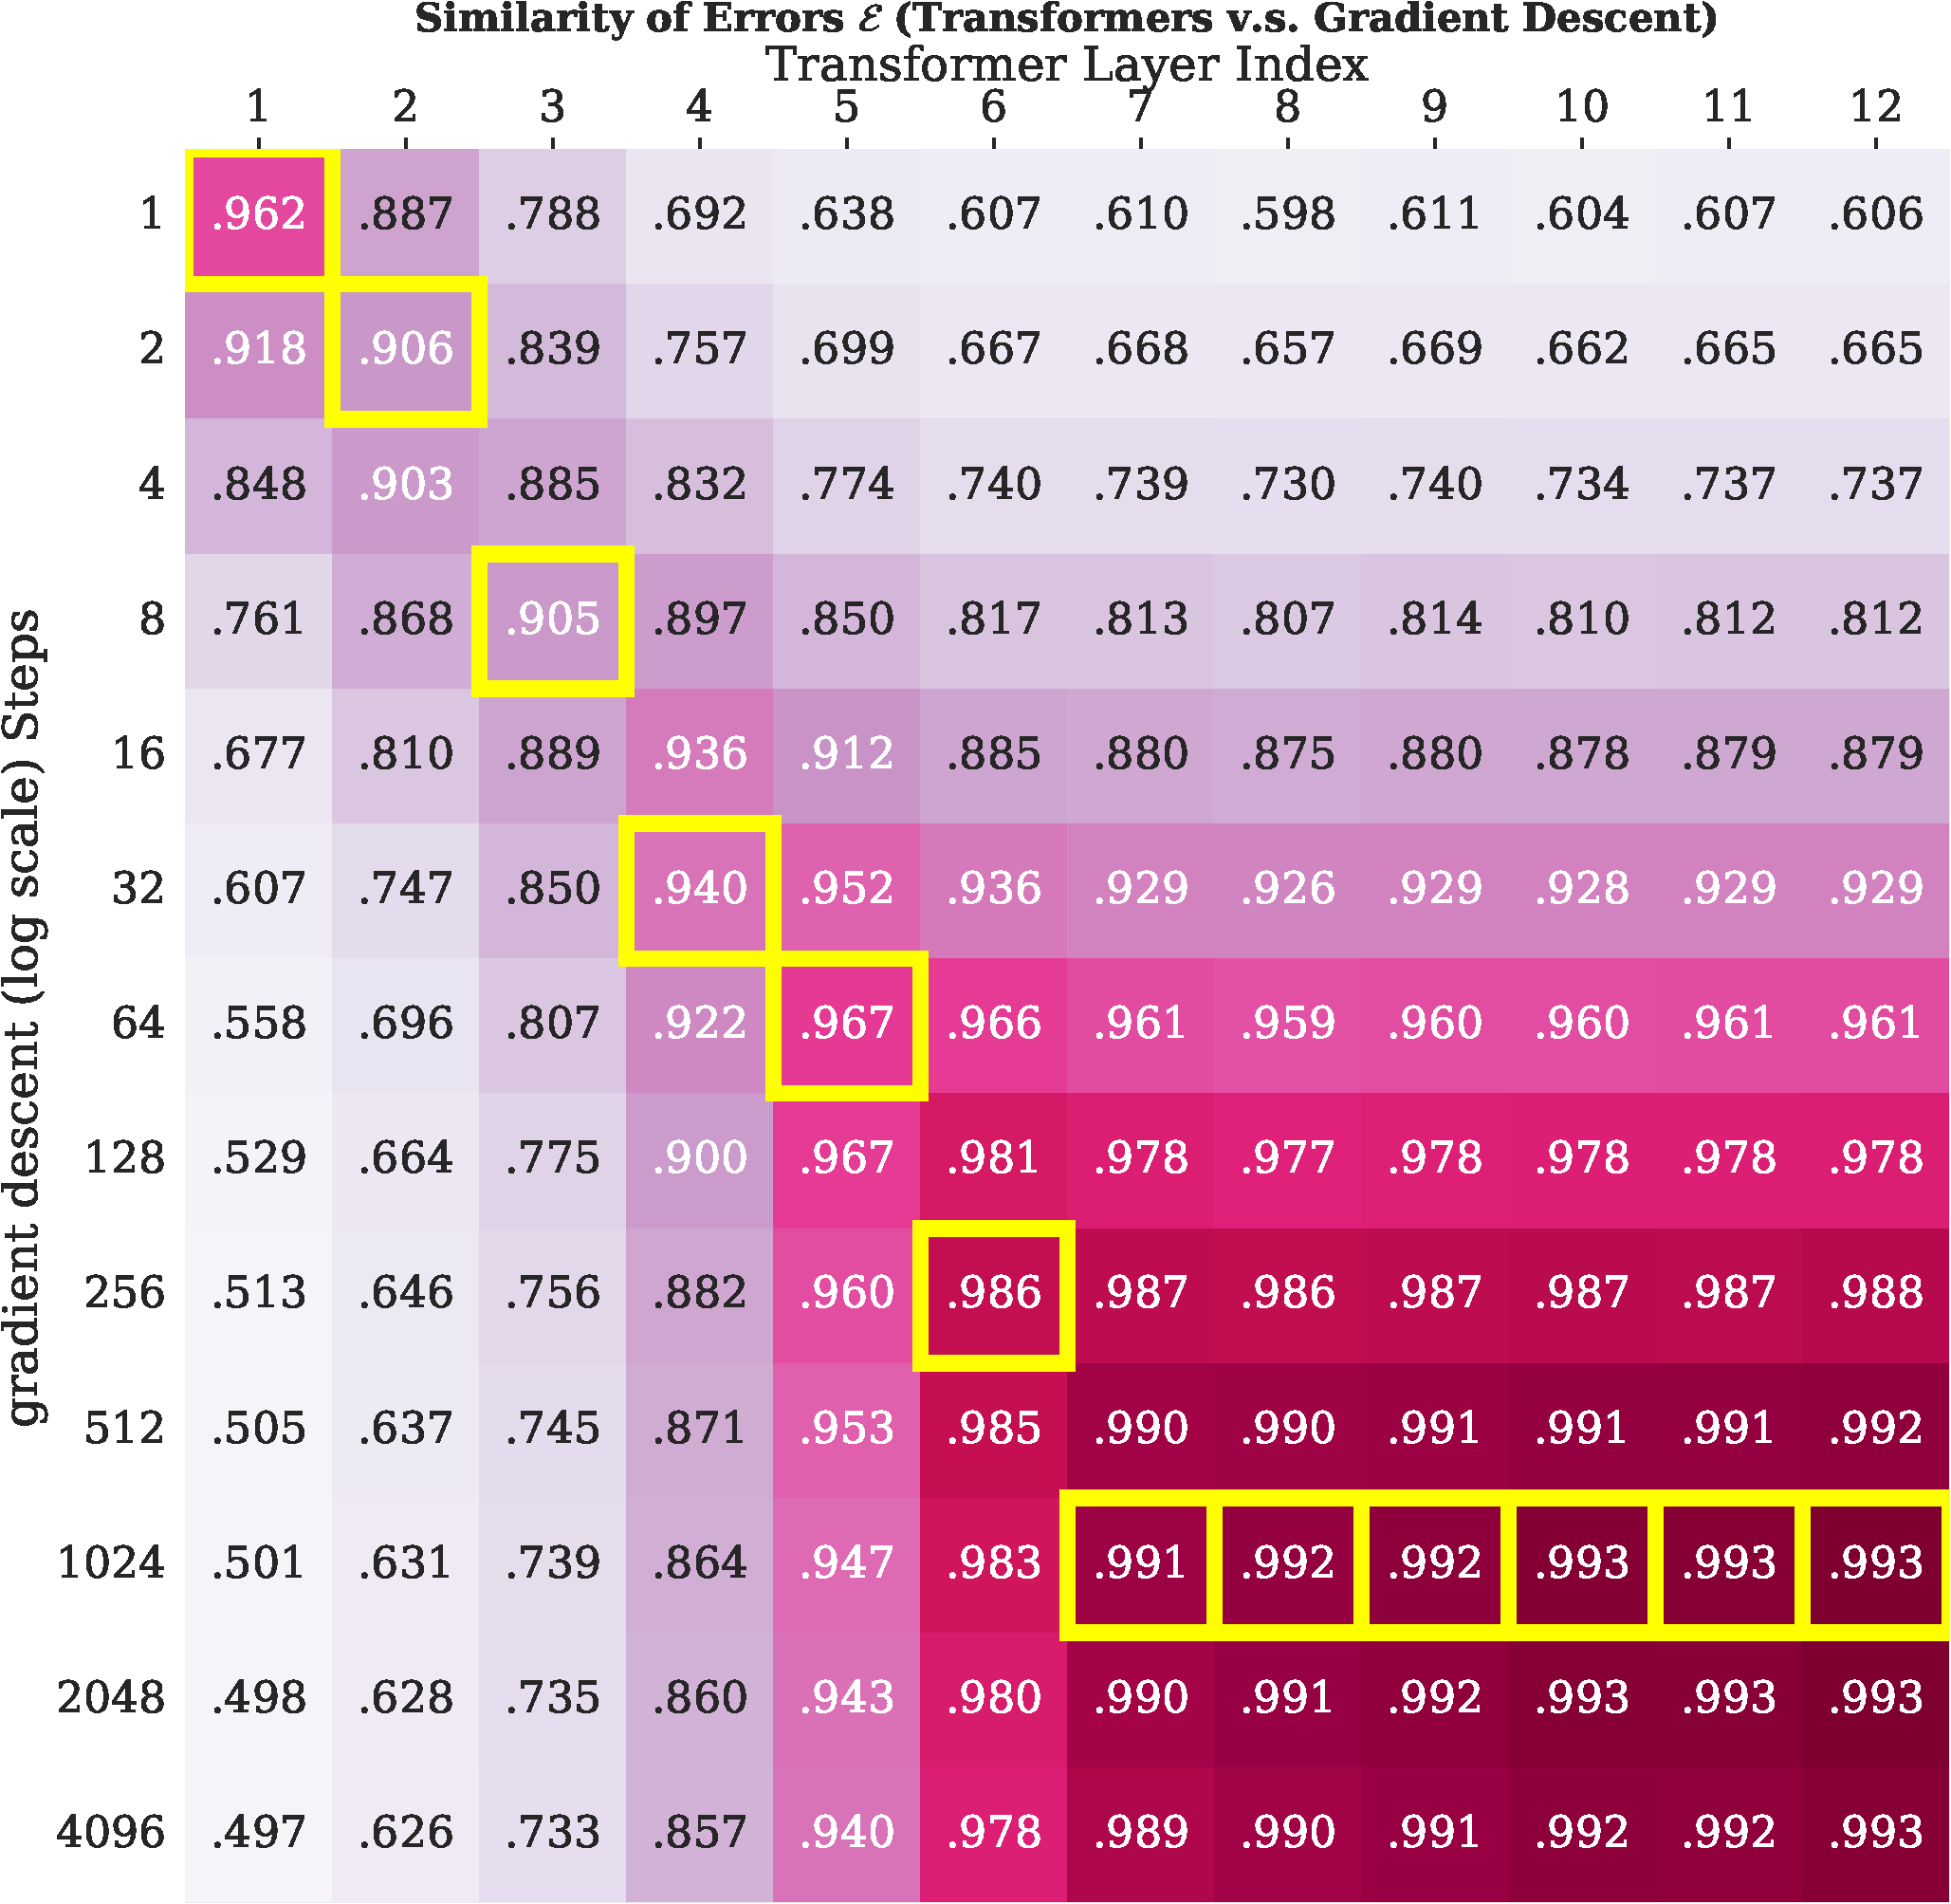
\includegraphics[width=0.45\linewidth]{Figures/noisy_lr/resid_sim_heatmap_tf_gradient_descent_log_scale_full.pdf}
      \caption{Experiment results on \textbf{Noisy Linear Regression}. \textbf{(Top)} Transformers have superlinear convergence rate. \textbf{(Bottom)} Transformers match Iterative Newton's rate and are exponentially faster than \gd.}
        \label{fig:noisy-lr}
\end{figure}

\subsubsection{Experiments with a Non-Linear Function Class (2-Layer MLP)} \label{app:non-linear}
To extend our experiments to non-linear cases, we adopt the same 2-layer ReLU neural network studied by \citet{Garg2022WhatCT}: see Fig. 5(c) in their paper. For any prompt $(\bx_1, y_1, \cdots, \bx_t, y_t)$, instead of generating labels $y_k = {\bw^\star}^\top \bx$ as mainly studied in the paper, we study a 2-layer neural network function class parameterized by $\bW \in \mathbb R^{d_\mathrm{hidden} \times d}$, $\bv \in \mathbb R^{d_\mathrm{hidden}}$, $\ba \in \mathbb R^{d_\mathrm{hidden}}$, and $b \in \mathbb R$, so that 
\begin{equation}
    y_k = f_{\bW, \bv, \ba, b}(\bx_k) = \ba^\top \mathrm{ReLU}\Big(\bW \bx_k + \bv\Big) + b
    \label{eqn:2nn-relu}
\end{equation}
Then we repeat the same probing experiments as in the main paper. As shown in Figure \ref{fig:transformer-relu2nn}, even on 2-layer neural network tasks with ReLU activation, Transformer shows superlinear convergence rates. Transformer shows an exponentially faster convergence rate than \gd's, because \gd's steps are shown in log scale and the trend is linear -- similar to Figure 9 in the main paper. 

\begin{figure}[htp]
    \centering
    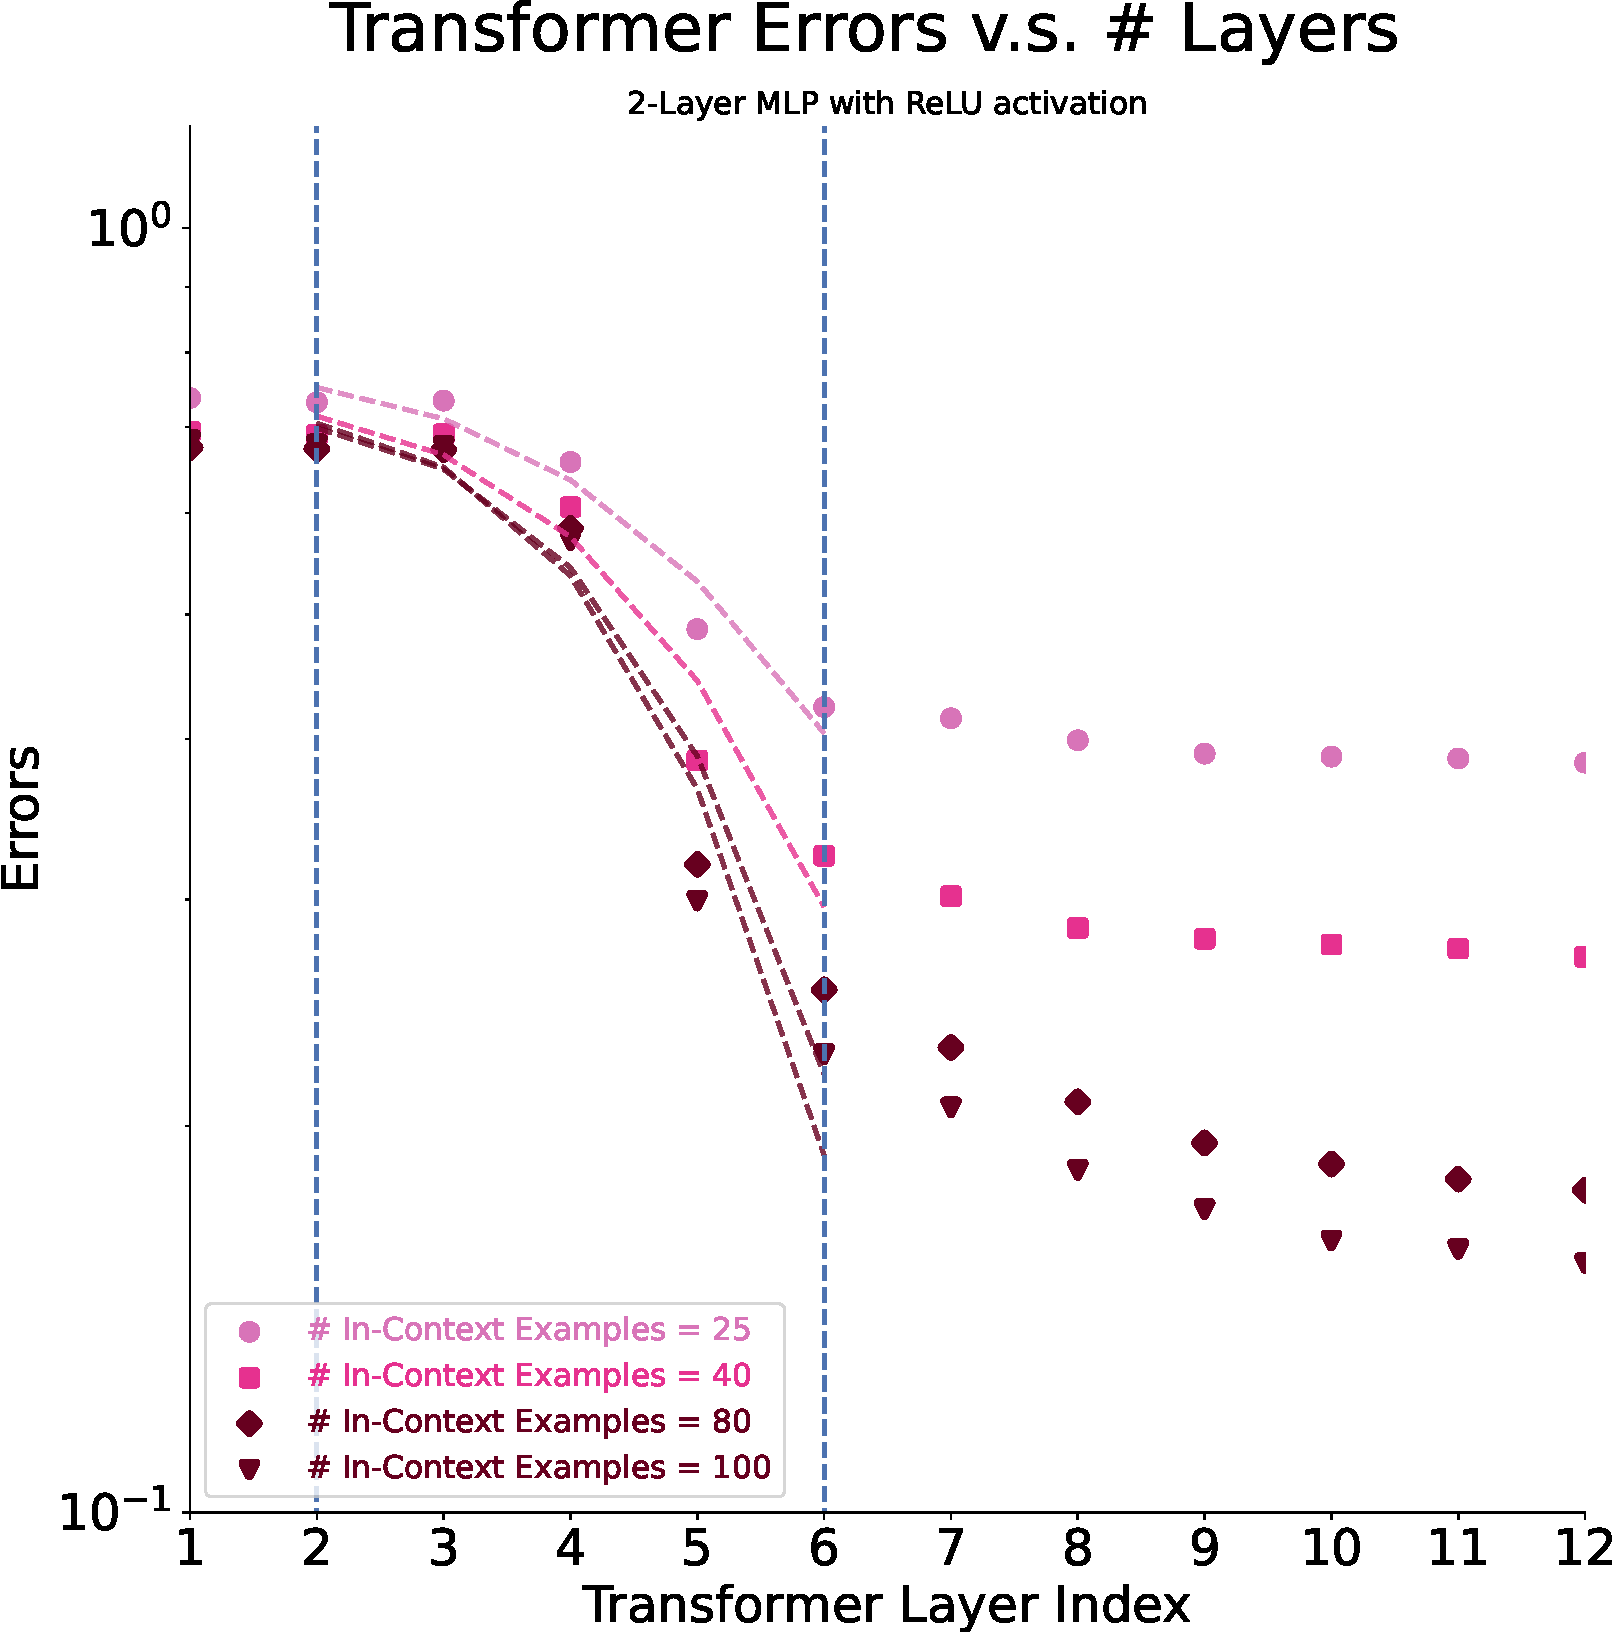
\includegraphics[width=0.49\linewidth]{Figures/nonlinear/transformers_RELU2NN__error.pdf}
    \hfill
  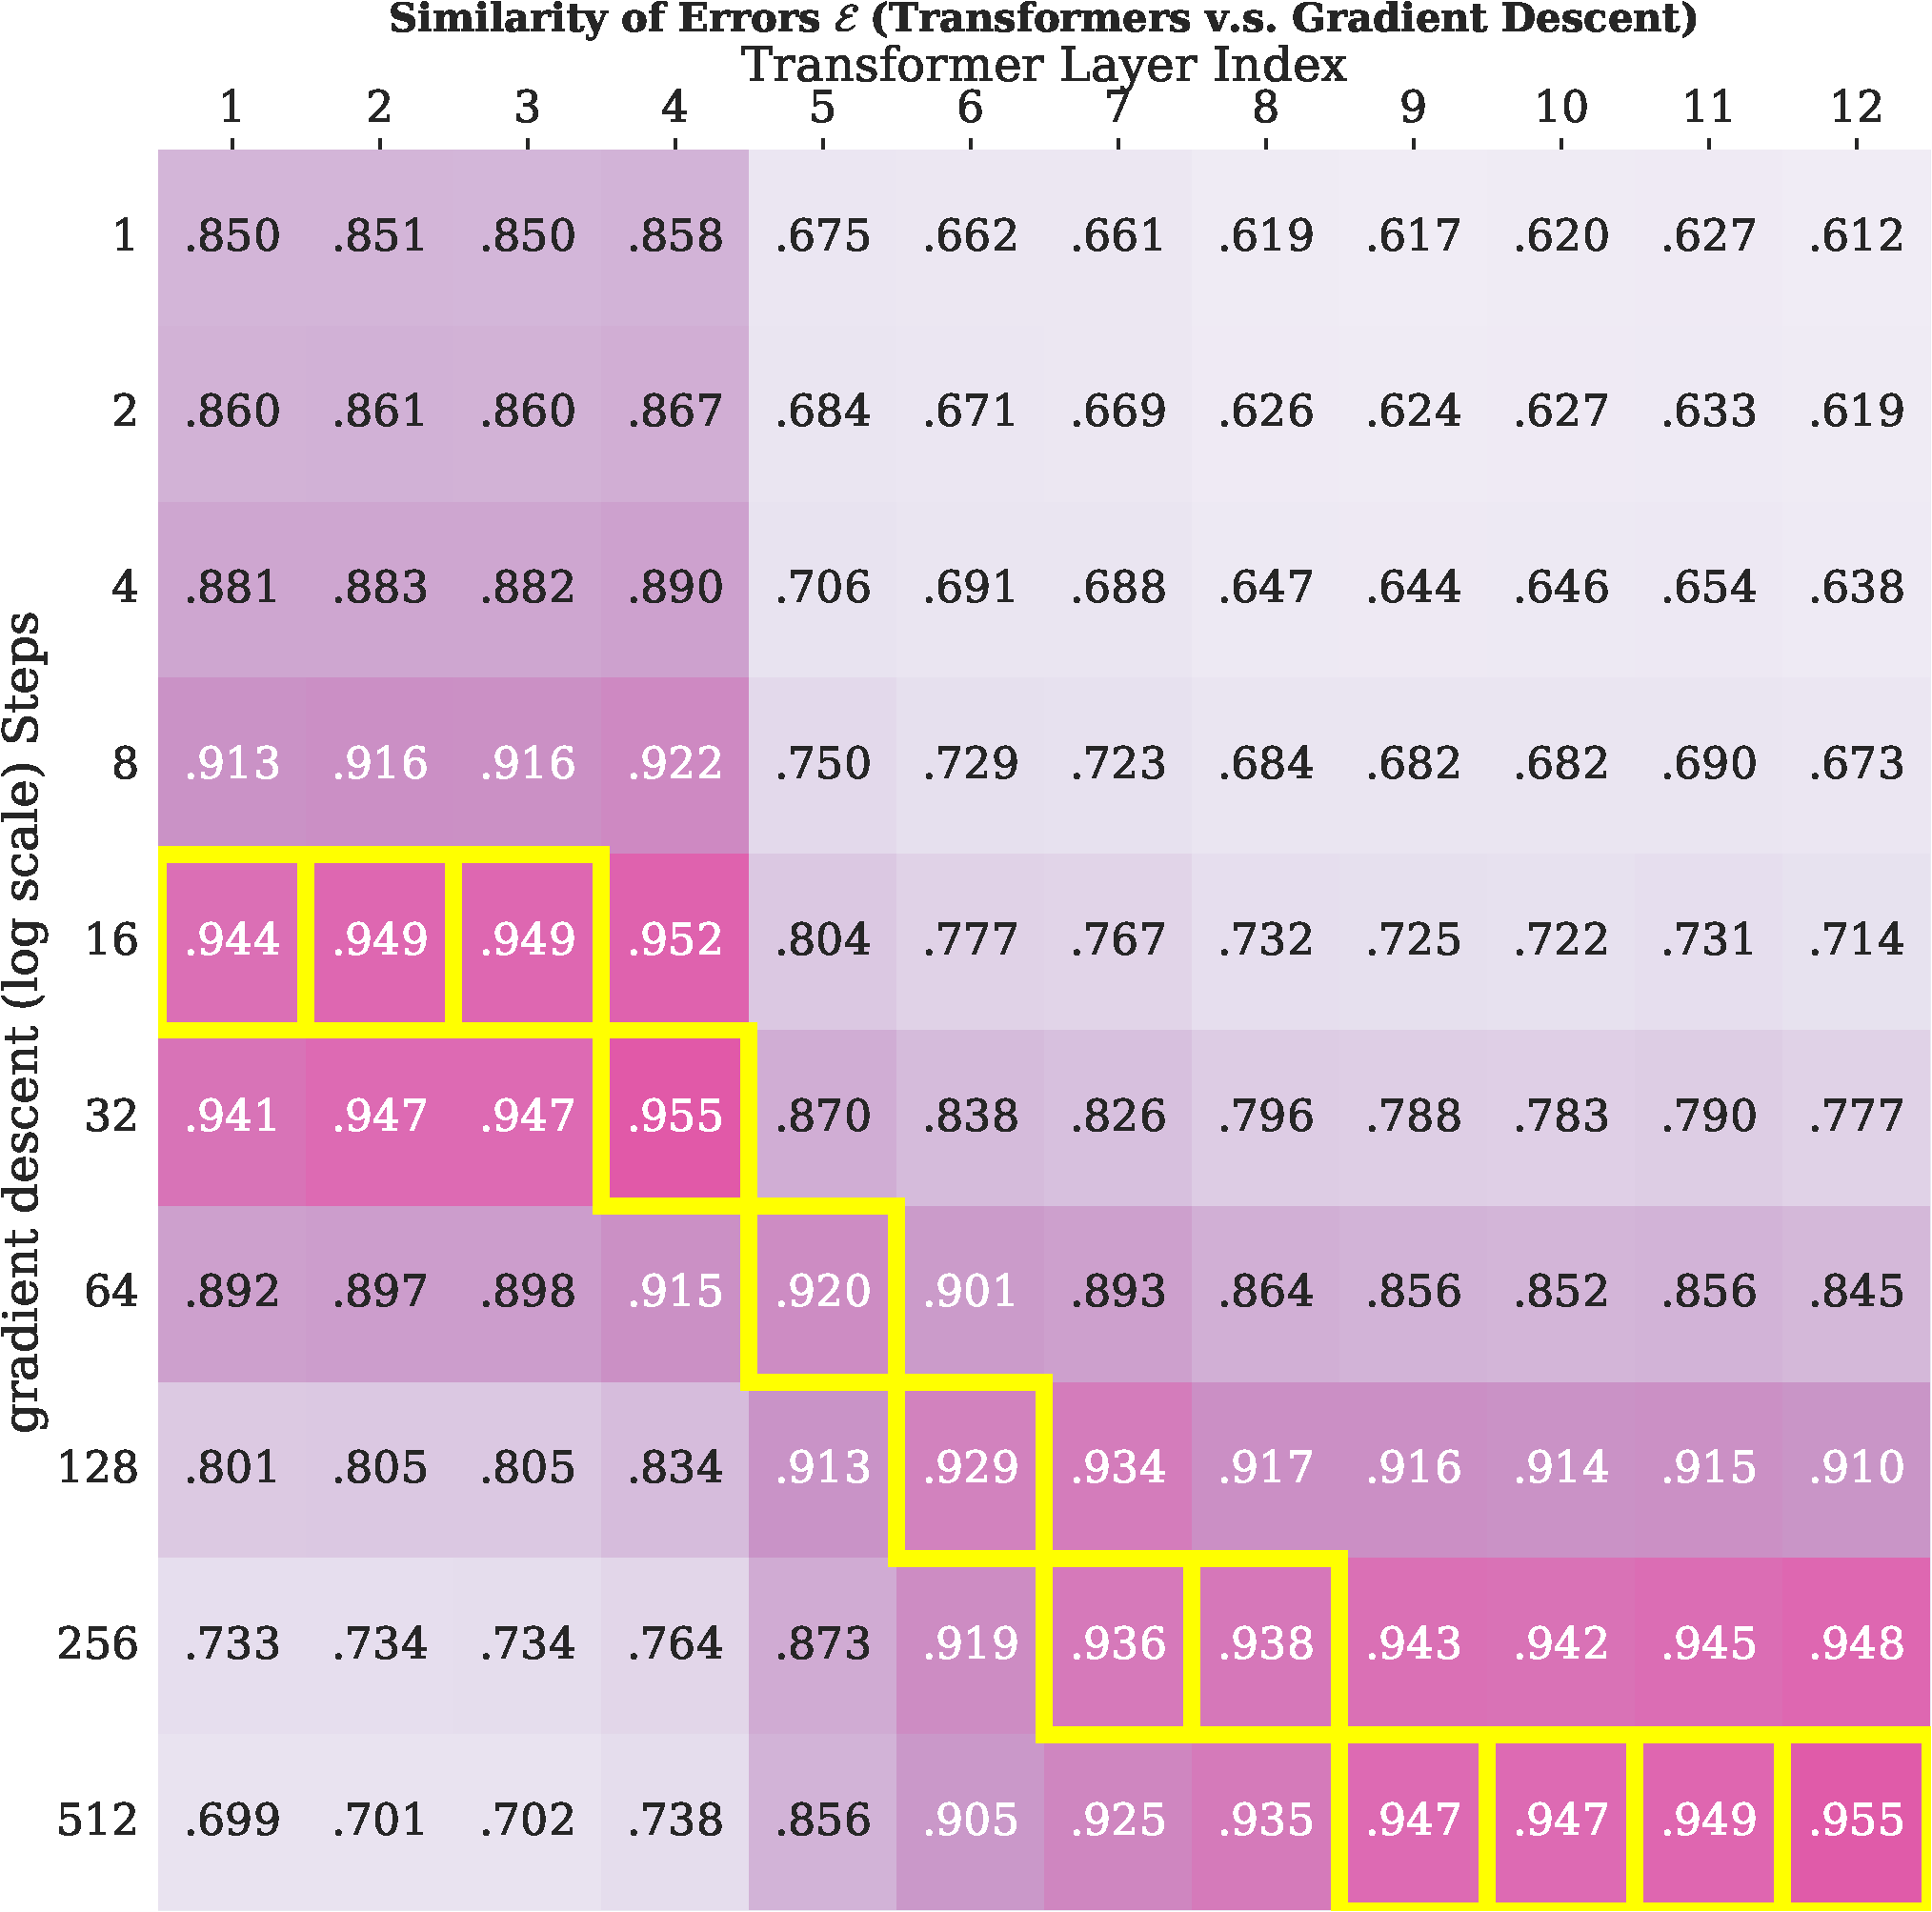
\includegraphics[width=0.49\linewidth]{Figures/nonlinear/resid_sim_heatmap_tf_gradient_descent_log_scale_relu2nn.pdf}
    \caption{Empirical Results on 2-Layer Neural Network Regression with ReLU activation function. Transformers have superlinear convergence rates and match \gd's convergence rate exponentially}
    \label{fig:transformer-relu2nn}
\end{figure}

It would be interesting to ablate the activation function used in \Cref{eqn:2nn-relu}. We further consider the case when it's using the Tanh activation instead of ReLU, i.e.

\begin{equation}
    y_k = f_{\bW, \bv, \ba, b}(\bx_k) = \ba^\top \mathrm{Tanh}\Big(\bW \bx_k + \bv\Big) + b
    \label{eqn:2nn-tanh}
\end{equation}

Repeating the same experiments as before, as shown in \Cref{fig:transformer-tanh2nn}, we find that Transformers use the entire first 5 layers to pre-process and then only in the next few layers show exponentially faster convergence rate compared to \gd. We further note that in both \Cref{fig:transformer-relu2nn} and \Cref{fig:transformer-tanh2nn}, the cosine similarities between Transformers and \gd\ are significantly lower than the experiments with linear regression tasks. This might due to the over-parameterization of the function class and Transformers and \gd\ may arrive at different optima. 

\begin{figure}[htp]
    \centering
    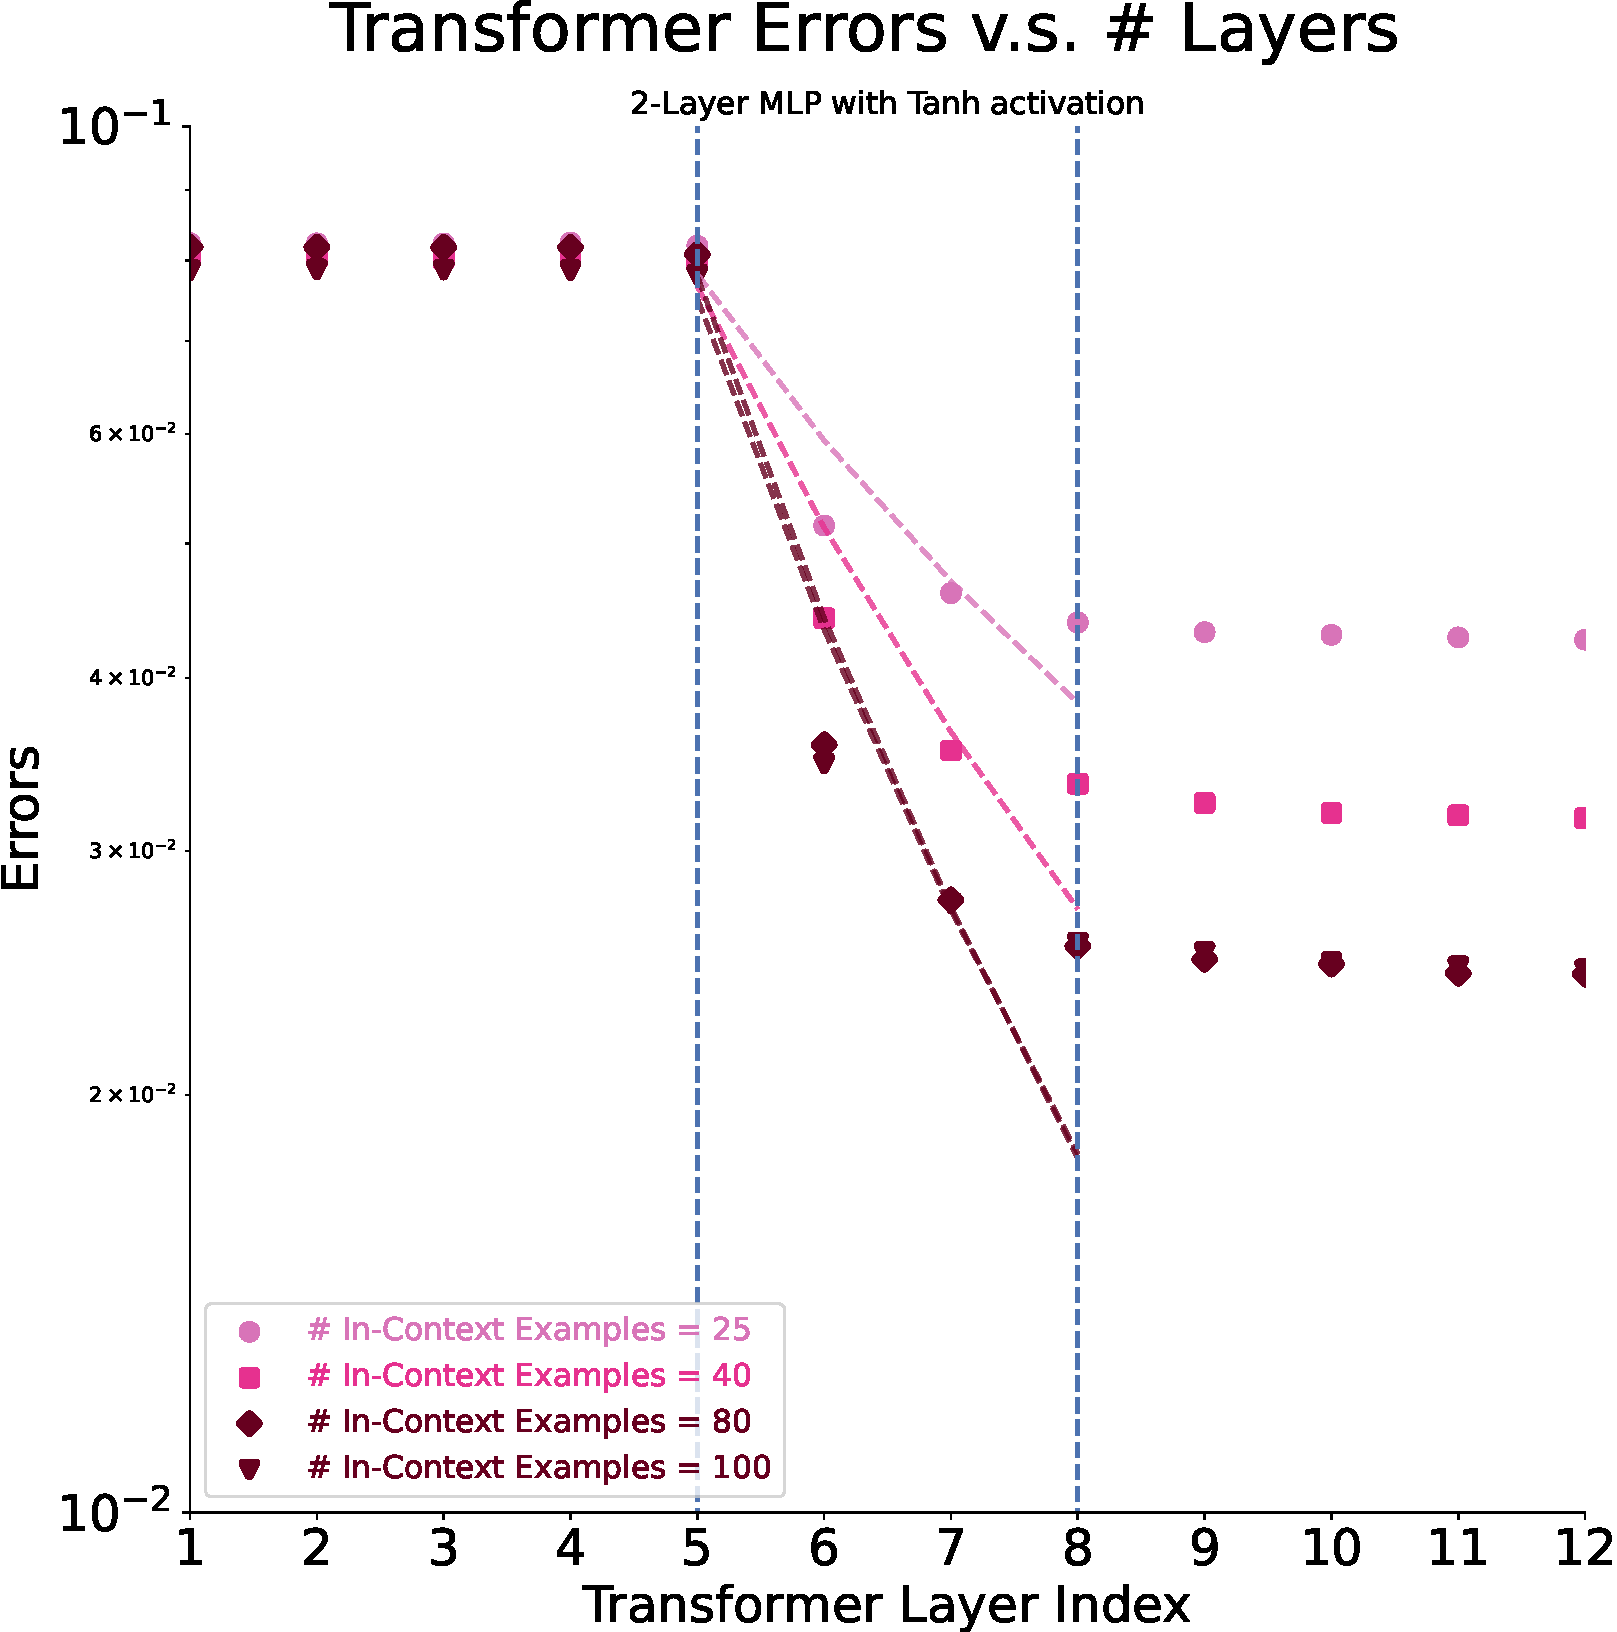
\includegraphics[width=0.49\linewidth]{Figures/nonlinear/transformers_Tanh2NN__error.pdf}
    \hfill
  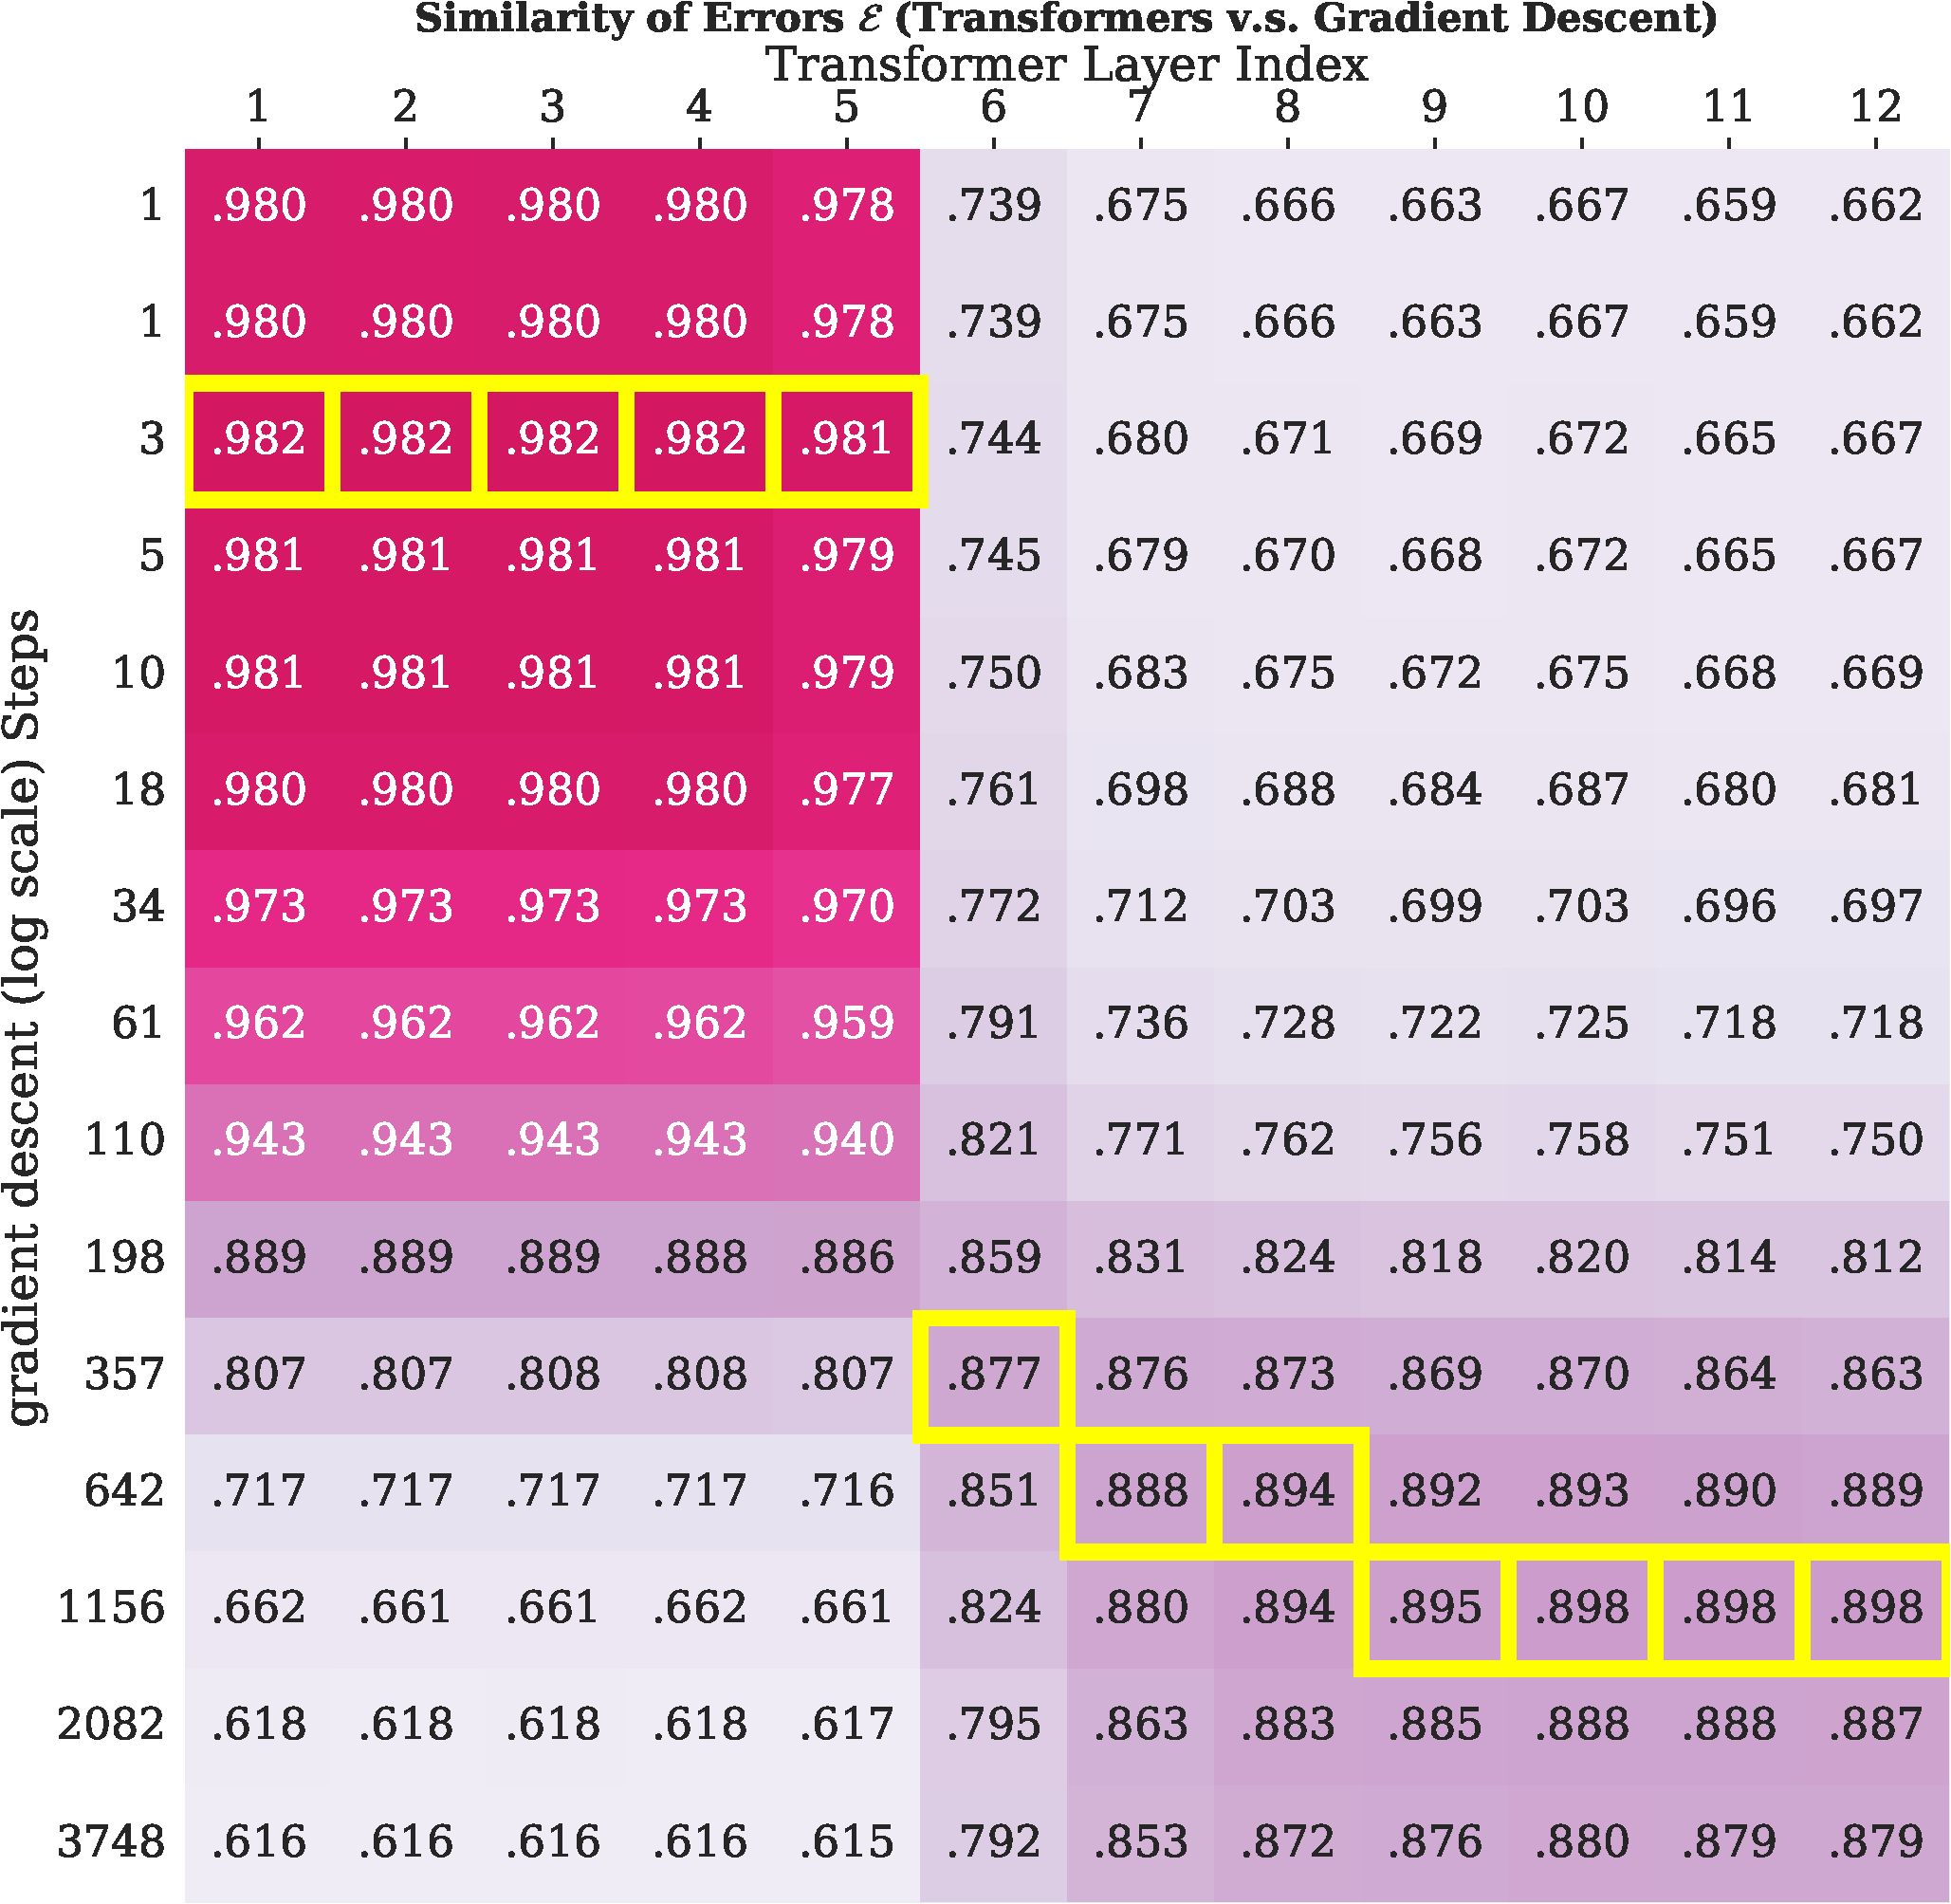
\includegraphics[width=0.49\linewidth]{Figures/nonlinear/resid_sim_heatmap_tf_gradient_descent_log_scale_tanh2nn.pdf}
    \caption{Empirical Results on 2-Layer Neural Network Regression with Tanh activation function. Transformers have superlinear convergence rates and match \gd's convergence rate exponentially}
    \label{fig:transformer-tanh2nn}
\end{figure}

It would be interesting for future research to explore further this function class of 2-layer MLP to understand fully how Transformer solve the regression problem in-context and whether it achieves a different optimum compared to alternative algorithms such as (Stochastic) \gd.
\clearpage
\subsection{Varying Transformer Architecture}
\subsubsection{Experiments on Transformers of Fewer Heads} \label{app:1-head}
In this section, we present experimental results from an alternative model configurations than the main text. We show in the main text that Transformers learn second-order optimization methods in-context where the experiments are using a GPT-2 model with 12 layers and 8 heads per layer. In this section, we present experiments with a GPT-2 model with 12 layers but only 1 head per layer. 

\begin{figure}[!htp]
    \centering
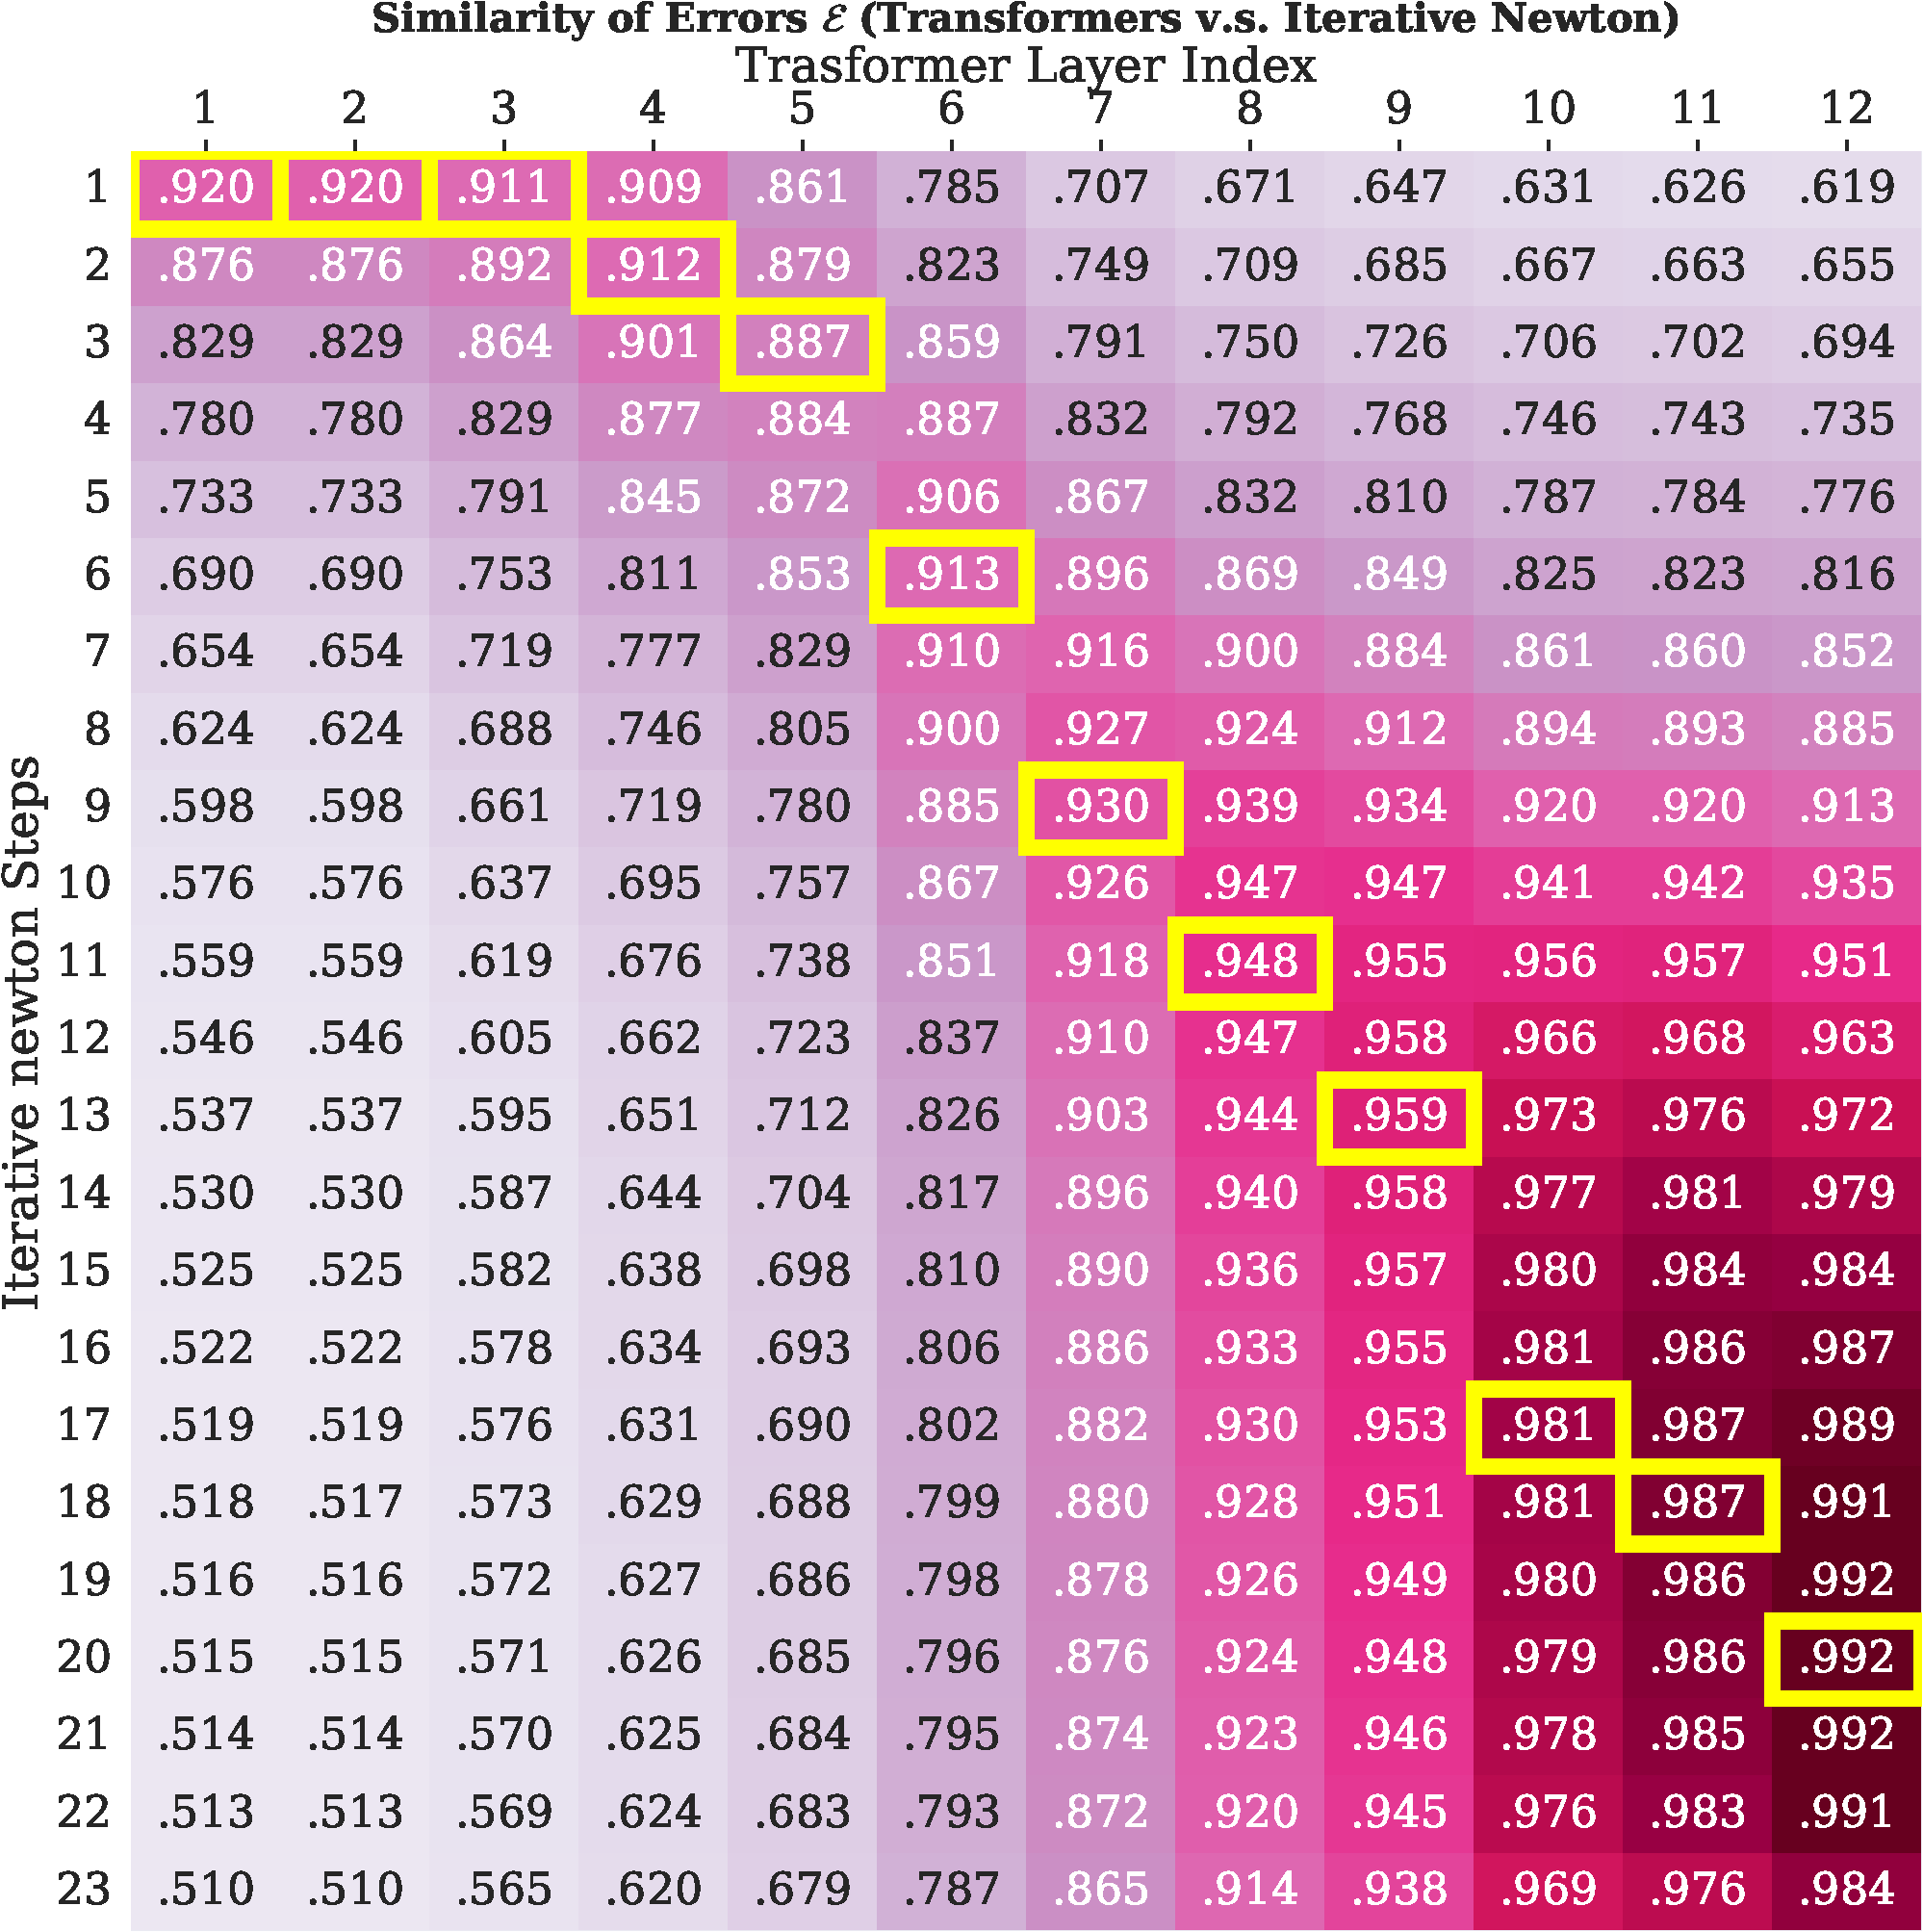
\includegraphics[width=0.45\linewidth]{Figures/12layer_1head/resid_sim_heatmap_tf_newton_full.pdf}
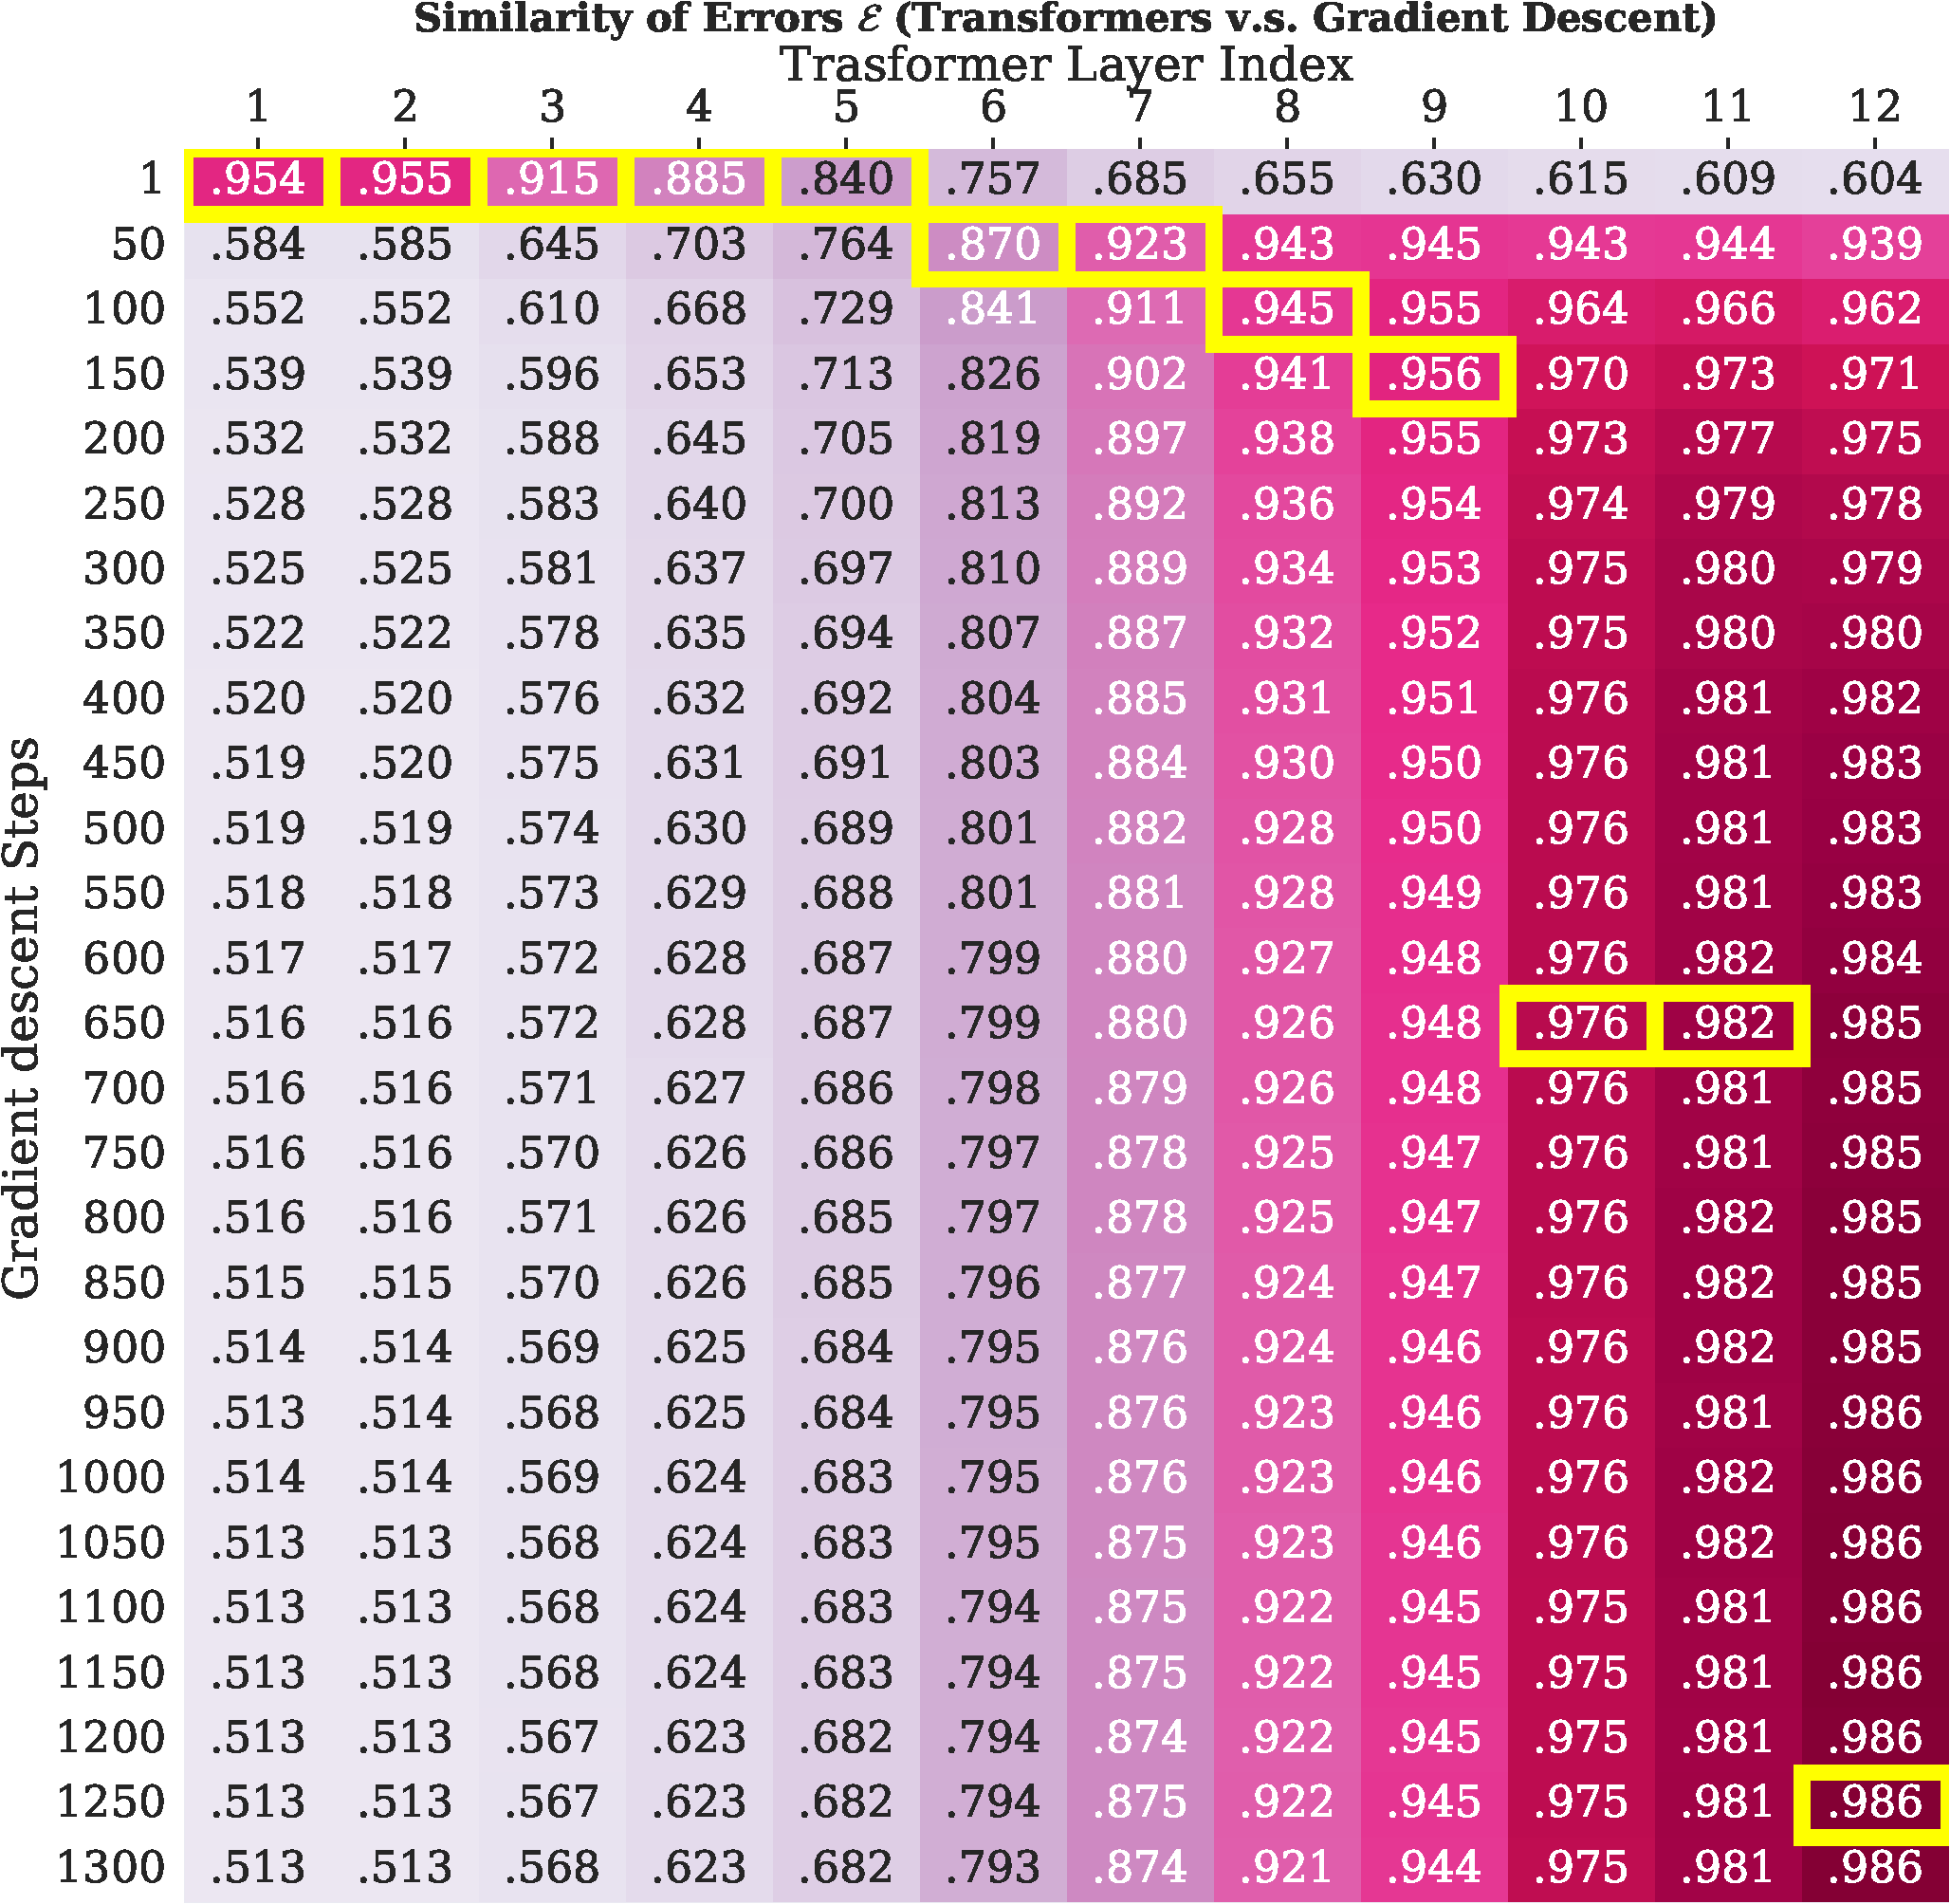
\includegraphics[width=0.45\linewidth]{Figures/12layer_1head/resid_sim_heatmap_tf_gd_full.pdf}
\caption{\textbf{Similarity of Errors on an alternative Transformers Configuration.} The best matching steps are highlighted in yellow. } \label{fig:12layer_1head_full_heatmap_sim_e}
\end{figure}
\begin{figure}[!htp]
    \centering
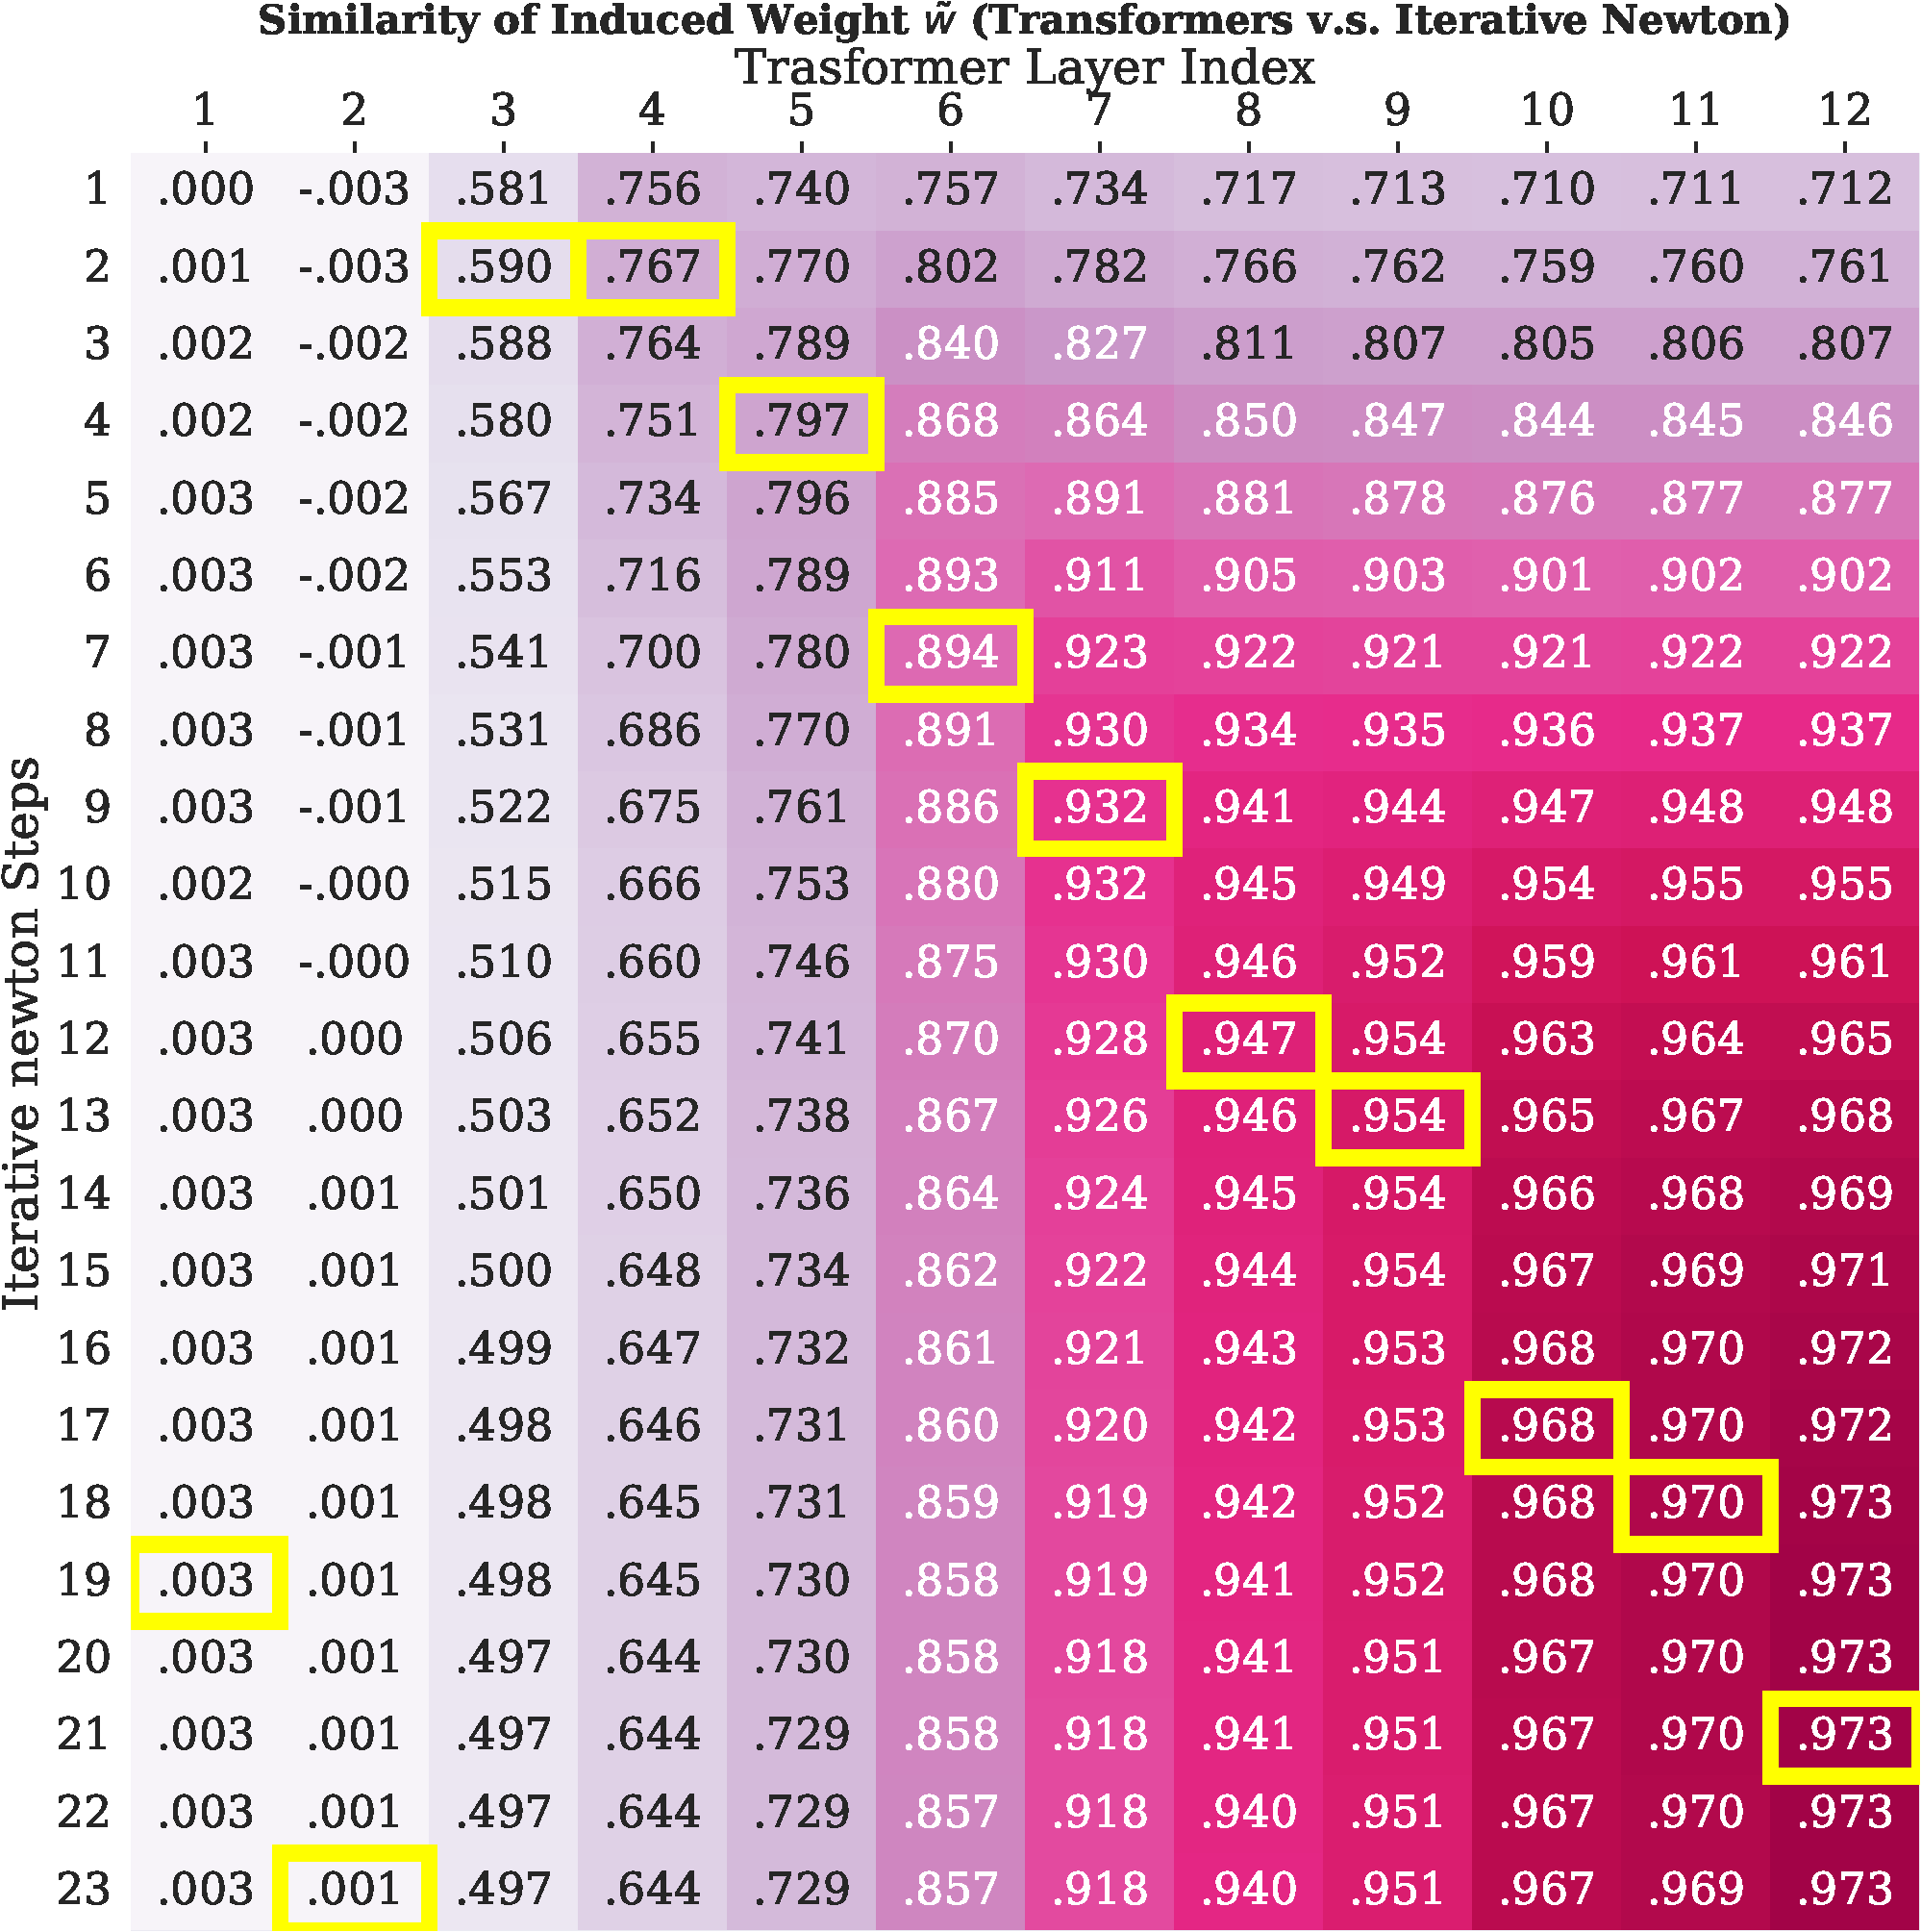
\includegraphics[width=0.45\linewidth]{Figures/12layer_1head/w_sim_heatmap_tf_newton_full.pdf}
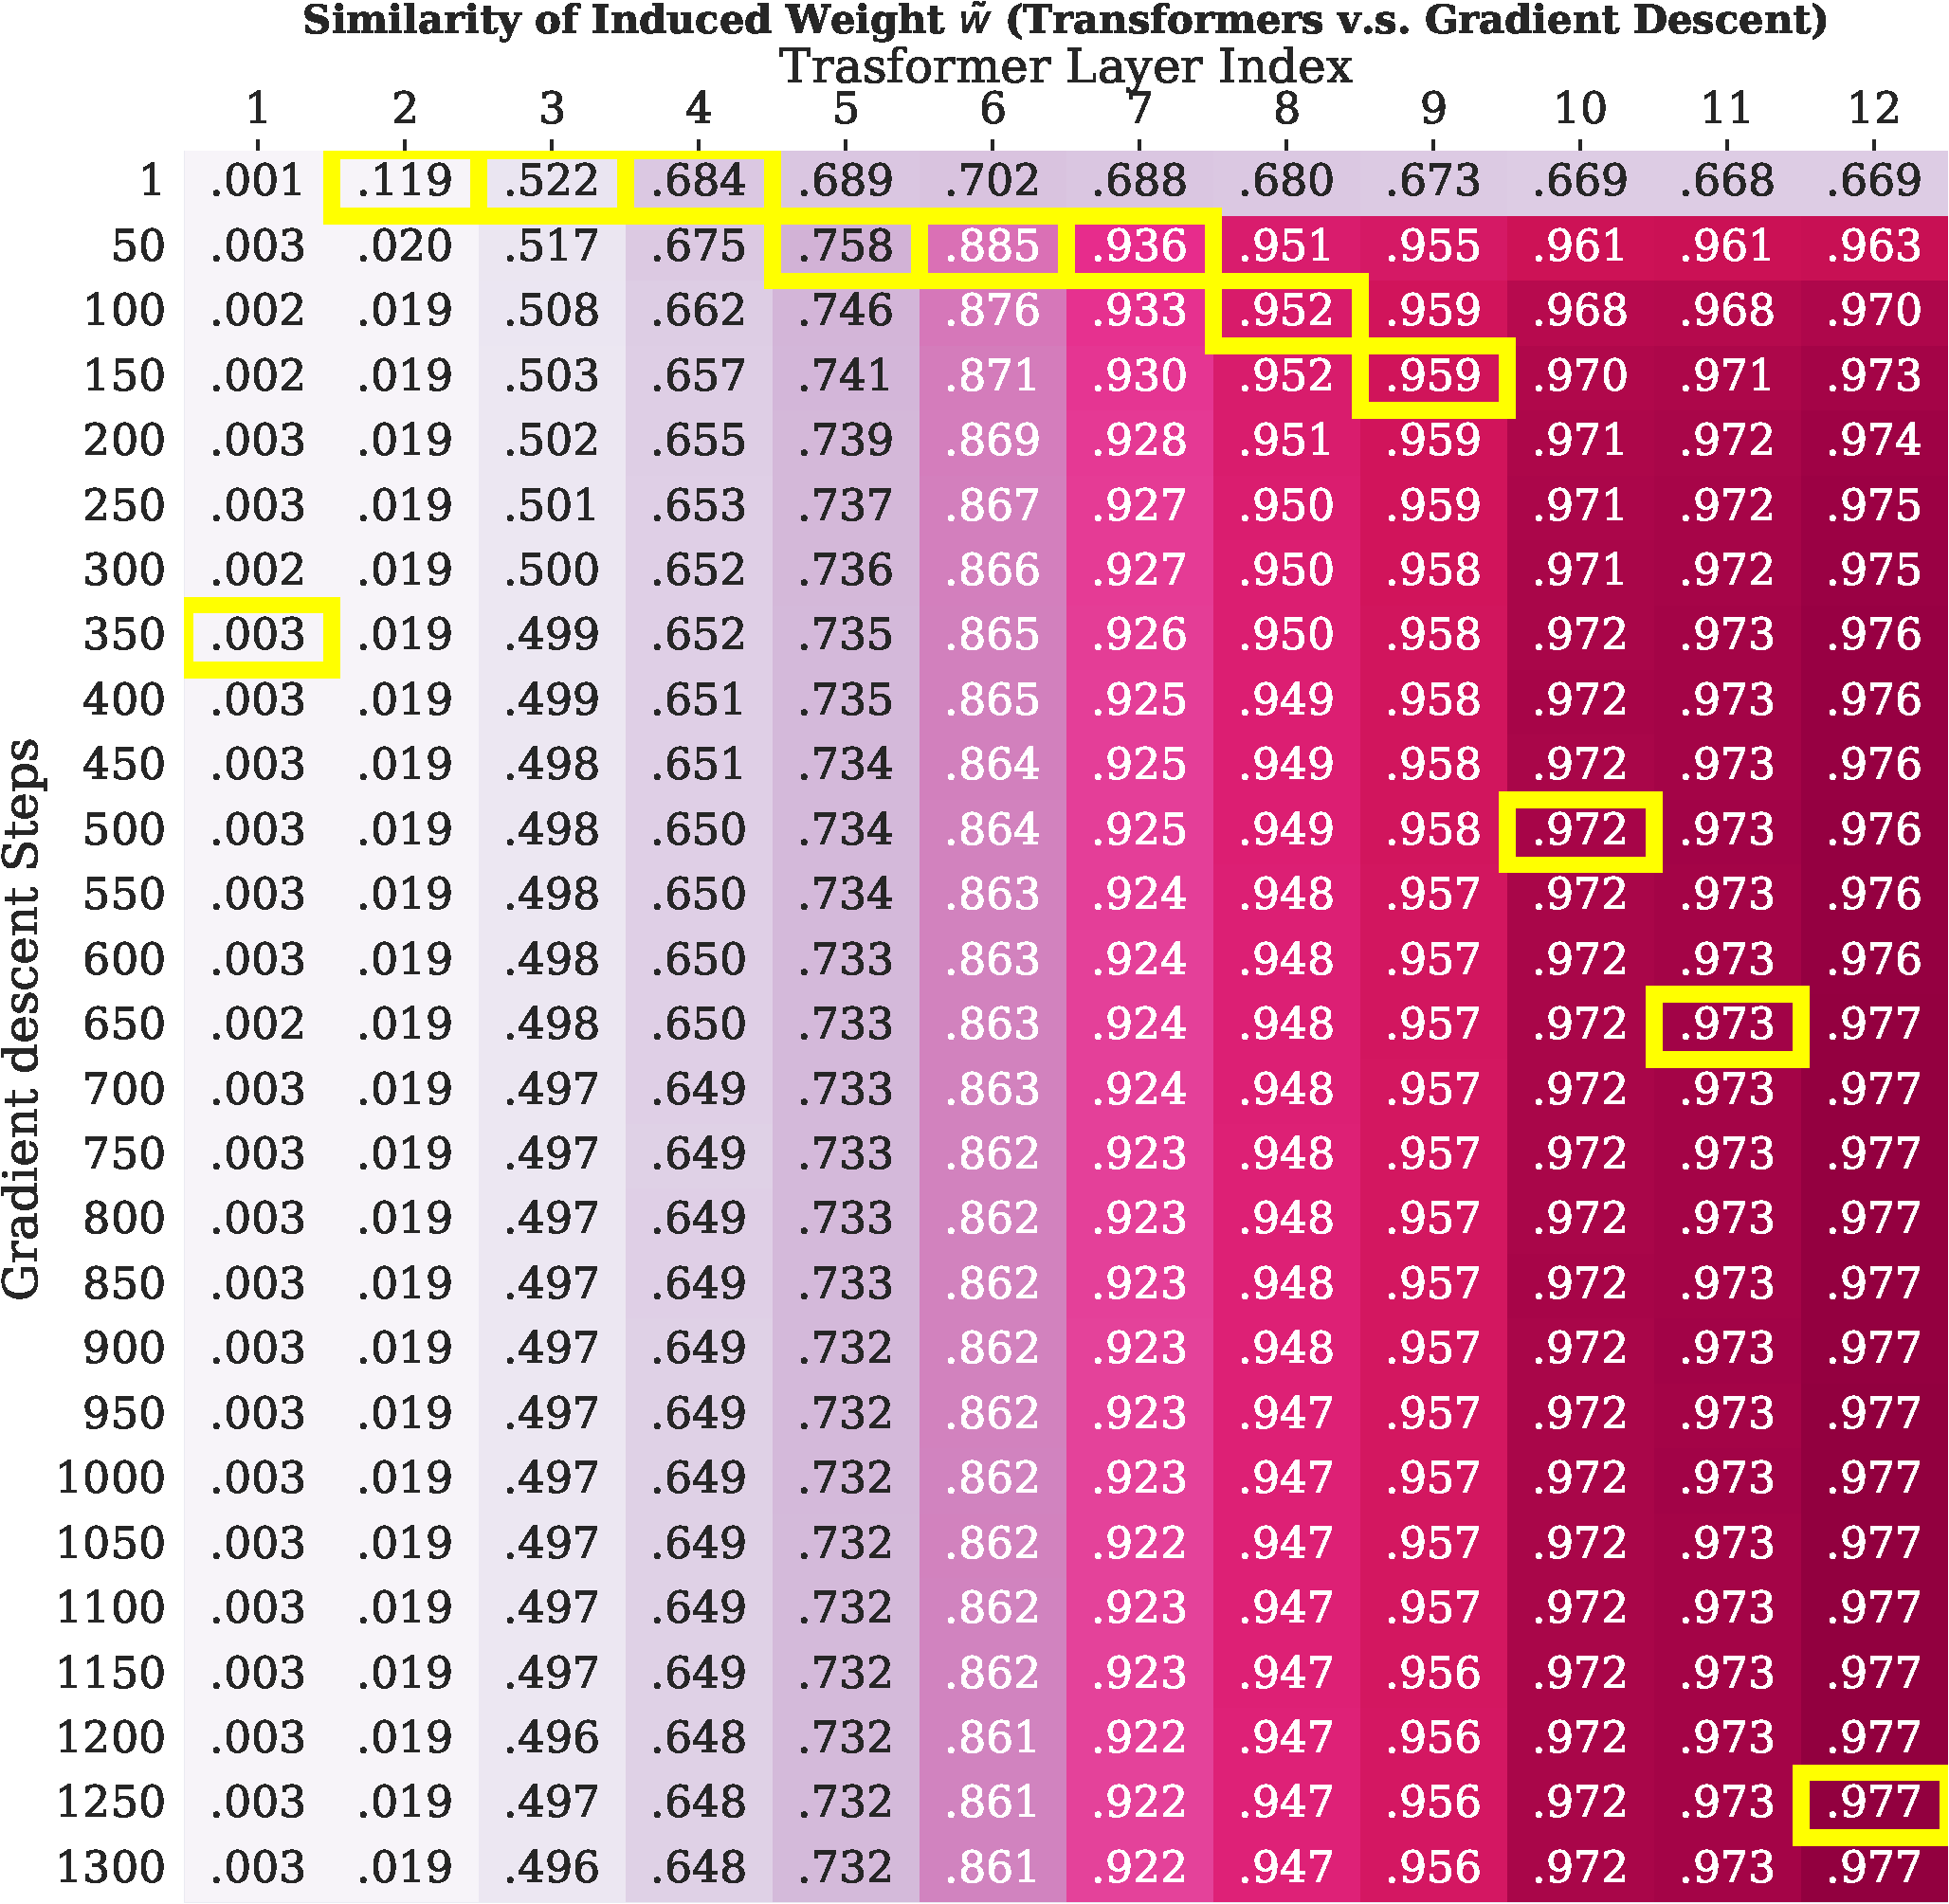
\includegraphics[width=0.45\linewidth]{Figures/12layer_1head/w_sim_heatmap_tf_gd_full.pdf}
\caption{\textbf{Similarity of Induced Weights on an alternative Transformers Configuration.} The best matching steps are highlighted in yellow.} \label{fig:12layer_1head_full_heatmap_sim_w}
\end{figure}

We conclude that our experimental results are not restricted to a specific model configurations, smaller models such as GPT-2 with 12 layers and 1 head each layer also suffice in implementing the \newton's method, and more similar than gradient descents, in terms of rate of convergence. 

\subsubsection{Experiments on Transformers with More Layers} \label{app:24-layer}
In this section, we investigate whether deeper models would behave similarly or differently. We work on Transformers with 24 layers and 8 heads each. 

\begin{figure}[!htp]
    \centering
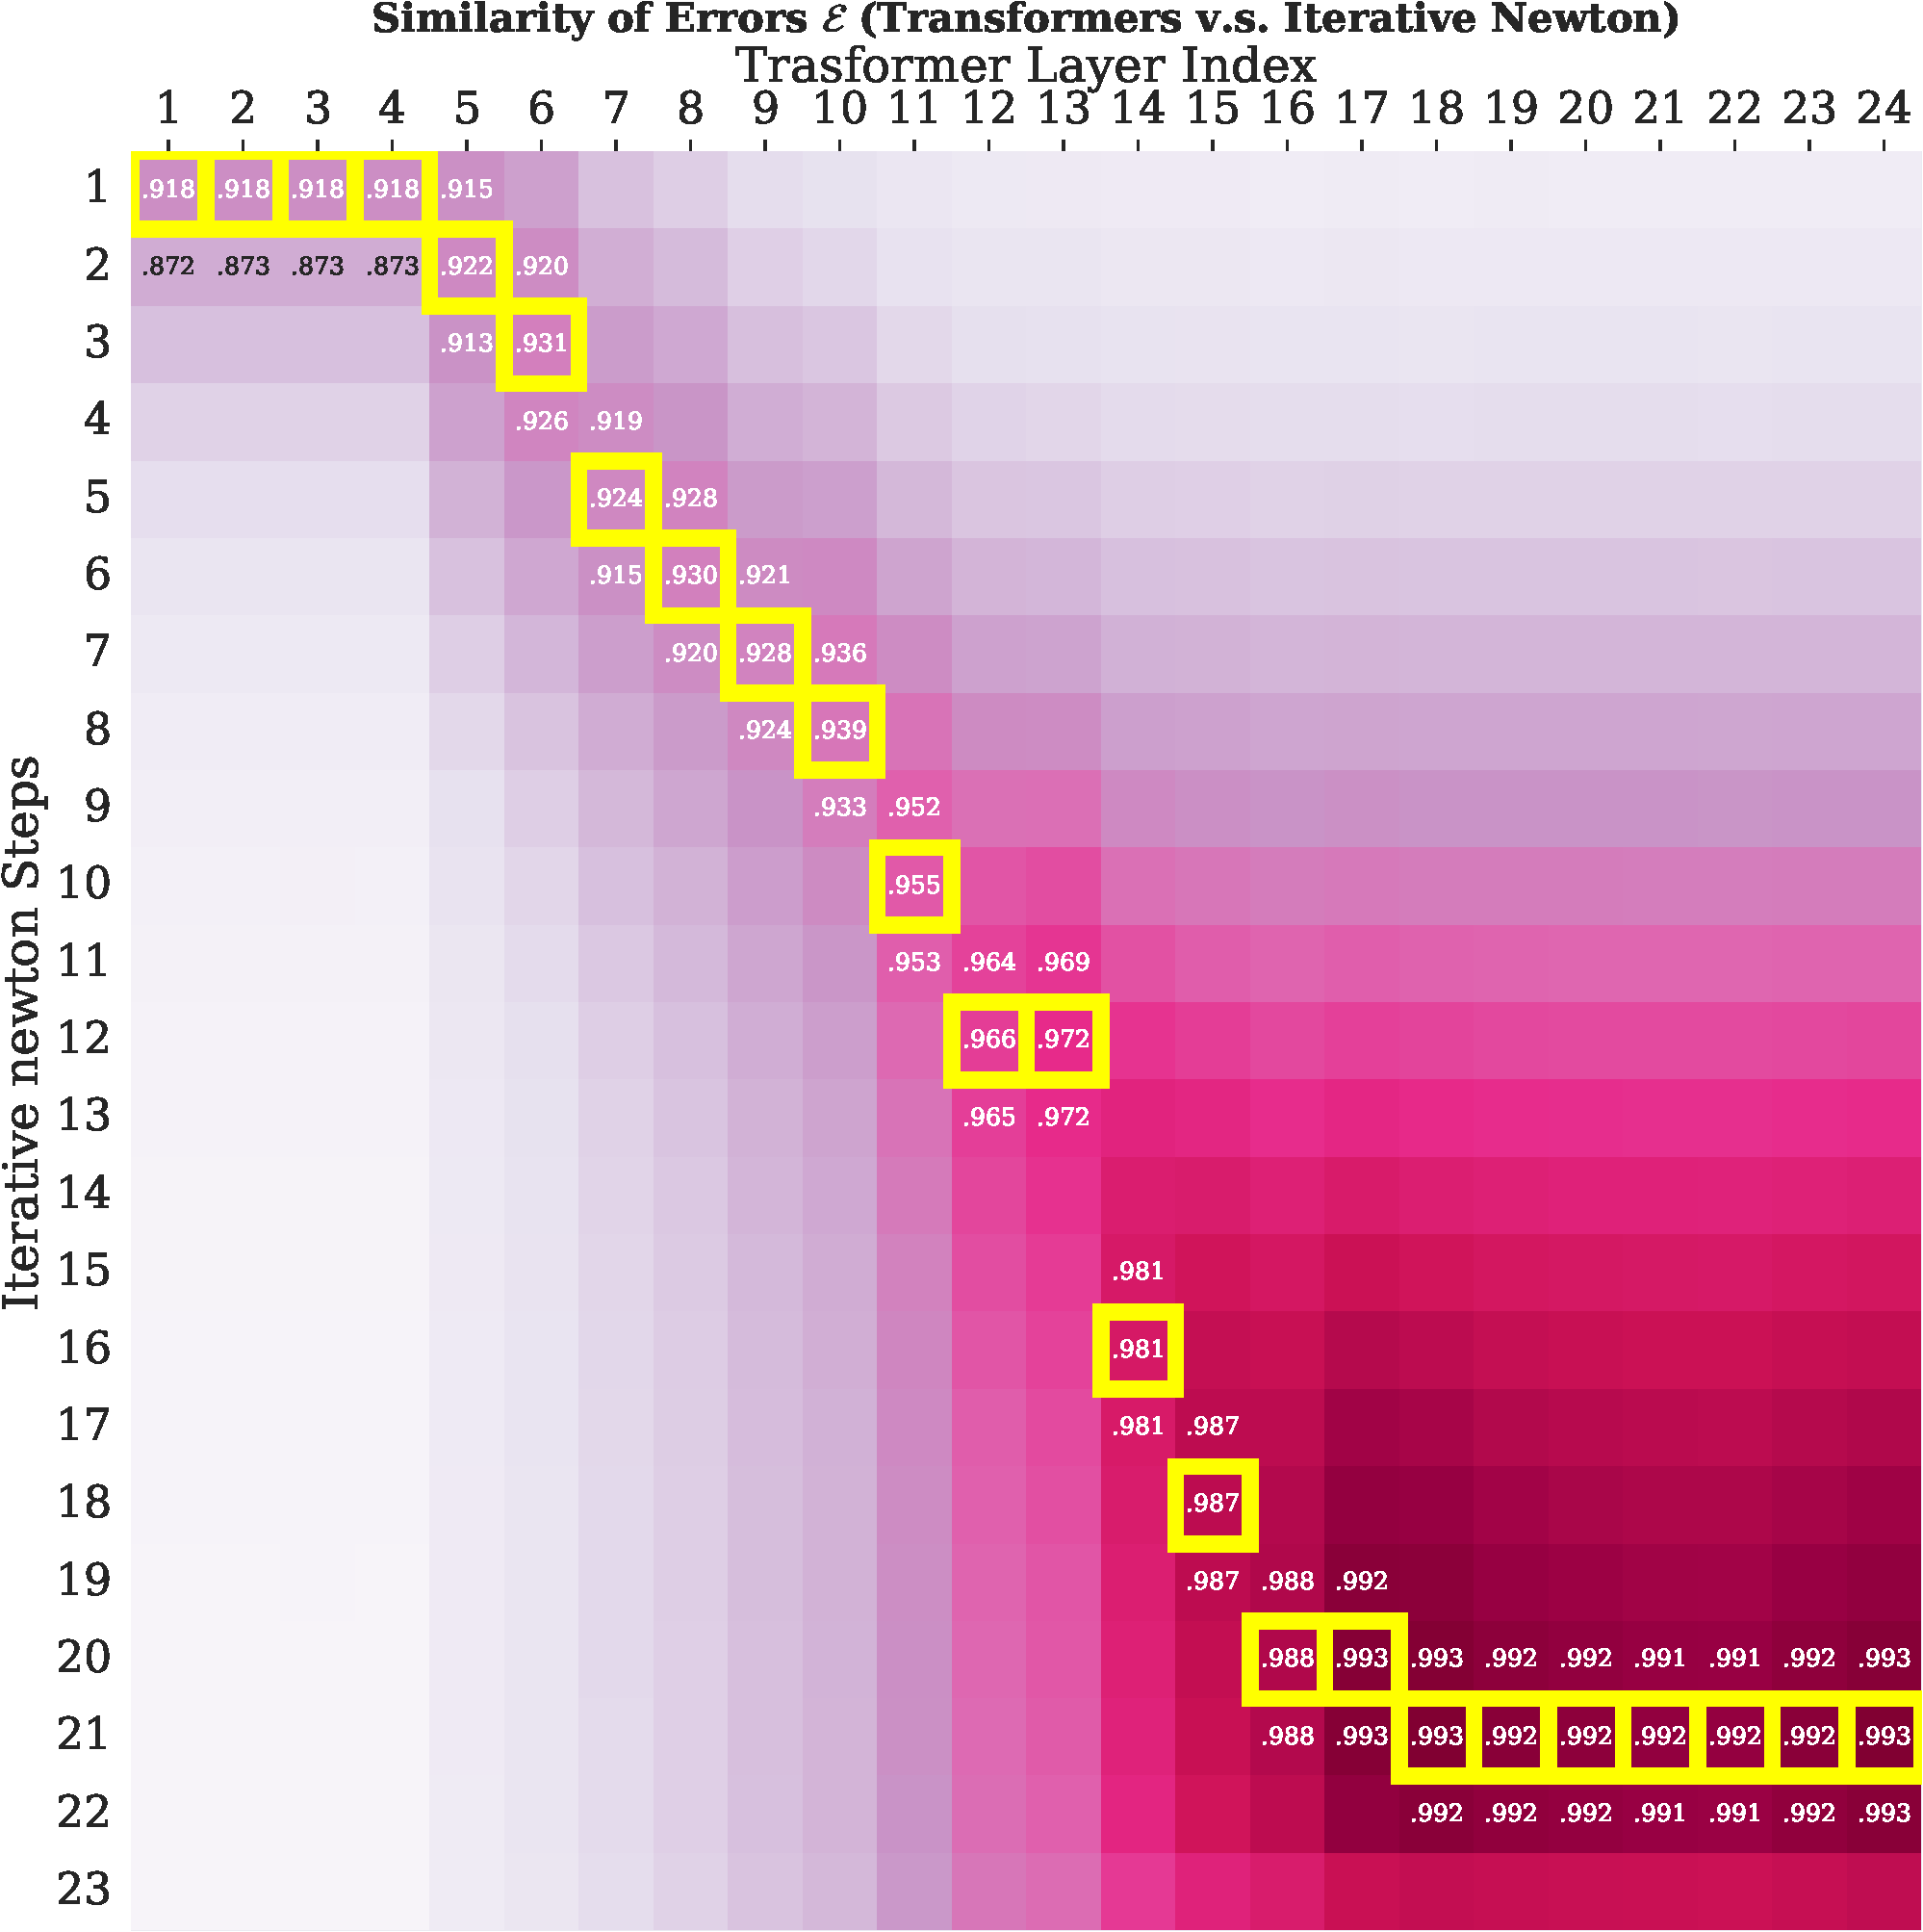
\includegraphics[width=0.45\linewidth]{Figures/24layer_8head/24layer_resid_sim_heatmap_tf_newton.pdf}
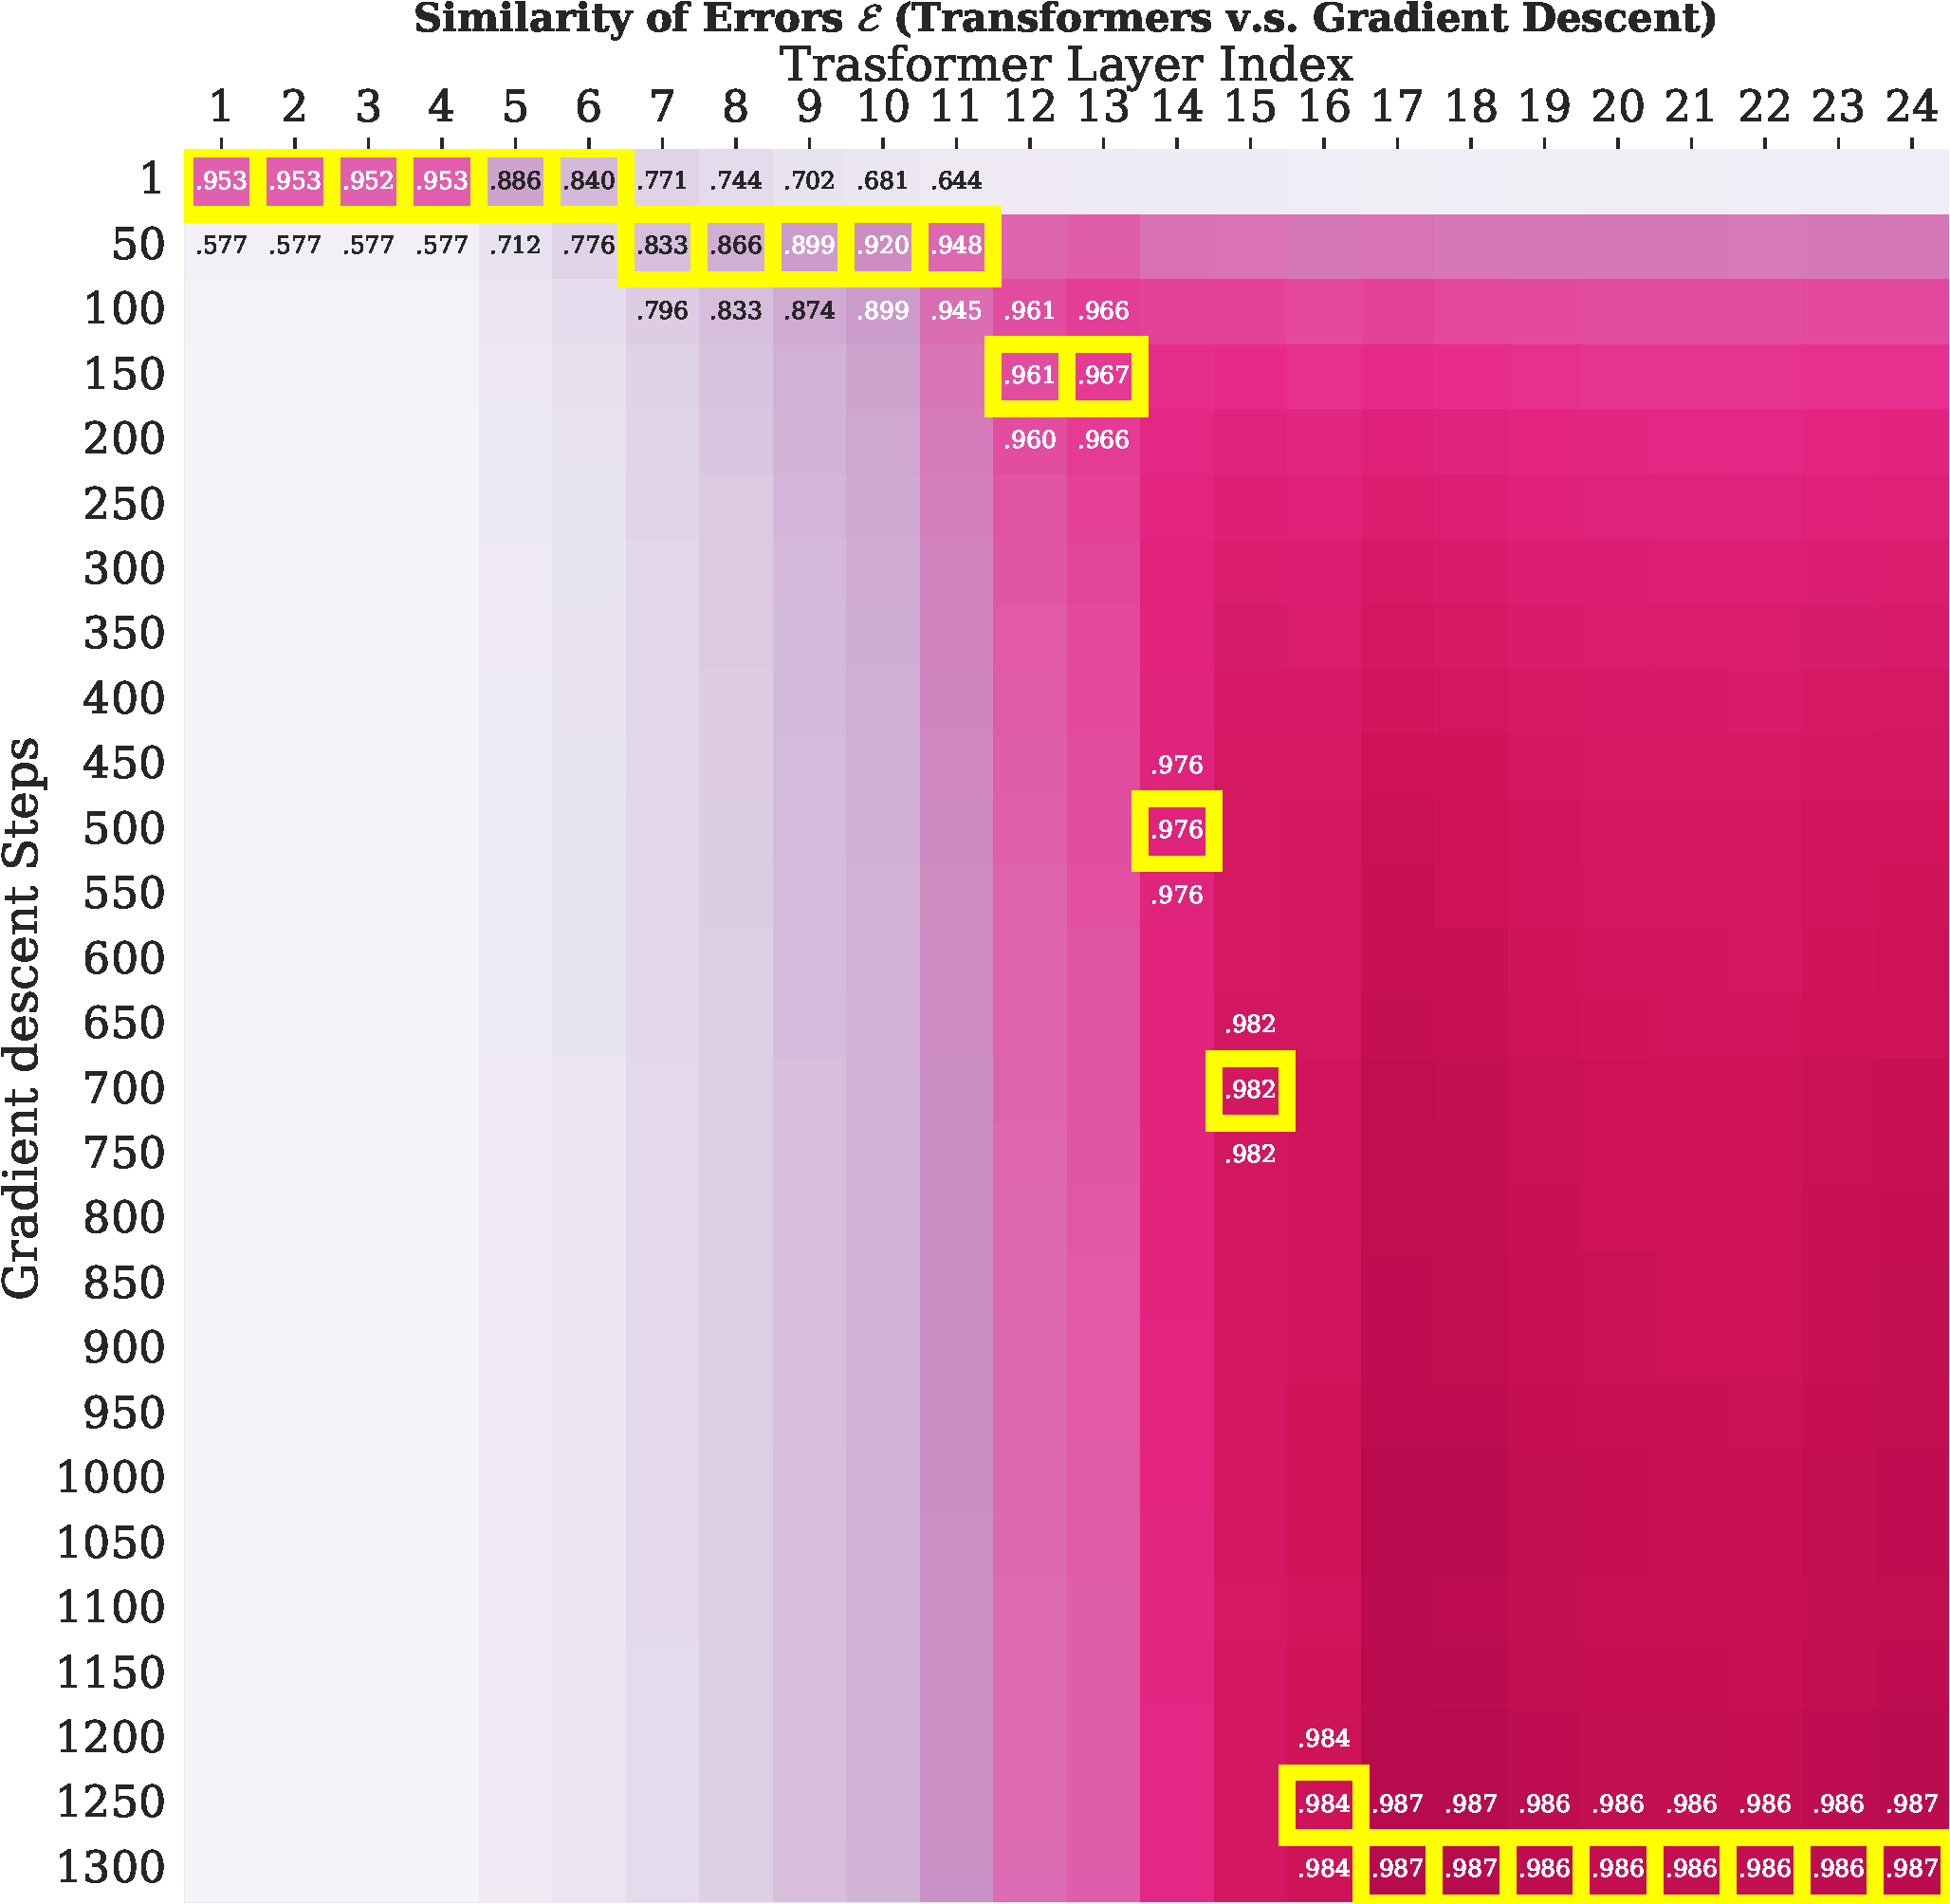
\includegraphics[width=0.45\linewidth]{Figures/24layer_8head/24layer_resid_sim_heatmap_tf_gd.pdf}
\caption{\textbf{Similarity of Errors on a 24-layer Transformers Configuration.} The best matching steps are highlighted in yellow. } \label{fig:24layer_full_heatmap_sim_e}
\end{figure}

\begin{figure}[!htp]
    \centering
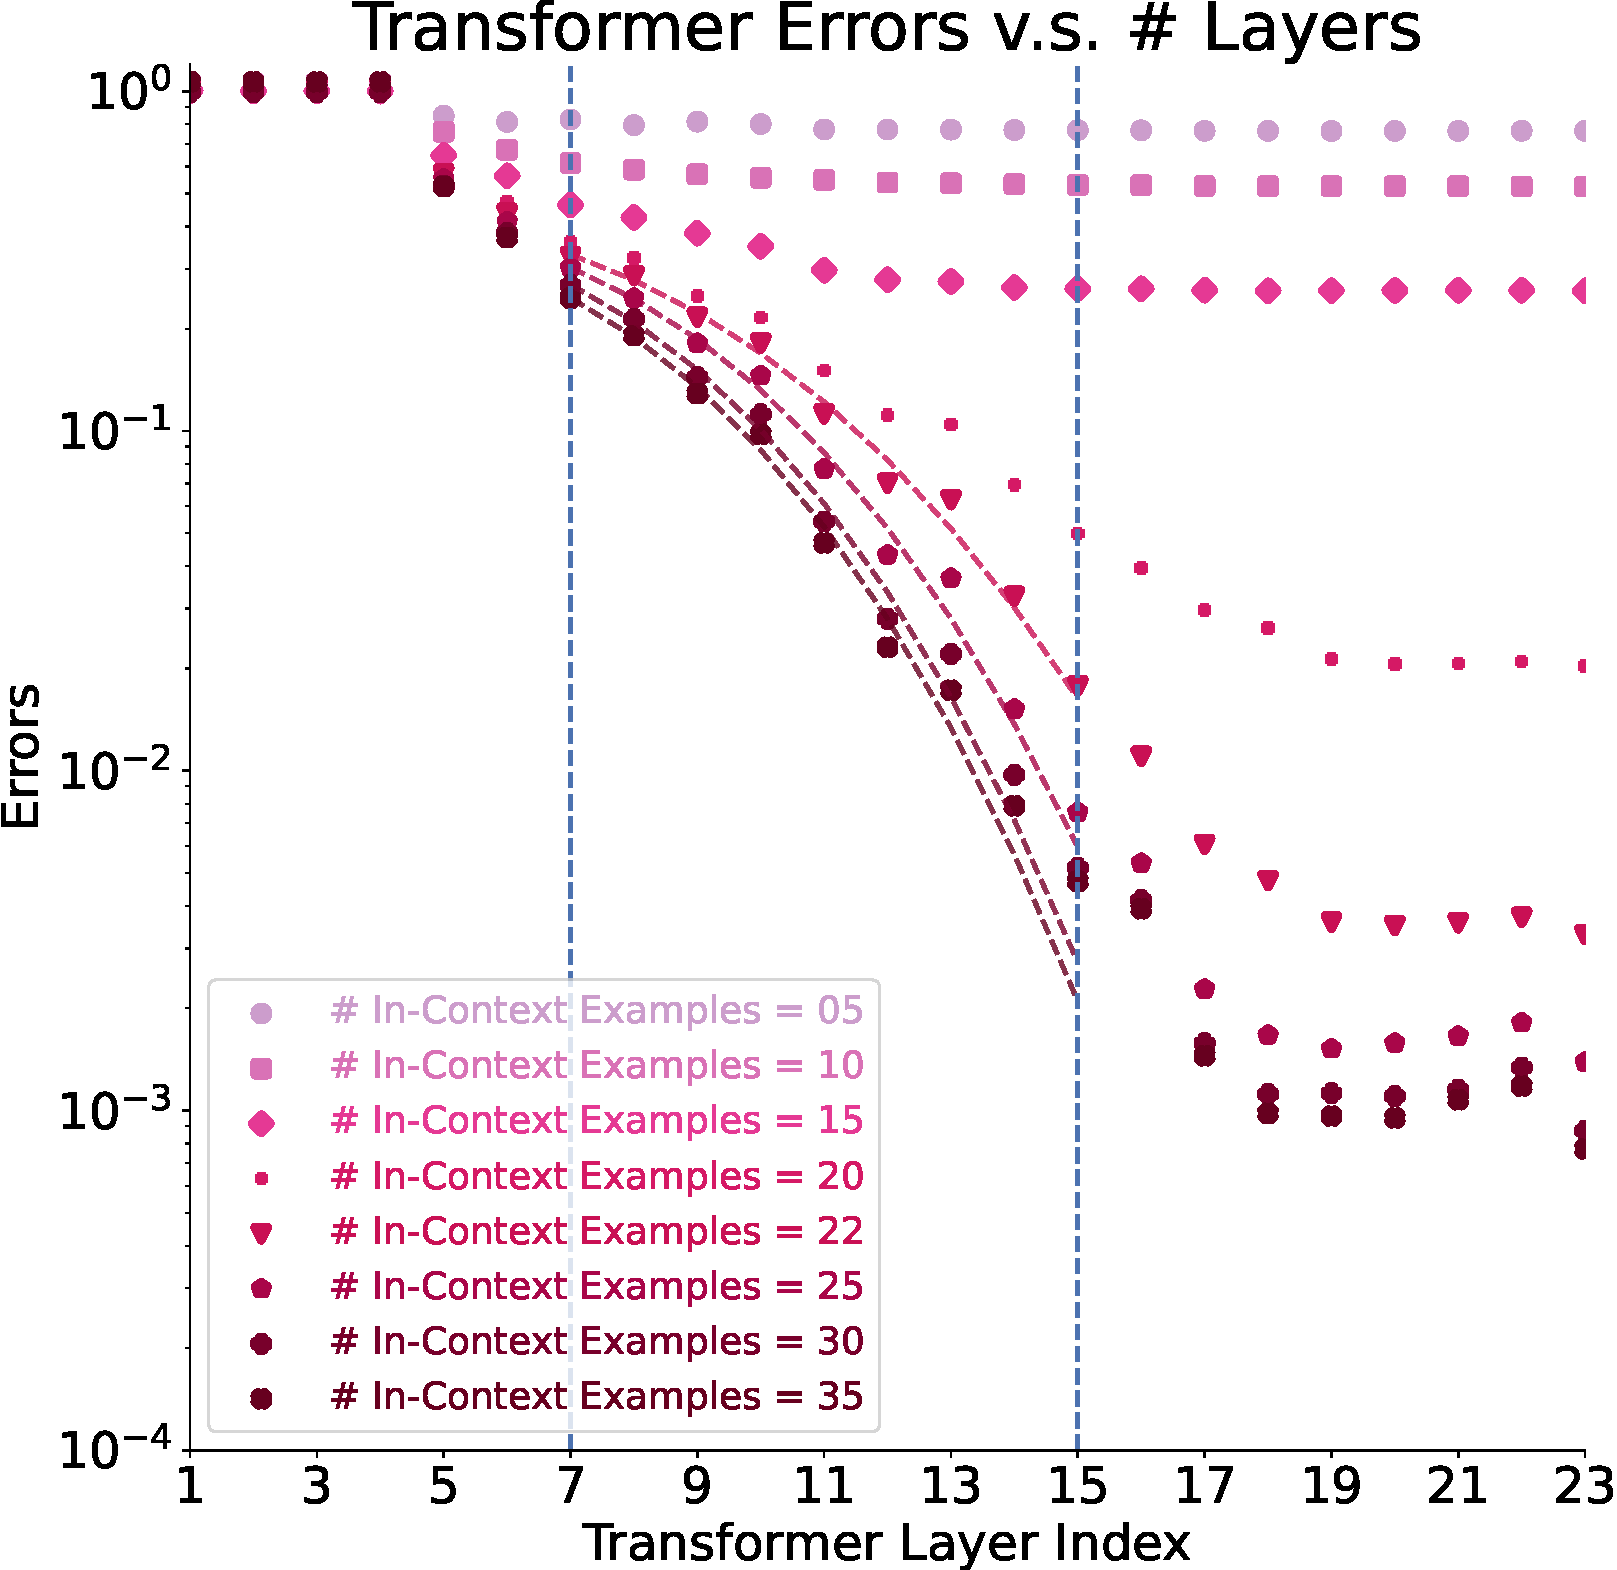
\includegraphics[width=0.45\linewidth]{Figures/24layer_8head/transformers__24layer_8head_error_new.pdf}
    \caption{Transformers with 24 layers also converge superlinearly, similar to \newton.}
    \label{fig:convergence-24layer}
\end{figure}

\clearpage
\subsection{Heatmaps with Best-Matching Steps Help Compare Convergence Rates} \label{app:best-match}
{In this section, we show the heatmaps with best-matching steps among \textit{known algorithms.}}
\begin{figure}[!htp]
    \centering
    \subfigure[\newton\ v.s. \gd]{
    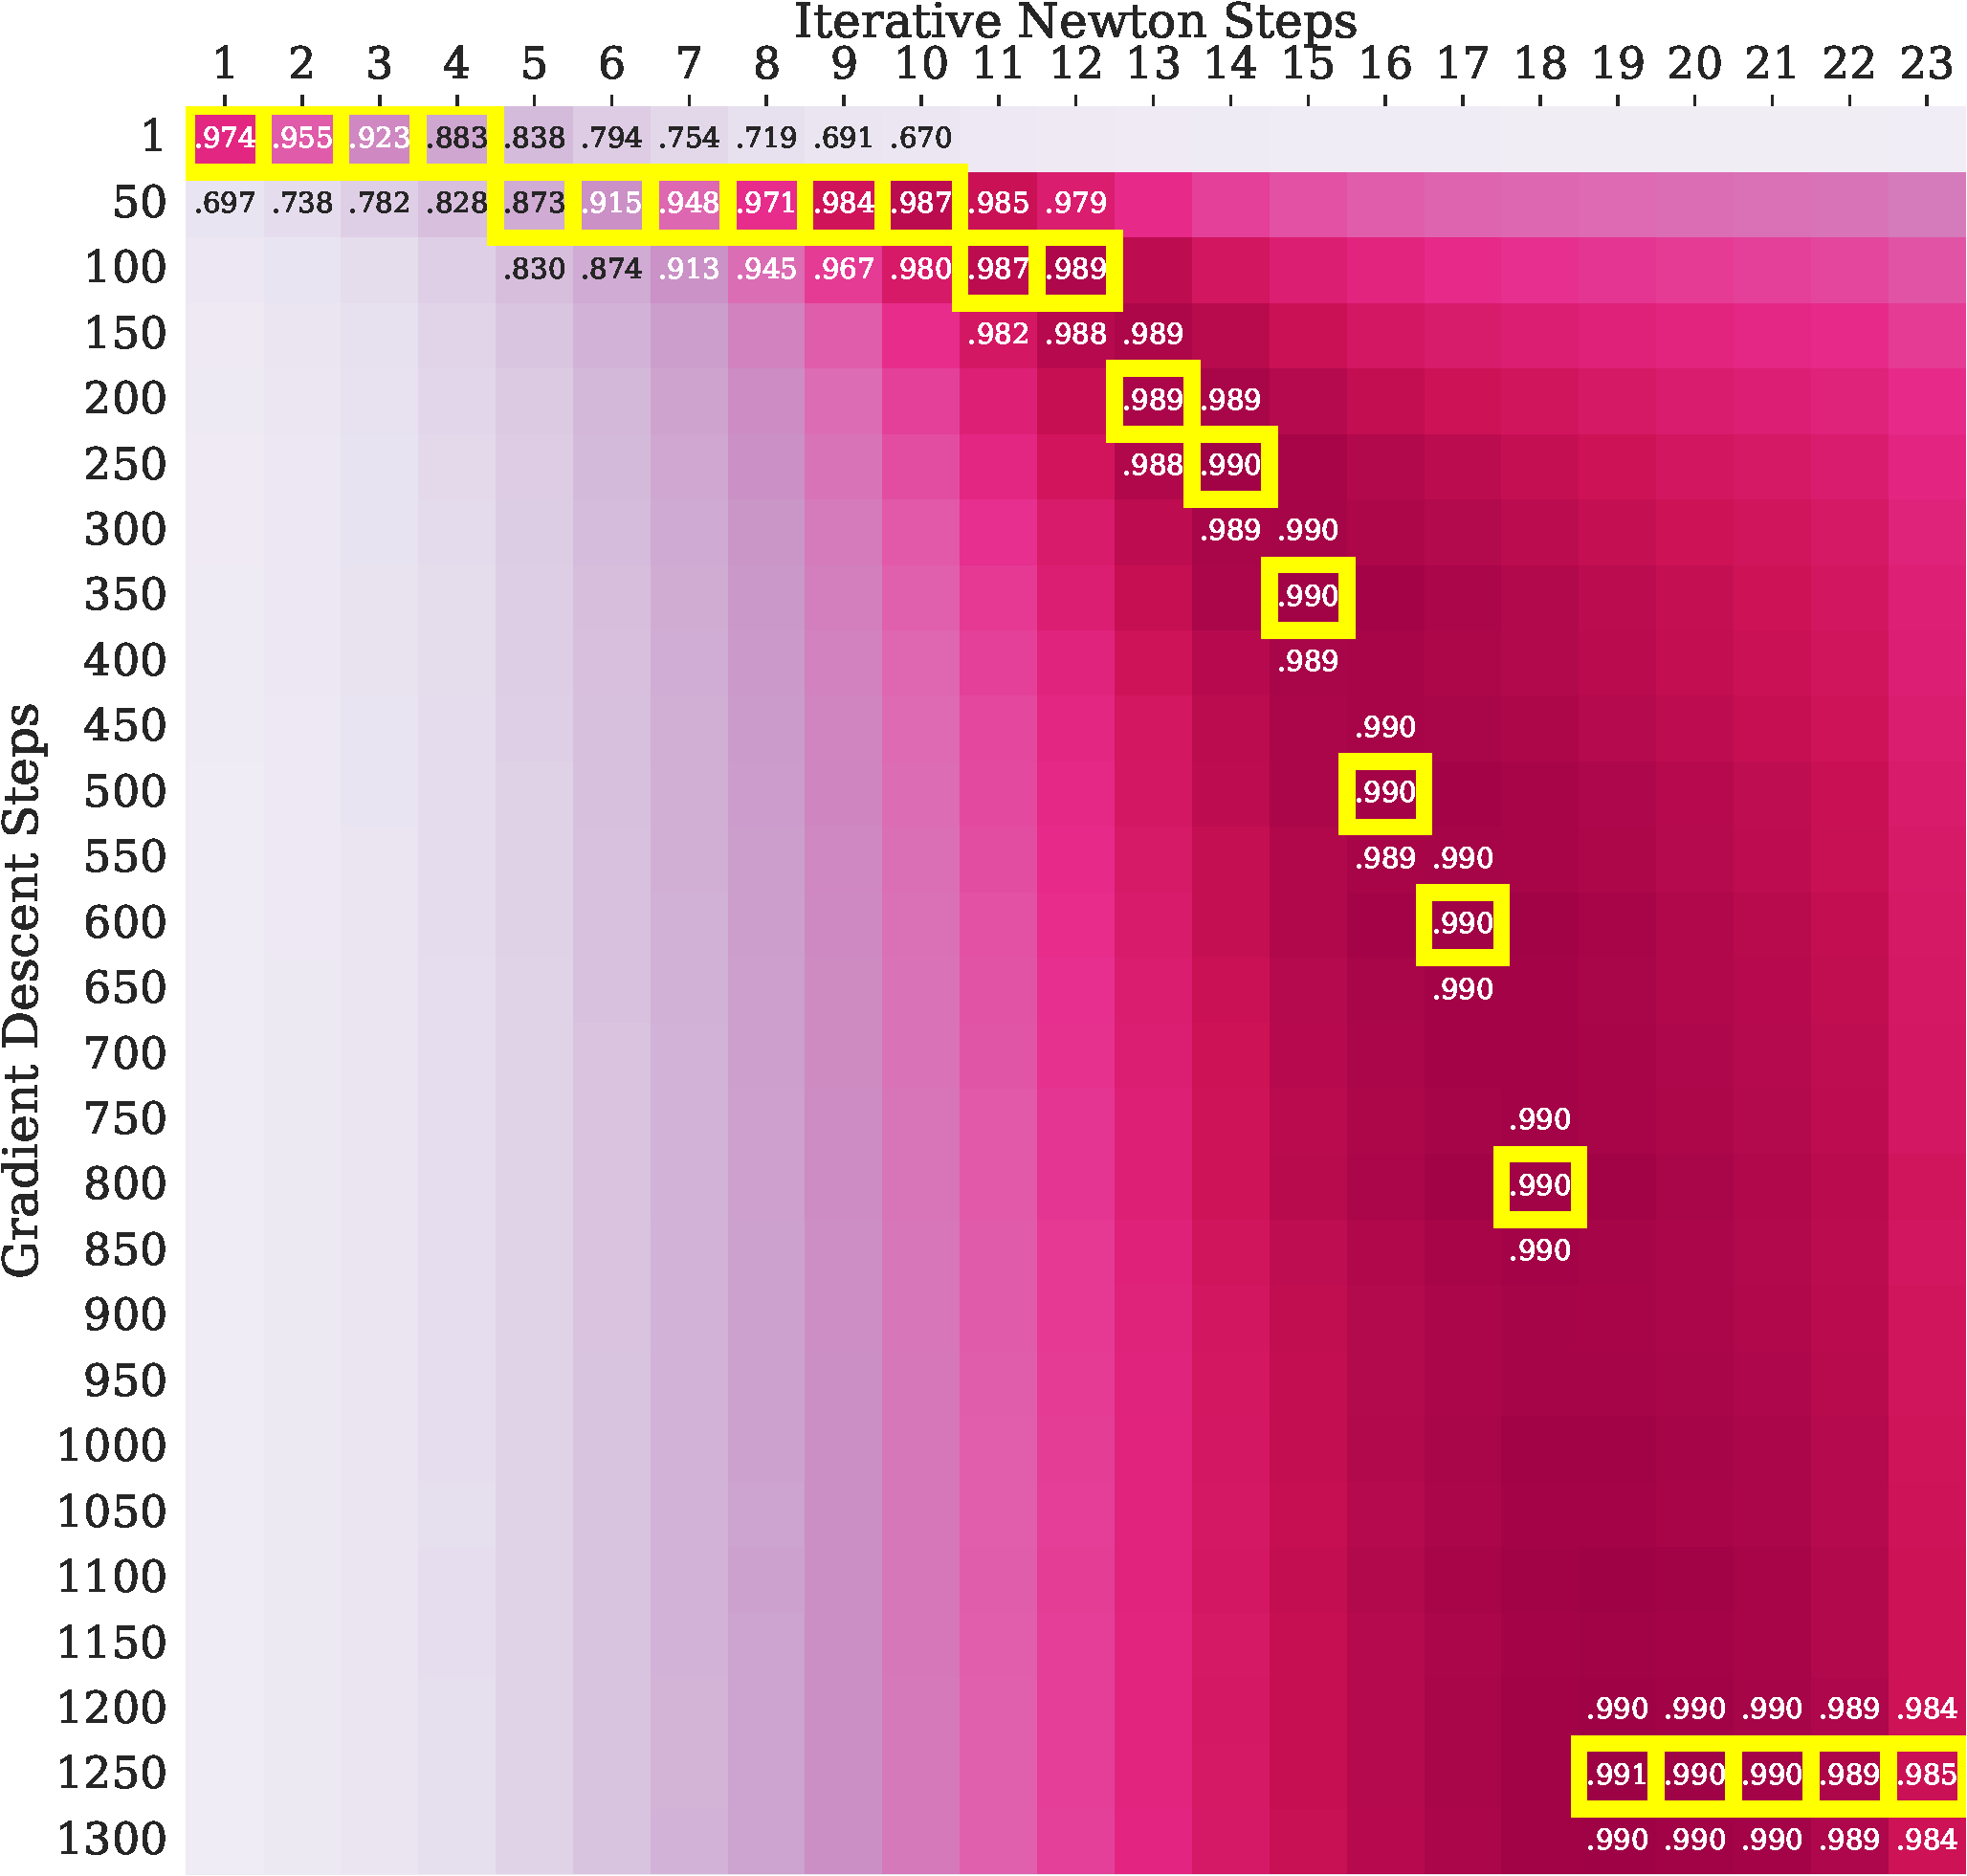
\includegraphics[width=0.45\linewidth]{Figures/convergence/gd_newton.pdf}
    }
    \subfigure[\newton\ v.s. \newton]{
    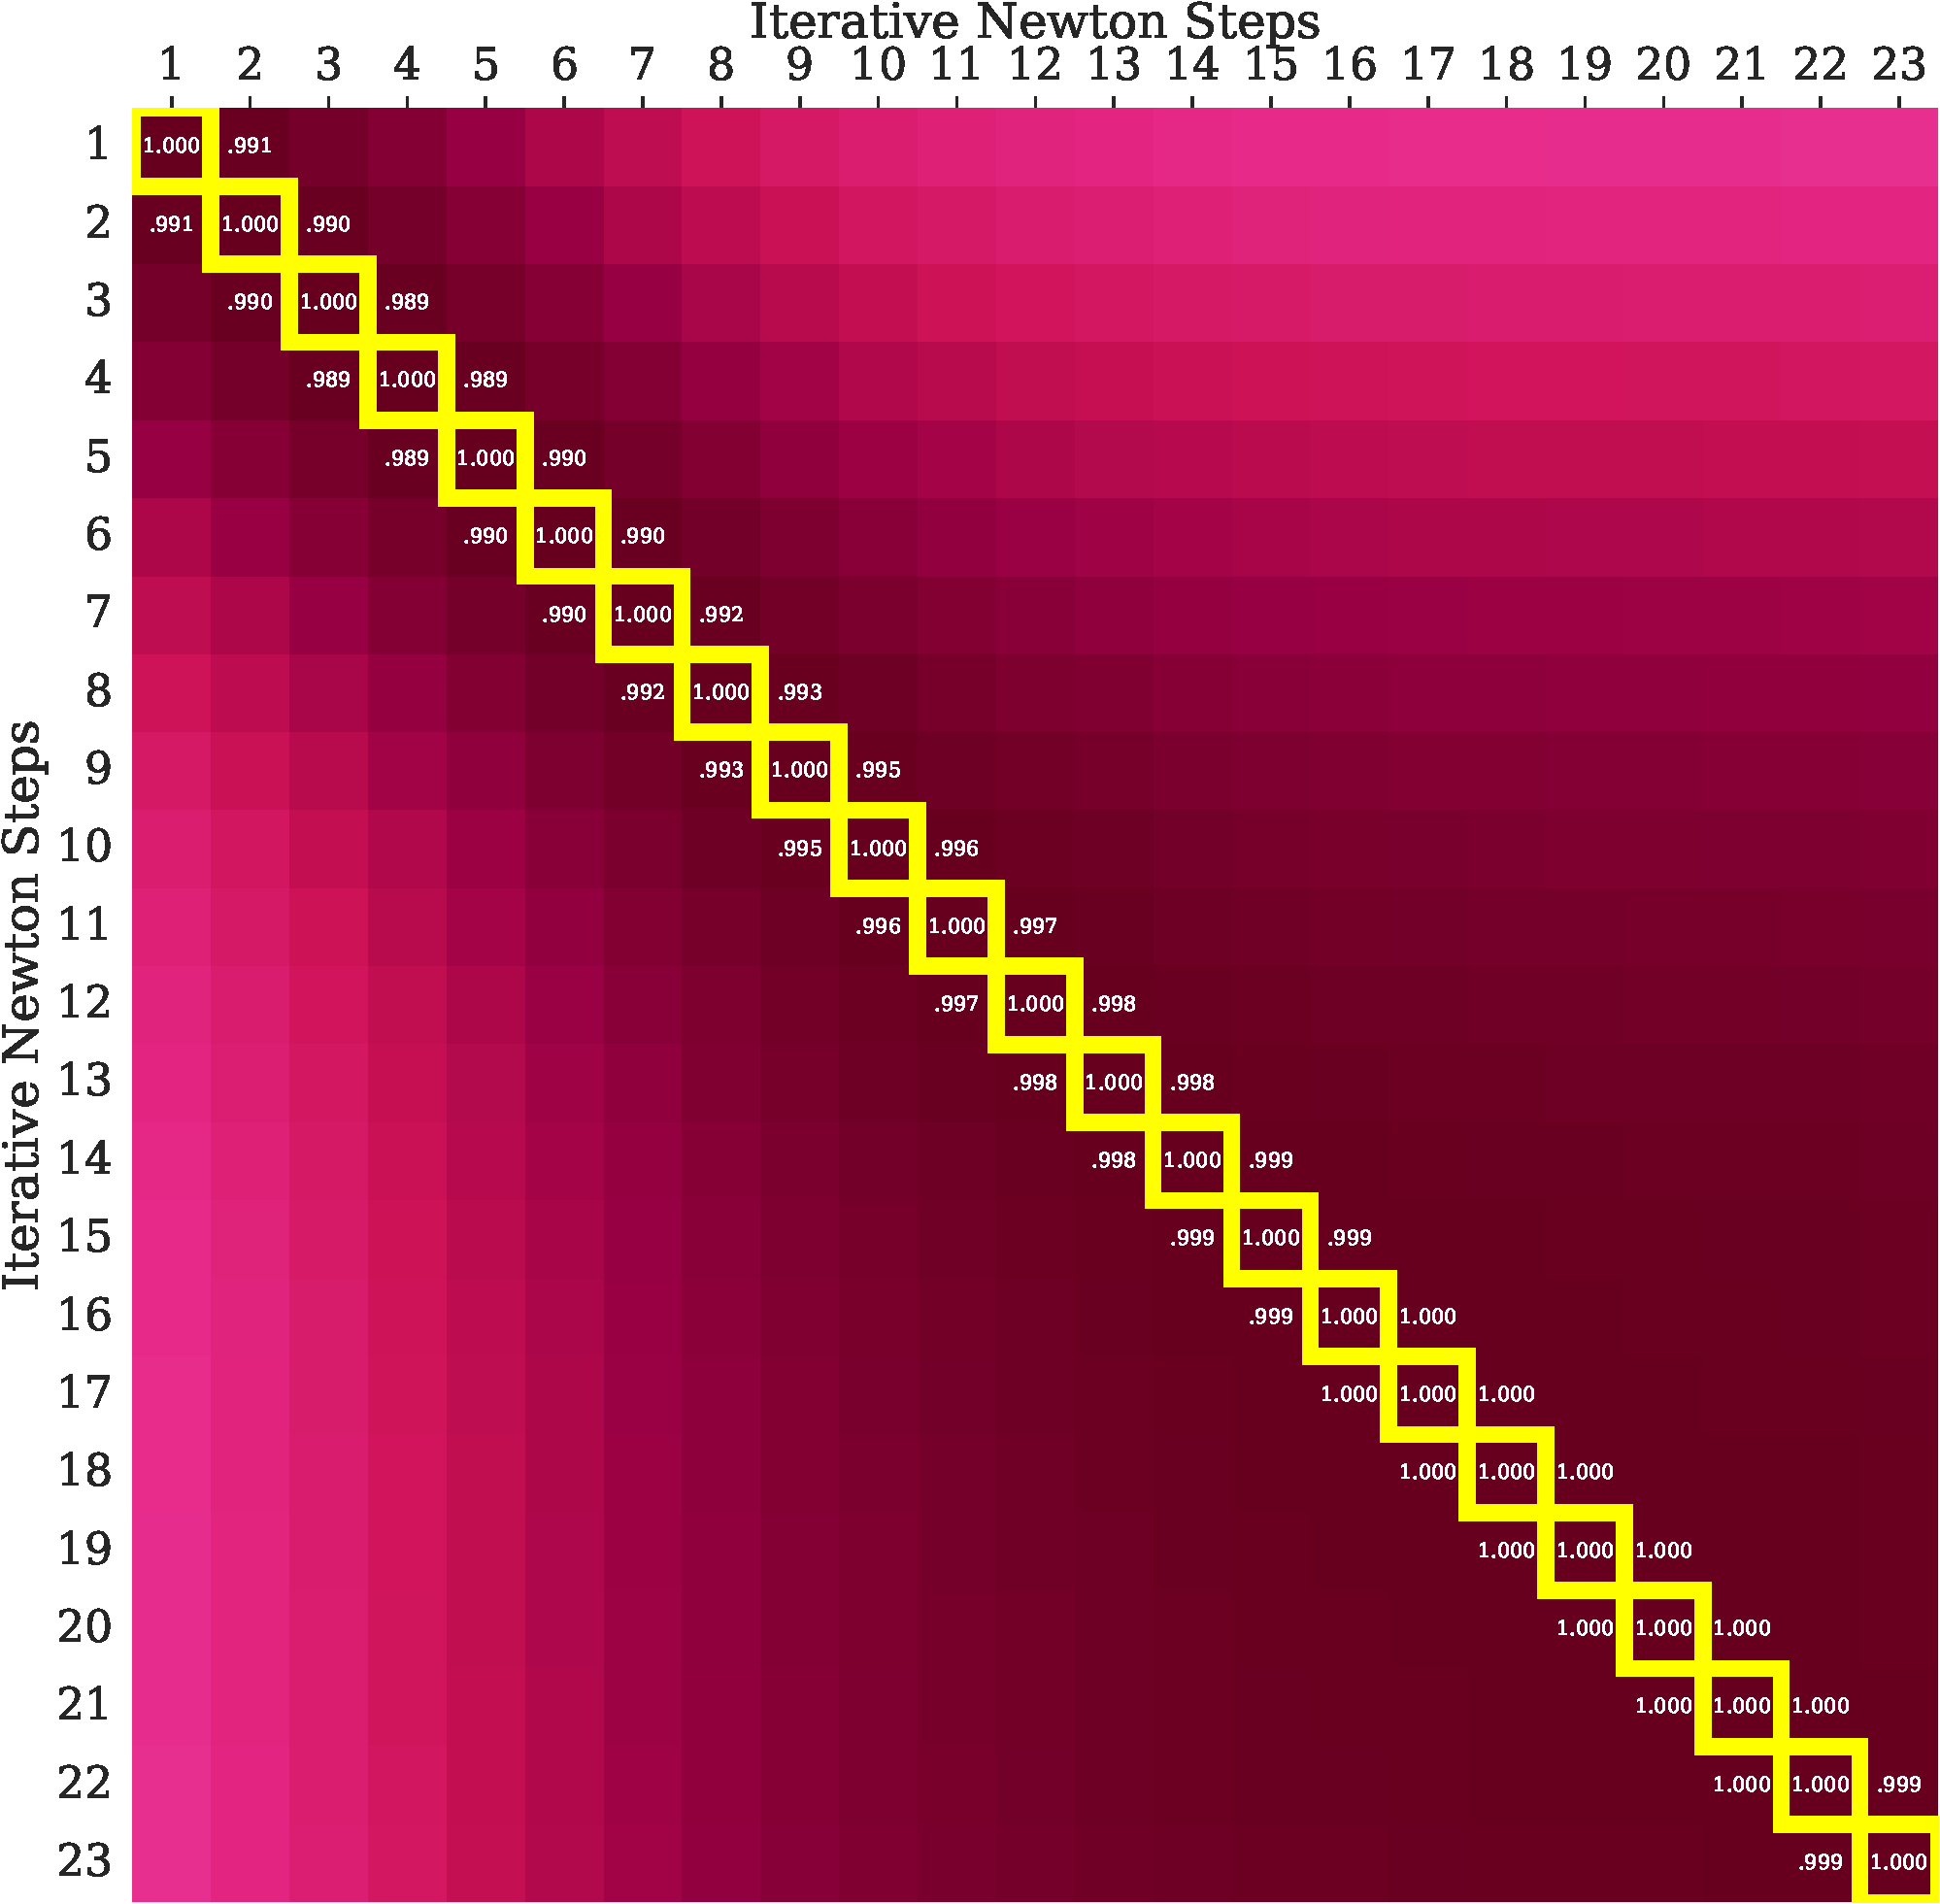
\includegraphics[width=0.45\linewidth]{Figures/convergence/newton_newton.pdf}
    }
    \subfigure[\newton\ v.s. BFGS]{
    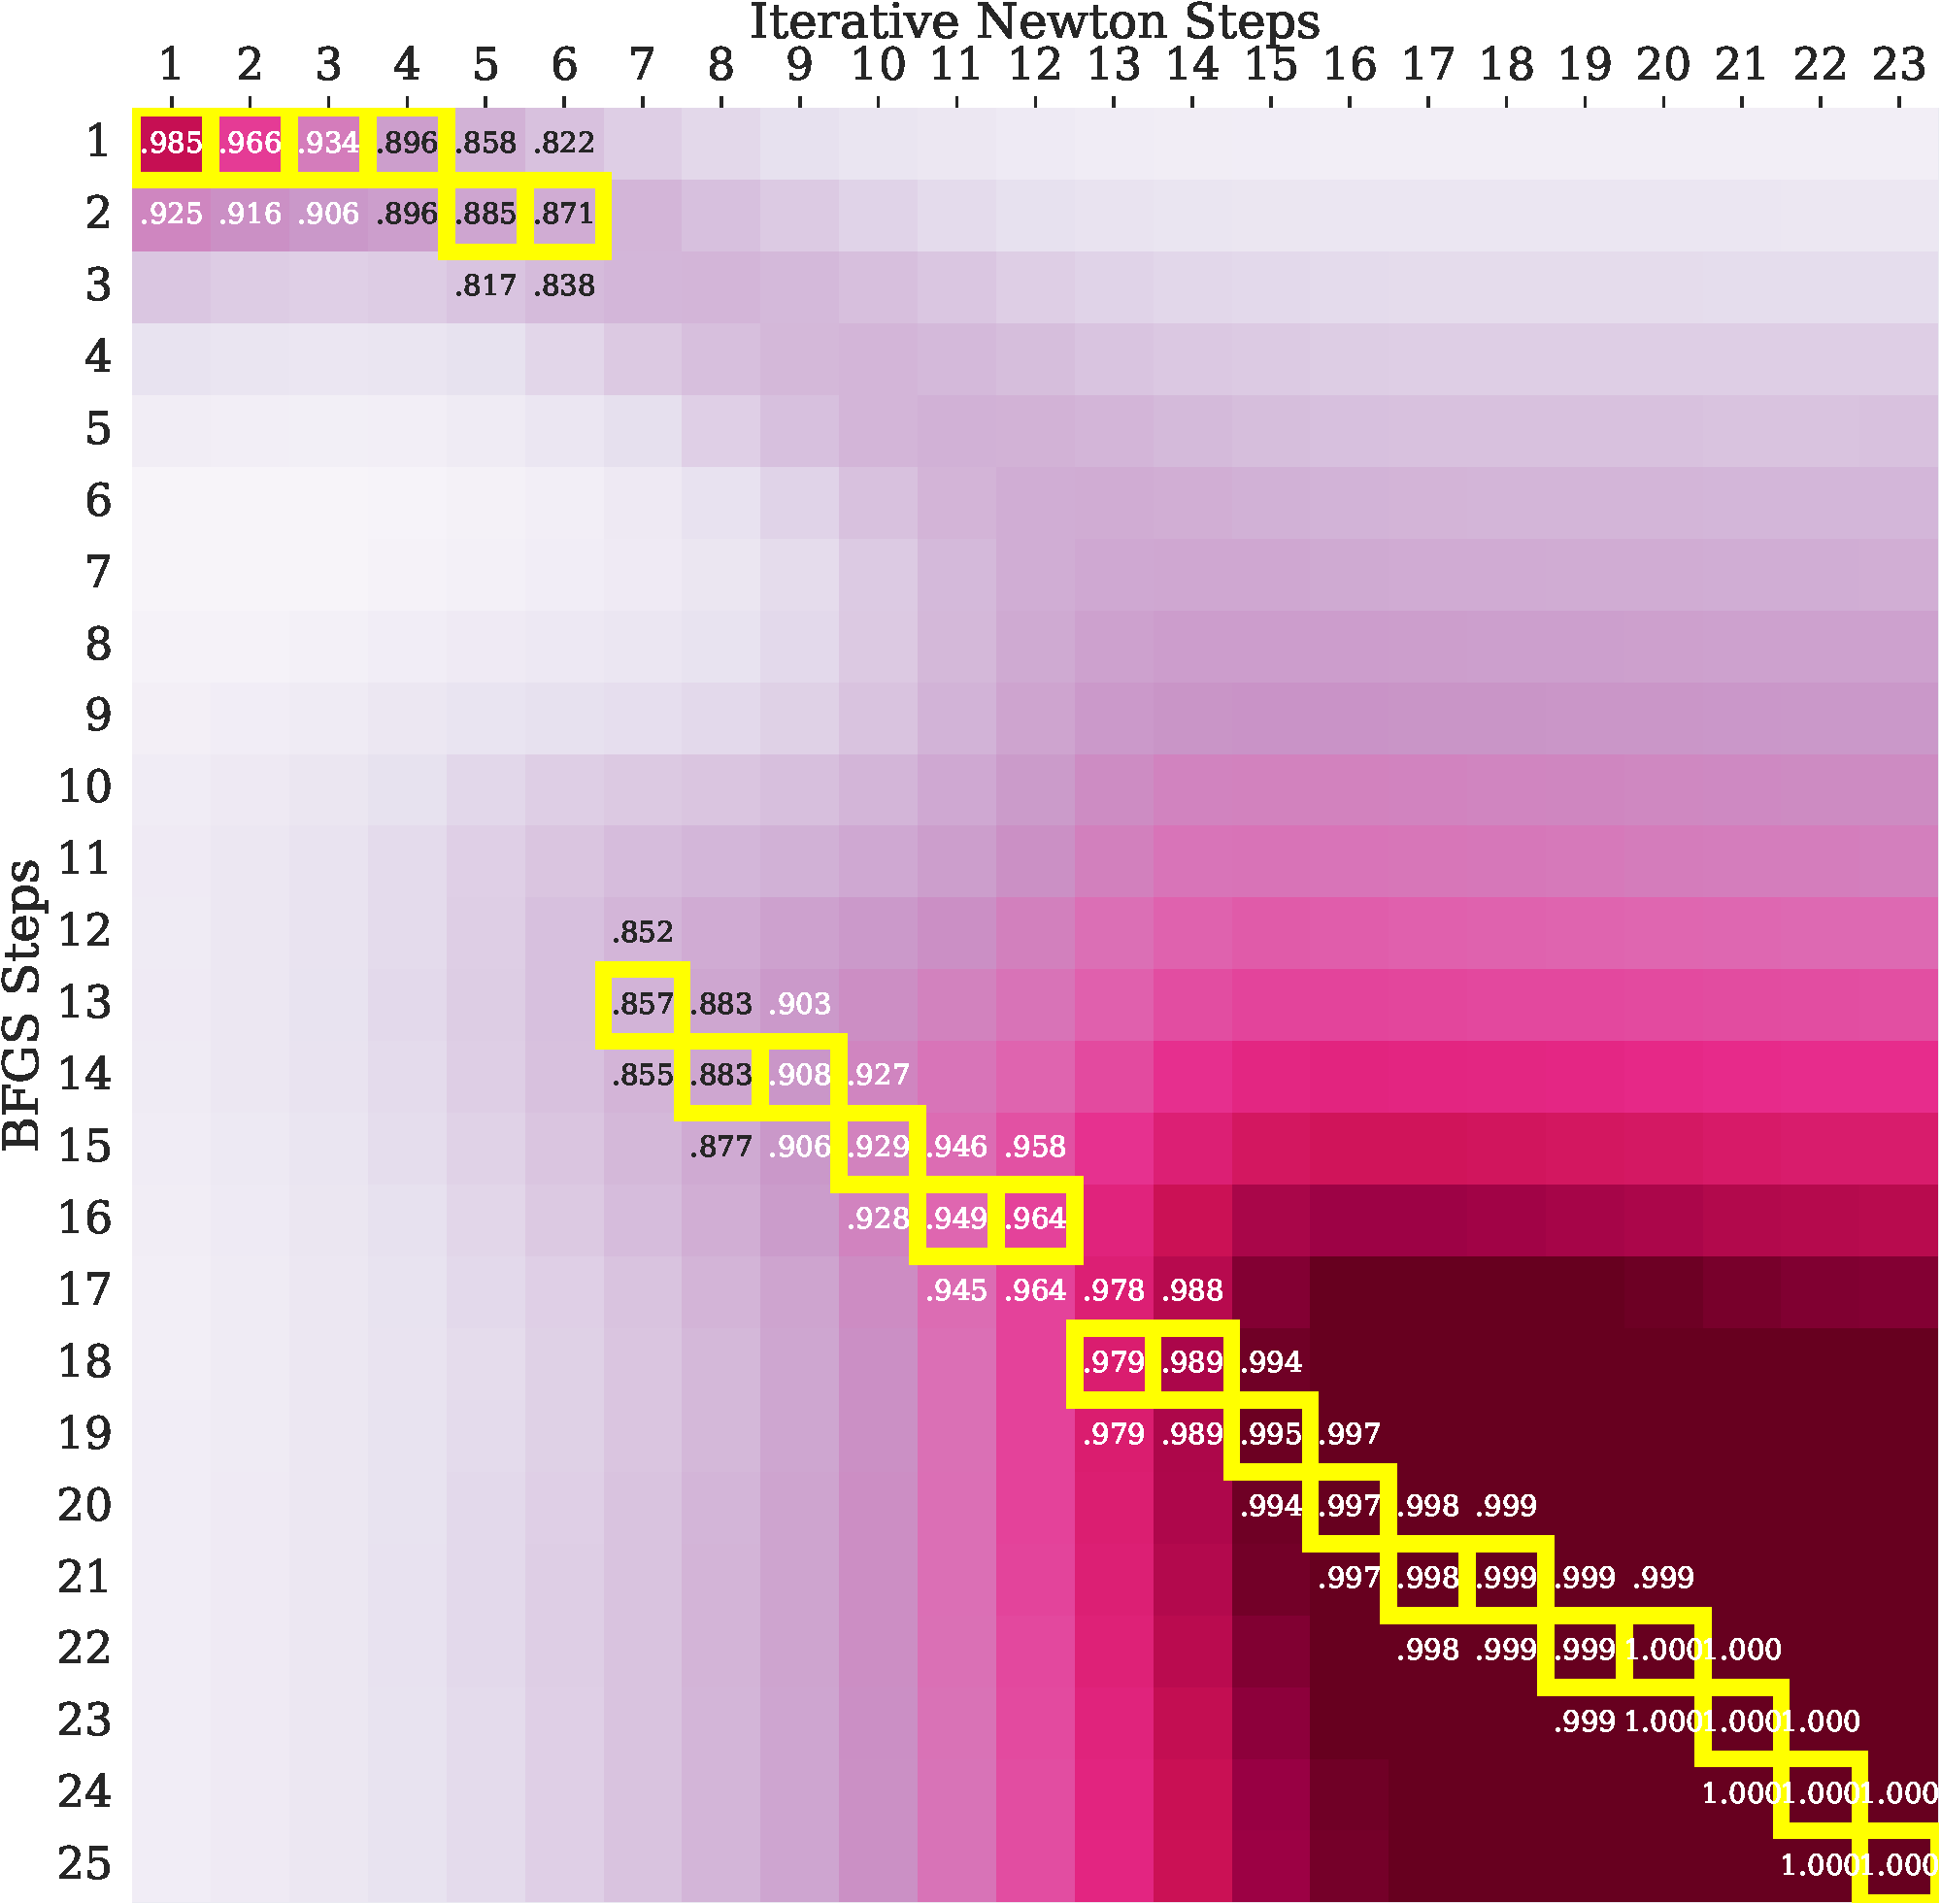
\includegraphics[width=0.45\linewidth]{Figures/convergence/bfgs_newton.pdf}
    }
    \caption{Best-Matching Steps on Similarity of Residuals Help Compare Convergence Rates. (a: top-left) When comparing \newton\ and \gd, there is an exponential trend -- showing \newton\ converges exponentially faster than \gd. (b: top-right) When \newton\ is compared with itself in sub-figure, there is a linear trend -- showing they have the same convergence rate. (c: bottom) When \newton\ is compared to BFGS in sub-figure, there a linear trend after there are enough steps for BFGS to approximate second-order information -- showing \newton\ and BFGS share a similar convergence rate after sufficient BFGS steps.}
    \label{fig:best-matching}
\end{figure}

\subsection{Definitions for Evaluating Forgetting} \label{ssec:forgetting}
We measure the phenomenon of model forgetting by reusing an in-context example within $\{\bx_i, y_i\}_{i=1}^n$ as the test example $\bx_\mathrm{test}$. In experiments of \Cref{fig:lstm-experiment}, we fix $n = 20$ and reuse $\bx_\mathrm{test} = \bx_i$. We denote the ``Time Stamp Gap'' as the distance the reused example index $i$ from the current time stamp $n = 20$. We measure the forgetting of index $i$ as 
\begin{equation}
   \mathrm{Forgetting}(\calA, i) = \mathop{\mathbb E}_{\{\bx_i, y_i\}_{i=1}^n \sim P_{\mathcal{D}}} \mathrm{MSE}\Big(\mathcal A(\bx_i \mid \{\bx_i, y_i\}_{i=1}^n), y_i\Big)
\end{equation}
Note: the further away $i$ is from $n$, the more possible algorithm $\calA$ forgets.


%\subsection{Experiments on Non-linear Regression} \label{ssec:non-linear}

